\documentclass[11pt,a4paper,twoside,openright]{report}
\usepackage[english]{babel}
\usepackage[utf8]{inputenc}
\usepackage[T1]{fontenc}
\usepackage{amsmath}
\usepackage{amsfonts}
\usepackage{amssymb}
\usepackage{amstext}
\usepackage{booktabs}
\usepackage{csquotes}
\usepackage{epigraph}
\usepackage{geometry}%\geometry{hmargin=2.5cm, vmargin=2.5cm}
\usepackage{lmodern}
\usepackage{listings}
\usepackage{gensymb}
\usepackage{textcomp}
\usepackage{titlesec}
\usepackage{graphics}
\usepackage[pdftex]{graphicx}
\usepackage{tikz}
\usetikzlibrary{automata,arrows,positioning,shapes}
\usepackage{tikz-qtree}
\usepackage{pgfplots}
\usepackage{url}
%\usepackage{hyperref}
\usepackage[pdftex,
            pdfauthor={Nathan Magrofuoco},
            pdftitle={Conception, design and testing of a split menu for 
smartphone}]{hyperref}
\usepackage{setspace}
\usepackage{cite}
\usepackage{pdfpages}
\usepackage{array}
\usepackage{wrapfig}
\usepackage{ccaption}
\usepackage{subcaption}
\usepackage{appendix}
\usepackage{textcomp}
\usepackage[official]{eurosym}
%Centre les caption de plus d'une ligne sous la figure
\usepackage[justification=centering]{caption}% or e.g. [format=hang]
%\usepackage[]{mcode} %Matlab
\usepackage{colortbl}
\usepackage{longtable}
\usepackage{multirow}
\usepackage{xcolor}
%\usepackage{verbatim}
\usepackage{fancyhdr} %Stype de page

%Matlab to latex
\usepackage[framed,numbered,autolinebreaks,useliterate]{mcode}

\fancyhead[L]{\begin{tabular}{|p{33mm}}\hline\rowcolor[rgb]{0,0,0.5}\textcolor{
white}{\small\bf\docsigle}\\\hline\small\bf\docversion\\\hline\end{tabular}}
\fancyhead[C]{\begin{tabular}{p{9cm}c}\hline\rowcolor[rgb]{0,0,0.5}
\centering\textcolor{white}{\bf\small\doctitle}&\\\hline\space 
&\\\hline\end{tabular}}

\renewcommand{\thesection}{\arabic{section}}

\fancyfoot[L]{}
\fancyfoot[C]{}
\fancyfoot[R]{\textcolor[gray]{0.4}{Page \thepage~sur~\pageref{LastPage}}}

\renewcommand{\headrulewidth}{0pt}
\renewcommand{\footrulewidth}{0pt}

%%%% debut macro marge locale %%%%
\newenvironment{changemargin}[2]{\begin{list}{}{%
\setlength{\topsep}{0pt}%
\setlength{\leftmargin}{0pt}%
\setlength{\rightmargin}{0pt}%
\setlength{\listparindent}{\parindent}%
\setlength{\itemindent}{\parindent}%
\setlength{\parsep}{0pt plus 1pt}%
\addtolength{\leftmargin}{#1}%
\addtolength{\rightmargin}{#2}%
}\item }{\end{list}}
%%%% fin macro %%%%

\usepackage{tabularx}
\usepackage{algorithmic}


%%Filigrane de confidentialite
%\usepackage{draftwatermark}
%\SetWatermarkLightness{0.8}
%\SetWatermarkAngle{25}
%\SetWatermarkScale{2}
%\SetWatermarkFontSize{2cm}
%\SetWatermarkText{Confidentiel}


%\newcommand{\myheading}[1]{\hspace{-1em}\textbf{#1}\\}
\newcommand{\HRule}{\rule{\linewidth}{0.5mm}}

\author{Nathan Magrofuoco}

\makeindex

\begin{document}

\setstretch{1.3} % Line spacing of 1.3


\includepdf[pages={1-2}]{cover/cover.pdf}

\thispagestyle{empty}
\epigraph{\enquote{It is far better to adapt the technology to the user than to 
force the user to adapt to the technology.}}{\textit{Larry Marine}}
\null\newpage
\thispagestyle{empty}

\null\newpage

\pagenumbering{roman}
\chapter*{Acknowledgements}

This Master's thesis is the accomplishment of many years of ongoing learning. 
It represents my contribution to this magnificent field of study which is 
human-computer interaction.\\

I would first like to thank sincerely my thesis advisor Prof. Jean
\textsc{Vanderdonckt}. His door was always open whenever I ran into an issue 
or had a question about my research or experiment. He steered me in the 
right direction from our first meeting until the very last one. Even though he 
was travelling or on vacation, he was always careful about my doubts and 
questions.\\

I would also like to acknowledge the participants of the experiment. They 
graciously agreed to take part to this thesis by giving their free time to 
computer science.\\

Finally, I must express my very profound gratitude to my parents for 
providing me with unfailing support and continuous encouragement throughout my 
own process of learning, studying, researching, coding and writing this 
thesis. This accomplishment would not have been possible without them. Thank 
you.\\

\begin{flushright}
Nathan \textsc{Magrofuoco}
\end{flushright}

\null\newpage
\chapter*{Abstract}
In 1994, \textsc{Sears} and \textsc{Shneiderman} proposed the changing concept 
of split menu. They radically changed the way we design menus until nowadays. 
Unfortunately, their guidelines haven't evolved in 20 years and the advent of 
smartphones have led HCI researchers to new and different usability issues. 
Based on their initial study, this master thesis aims to conceive, design and 
test a split menu adapted to smartphone resolutions.\newline

Along the way, approaches from various researchers have influenced our 
experiment and diverse menu organizations were also designed and tested. An 
experimental method was conducted combining traditional, split, responsive, 
minimised and mixed-initiative menus. The objective of this method was 
to assess the usability of these new menu organizations on smartphones. 
Usability was studied along with 3 interesting properties: (1) 
effectiveness, (2) efficiency and (3) user satisfaction.\newline

The experiment proved that split menu may not be the ideal solution for 
smartphones. Another novative menu organization called \enquote{responsive} 
showed a better usability. This dissertation aims to explain the development of 
the experiment and argue the analysis of its results.

\cleardoublepage
\tableofcontents
% \lhead{\emph{List of Figures}}
% \listoffigures
% \lhead{\emph{List of Tables}}
% \listoftables

\cleardoublepage
\pagenumbering{arabic}
\chapter{Introduction}
Since the initial drawings of Charles \textsc{Babbage} and the first modern 
computer 
built by Konrad \textsc{Zuse}, computer technology has widely evolved and 
spread around 
the globe. Initially dedicated and used by a few IT professionals, 
the advent of personal computing radically changed the game and made everyone a 
potential computer user \cite{hci}. Computer providers faced serious usability 
issues with the initial command dialogs. Some still recognized brands took 
advantage of innovative and creative minds to overcome these problems.\newline

Unfortunately the effectiveness of their solutions has often not been 
scientifically proven. In the early 1980s, some computer scientists showed a 
great 
interest into assessing the usability of the traditionally designed UI's. An 
area of research and practice called \enquote{\textit{human-computer 
interaction}} - and 
commonly referred to as \textit{HCI} - started to emerge along with these 
scientists. They focused on studying the quality and quantity of information 
transfer between humans and computers. Later they started to publish their own 
mathematical models and related UI solutions to enhance UX.\newline

Last decade saw the rise of mobile technologies. Minimising computer components 
has always been a common interest for computer manufacturers. Smartphone in the 
hand, tablet in the other. People have become keen of these microtechnologies. 
Unfortunately they raised new issues. Among them, the complexification of UI has 
become an increasing problem for users, especially for novices. We come to a 
point where humans themselves must adapt to the technology and HCI has still a 
long road ahead.

\section{Objectives}
This master thesis was initially focused on the conception, the design and the 
testing of a split menu for smartphone. Starting with the guidelines proposed 
by \textsc{Sears} and \textsc{Shneiderman} \cite{sears} almost 20 years ago, the 
first objective 
was to design a \textit{usable} split menu in the context of a small 
touch screen. Assessing \textit{usability} requires to be attentive to 3 
interesting properties : (1) effectiveness, (2) efficiency and (3) 
satisfaction. A controlled experiment has been conducted in order to 
evaluate these properties and compare a traditional menu organization to a 
split menu designed for smartphone. \newline

The conception and the design of such a split menu also required to update the 
guidelines published by \textsc{Sears} and \textsc{Shneiderman}. Indeed these 
guidelines haven't been modified since 1994. An intense review of the field of 
study brang us to take into account diverse 
approaches. Many researchers and studies have therefore influenced the conducted 
experiment. The master thesis is finally more about conceiving, designing and 
testing new menu organizations for smartphone.

\section{Structure of the written dissertation}
The written dissertation is organized as follows:

\begin{enumerate}
  \item \textbf{State of the Art}: the first chapter is the starting point of 
the study. It provides a review of the field of research and describes the 
knowledge base over which the entire experiment has been built.
  \item \textbf{Methodology}: the second chapter describes the methodology used 
to conceive the experiment. First, it presents the initial hypotheses. Then, it 
describes the experimental method. Finally it argues the Android app used 
during the study.
  \item \textbf{Results}: the third chapter provides an overview of the results 
gathered during the experiment, then it analyzes these results to 
confirm, reverse and update the initial hypotheses.
  \item \textbf{Conclusion}: finally, a conclusion ends the written 
dissertation by discussing the confirmed hypotheses, the encoutered issues, 
the unchallenged matters and the future improvements to be made.
\end{enumerate}



\cleardoublepage
\chapter{State of the Art}

The state of the art is the starting point of a study. A critical 
review of the research question is always a necessary prerequisite. It allows 
to identify the findings, nuances, authors and remaining issues of an area of 
study. This literature survey is illustrated as a time line (see Figure 
\ref{fig:timeline}) that depicts the evolution of knowledge on the effects 
of menu organization on user experience. It starts with the premises, the 
initial researches that started everything almost 40 years ago. Then it 
describes the advent of split menu - an important change in menu organization - 
and tries to clarify the debate between adaptive and adaptable approaches. It 
also describes an interesting work about responsive menus. Finally it brings a 
final note about the learning outcomes of these previous researches.

\begin{figure}[ht!]
      \centering
    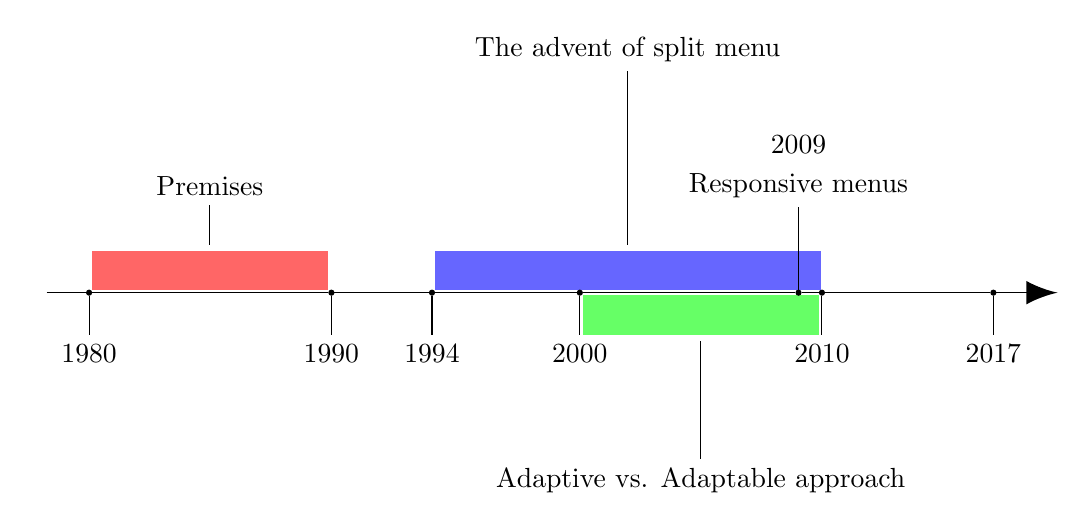
\begin{tikzpicture}[node distance=0.8cm]
	\tikzstyle{circ_xs}
	  =[draw, circle, text width=0.5pt, inner sep=0.5pt]
	\tikzstyle{rect_lg}
	  =[draw, rectangle, text width=3cm, minimum height=.5cm, inner sep=0pt]
	\tikzstyle{rect_xlg}
	  =[draw, rectangle, text width=4.9cm, minimum height=.5cm, inner 
sep=0pt]
	
	\node[draw=none] (start)
	  {};
	  
	\node[circ_xs,draw=black,fill=black] (80)
	  [right=0.5cm of start] {};
	\node[] (1980)
	  [below=0.5cm of 80] {1980};
	  
	\node[rect_lg,fill=red!60,draw=none] (period_premises)
	  [above right=0pt of 80] {};
	\node[outer sep=0pt, inner sep=0pt] (empty1)
	  [above=1pt of period_premises] {};
	\node[] (premises)
	  [above=0.5cm of empty1] {Premises};
	  
	\node[circ_xs,draw=black,fill=black] (90)
	  [right=3cm of 80] {};
	\node[] (1990)
	  [below=0.5cm of 90] {1990};
	  
	\node[circ_xs,draw=black,fill=black] (94)
	  [right=1.2cm of 90] {};
	\node[] (1994)
	  [below=0.5cm of 94] {1994};
	
	\node[rect_xlg,fill=blue!60,draw=none] (period_split)
	  [above right=0pt of 94] {};
	\node[outer sep=0pt, inner sep=0pt] (empty2)
	  [above=1pt of period_split] {};
	\node[] (split_expe)
	  [above=2.2cm of empty2] {The advent of split menu};
	  
	\node[circ_xs,draw=black,fill=black] (00)
	  [right=1.8cm of 94] {};
	\node[] (2000)
	  [below=0.5cm of 00] {2000};
	  
	\node[rect_lg,fill=green!60,draw=none] (period_adapt)
	  [below right=0pt of 00] {};
	\node[outer sep=0pt, inner sep=0pt] (empty3)
	  [below=1pt of period_adapt] {};
	\node[] (adapt)
	  [below=1.5cm of empty3] {Adaptive vs. Adaptable approach};
	
	\node[circ_xs,draw=black,fill=black] (09)
	  [right=2.7cm of 00] {};
	\node[] (2009)
	  [above=1.6cm of 09] {2009};
	\node[] (mobile)
	  [below=0cm of 2009] {Responsive menus};
	
	\node[circ_xs,draw=black,fill=black] (10)
	  [right=0.22cm of 09] {};
	\node[] (2010)
	  [below=0.5cm of 10] {2010};
	
	\node[circ_xs,draw=black,fill=black] (17)
	  [right=2.1cm of 10] {};
	\node[] (2017)
	  [below=0.5cm of 17] {2017};
	  
	\node[circ_xs,draw=white,fill=white] (20)
	  [right=0.4cm of 17] {};
	  
	\node[circ_xs,draw=white,fill=white] (end)
	  [right=0.3cm of 20] {};
	  
	\draw[-] (start)--(80);
	\draw[-] (80)--(90);
	\draw[-] (90)--(94);
	\draw[-] (94)--(00);
	\draw[-] (00)--(09);
	\draw[-] (09)--(10);
	\draw[-] (10)--(17);
	\draw[-] (17)--(20);
	\draw[-latex,line width=0.1cm] (20)--(end);
	
	\draw[-] (80)--(1980);
	\draw[-] (90)--(1990);
	\draw[-] (94)--(1994);
	\draw[-] (00)--(2000);
	\draw[-] (09)--(mobile);
	\draw[-] (10)--(2010);
	\draw[-] (17)--(2017);
	
	\draw[-] (premises)--(empty1);
	\draw[-] (split_expe)--(empty2);
	\draw[-] (adapt)--(empty3);
    \end{tikzpicture}
    \caption{Time line of major research topics from 1980 to 2017.}
  \label{fig:timeline}
\end{figure}

\section{Premises}

Back in the early 80’s, a few researchers conducted a first set of experiments 
to better understand the effects of menu organization on user experience and 
user performance. However the scope of analysis was restrained to static and 
dynamic menu organizations only. Most of these studies resulted to be partially 
useful but they set interesting premises for the next ones.\newline
 
According to \textsc{Sears} and \textsc{Shneiderman} \cite{sears}, 
\textsc{Card} \cite{card} was the first 
researcher to show interest in assessing menu usability. In 1982 already, 
\textsc{Card} 
conducted an experiment based on 3 menu organizations: (1) alphabetically 
ordered items, (2) categorically ordered items and (3) randomly ordered items. 
These menus are depicted by Figure \ref{fig:card_menus}. \textsc{Card} proved 
that 
alphabetically ordered menus were the fastest whereas randomly ordered menus 
were the slowest ones. He also assumed that a \textit{meaningful organization} 
- such as 
alphabetical or categorical ordering - could be beneficial for user 
experience.\newline

\begin{figure}[!ht]
    \centering
    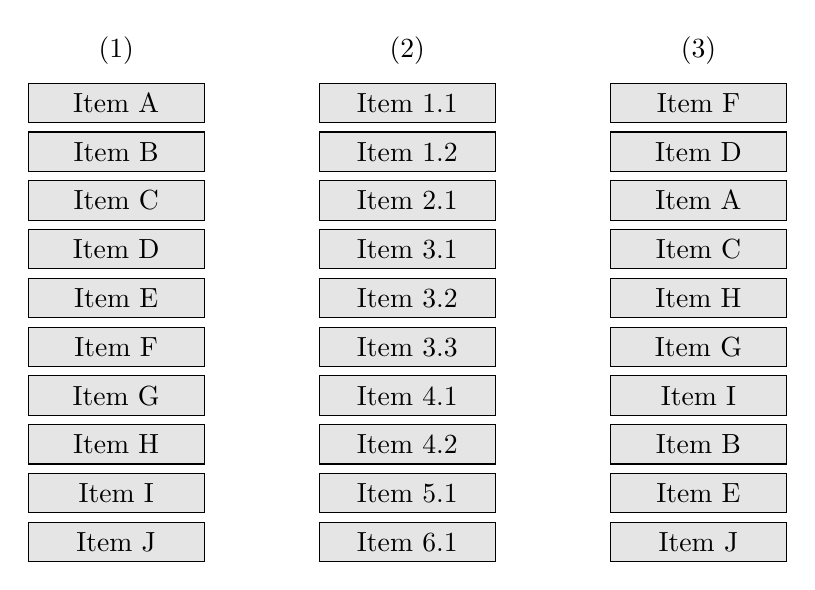
\begin{tikzpicture}[node distance=0.8cm]
        \tikzstyle{item}
	  =[draw, fill=gray!20, rectangle, text width=2cm, 
	  minimum height=0.5cm, text centered]
	
	\node[] (1)
	  {(1)};
	\node[item] (A)
	  [below=3pt of 1]{Item A};
	\node[item] (B)
	  [below=3pt of A] {Item B};
	\node[item] (C)
	  [below=3pt of B] {Item C};
	\node[item] (D)
	  [below=3pt of C] {Item D};
	\node[item] (E)
	  [below=3pt of D] {Item E};
	\node[item] (F)
	  [below=3pt of E] {Item F};
	\node[item] (G)
	  [below=3pt of F] {Item G};
	\node[item] (H)
	  [below=3pt of G] {Item H};
	\node[item] (I)
	  [below=3pt of H] {Item I};
	\node[item] (J)
	  [below=3pt of I] {Item J};
	  
	\node[] (2)
	  [right=3cm of 1] {(2)};
	\node[item] (cat11)
	  [below=3pt of 2] {Item 1.1};
	\node[item] (cat12)
	  [below=3pt of cat11] {Item 1.2};
	\node[item] (cat21)
	  [below=3pt of cat12] {Item 2.1};
	\node[item] (cat31)
	  [below=3pt of cat21] {Item 3.1};
	\node[item] (cat32)
	  [below=3pt of cat31] {Item 3.2};
	\node[item] (cat33)
	  [below=3pt of cat32] {Item 3.3};
	\node[item] (cat41)
	  [below=3pt of cat33] {Item 4.1};
	\node[item] (cat42)
	  [below=3pt of cat41] {Item 4.2};
	\node[item] (cat51)
	  [below=3pt of cat42] {Item 5.1};
	\node[item] (cat61)
	  [below=3pt of cat51] {Item 6.1};
	  
	\node[] (3)
	  [right=3cm of 2]{(3)};
	\node[item] (F2)
	  [below=3pt of 3] {Item F};
	\node[item] (D2)
	  [below=3pt of F2] {Item D};
	\node[item] (A2)
	  [below=3pt of D2] {Item A};
	\node[item] (C2)
	  [below=3pt of A2] {Item C};
	\node[item] (H2)
	  [below=3pt of C2] {Item H};
	\node[item] (G2)
	  [below=3pt of H2] {Item G};
	\node[item] (I2)
	  [below=3pt of G2] {Item I};
	\node[item] (B2)
	  [below=3pt of I2] {Item B};
	\node[item] (E2)
	  [below=3pt of B2] {Item E};
	\node[item] (J2)
	  [below=3pt of E2] {Item J};
    \end{tikzpicture}
    \caption{\textsc{Card}'s menu organizations with 10 items : (1) 
alphabetically, (2) 
categorically and (3) randomly ordered menus.}
    \label{fig:card_menus}
\end{figure}

In 1987, \textsc{Somberg} \cite{somberg} also investigated the effects of menu 
organization on user performance. He replaced \textsc{Card}’s categorically 
ordered menu 
with a new approach based on probability of selection. A probability was bound 
to each item and was modified at each step of the test, displaying different 
menu organizations throughout the entire study. The alphabetical menu was also 
subject to changes as the first displayed letter was chosen randomly from one 
iteration to another. The randomly, alphabetically and probability ordered 
menus were then considered as dynamic menus. These designs are depicted by 
Figure \ref{fig:somberg_menus} which highlights two potential iterations for 
each dynamic menu. The 4th menu organization proposed by the author was called 
\enquote{positionally constant} and consisted of a static alphabetically 
ordered menu. \textsc{Somberg} proved that keeping the items in \textit{fixed 
locations} was more 
performant than allowing the items to move within the menu. Indeed the 
positionally constant menu was prefered and resulted in better user performance 
than dynamic ones.\newline

\begin{figure}[!ht]
    \centering
    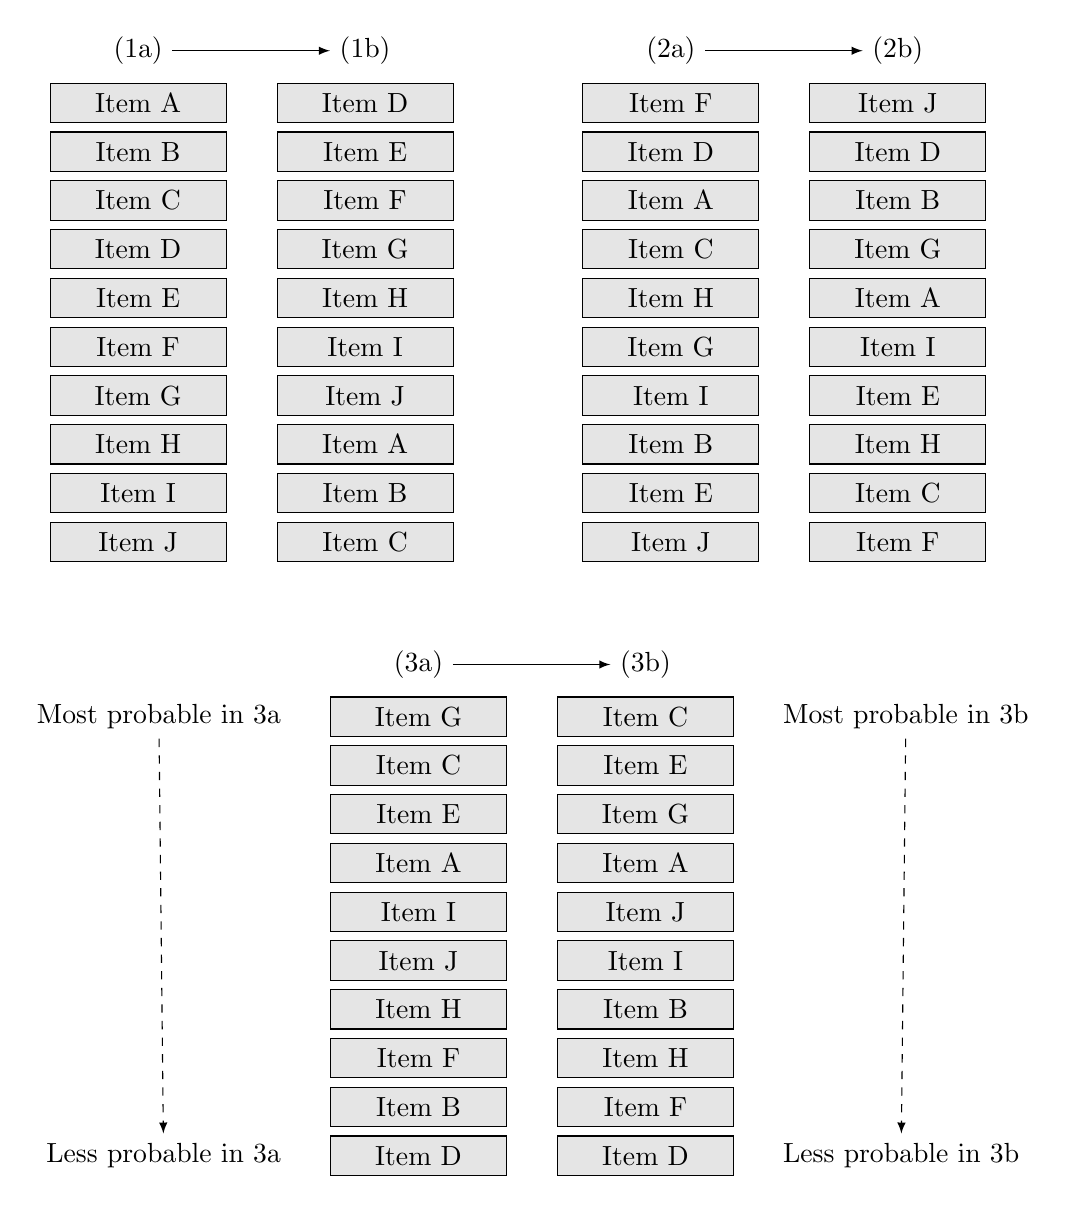
\begin{tikzpicture}[node distance=0.8cm]
        \tikzstyle{item}
	  =[draw, fill=gray!20, rectangle, text width=2cm, 
	  minimum height=0.5cm, text centered]
	
	\node[] (1a)
	  {(1a)};
	\node[item] (A)
	  [below=3pt of 1a]{Item A};
	\node[item] (B)
	  [below=3pt of A] {Item B};
	\node[item] (C)
	  [below=3pt of B] {Item C};
	\node[item] (D)
	  [below=3pt of C] {Item D};
	\node[item] (E)
	  [below=3pt of D] {Item E};
	\node[item] (F)
	  [below=3pt of E] {Item F};
	\node[item] (G)
	  [below=3pt of F] {Item G};
	\node[item] (H)
	  [below=3pt of G] {Item H};
	\node[item] (I)
	  [below=3pt of H] {Item I};
	\node[item] (J)
	  [below=3pt of I] {Item J};
	 
	\node[] (1b)
	  [right=2cm of 1a] {(1b)};
	\node[item] (D3)
	  [below=3pt of 1b] {Item D};
	\node[item] (E3)
	  [below=3pt of D3] {Item E};
	\node[item] (F3)
	  [below=3pt of E3] {Item F};
	\node[item] (G3)
	  [below=3pt of F3] {Item G};
	\node[item] (H3)
	  [below=3pt of G3] {Item H};
	\node[item] (I3)
	  [below=3pt of H3] {Item I};
	\node[item] (J3)
	  [below=3pt of I3] {Item J};
	\node[item] (A3)
	  [below=3pt of J3]{Item A};
	\node[item] (B3)
	  [below=3pt of A3] {Item B};
	\node[item] (C3)
	  [below=3pt of B3] {Item C};

	\node[] (2a)
	  [right=3cm of 1b]{(2a)};
	\node[item] (F2)
	  [below=3pt of 2a] {Item F};
	\node[item] (D2)
	  [below=3pt of F2] {Item D};
	\node[item] (A2)
	  [below=3pt of D2] {Item A};
	\node[item] (C2)
	  [below=3pt of A2] {Item C};
	\node[item] (H2)
	  [below=3pt of C2] {Item H};
	\node[item] (G2)
	  [below=3pt of H2] {Item G};
	\node[item] (I2)
	  [below=3pt of G2] {Item I};
	\node[item] (B2)
	  [below=3pt of I2] {Item B};
	\node[item] (E2)
	  [below=3pt of B2] {Item E};
	\node[item] (J2)
	  [below=3pt of E2] {Item J};
	  
	\node[] (2b)
	  [right=2cm of 2a]{(2b)};
	\node[item] (F4)
	  [below=3pt of 2b] {Item J};
	\node[item] (D4)
	  [below=3pt of F4] {Item D};
	\node[item] (A4)
	  [below=3pt of D4] {Item B};
	\node[item] (C4)
	  [below=3pt of A4] {Item G};
	\node[item] (H4)
	  [below=3pt of C4] {Item A};
	\node[item] (G4)
	  [below=3pt of H4] {Item I};
	\node[item] (I4)
	  [below=3pt of G4] {Item E};
	\node[item] (B4)
	  [below=3pt of I4] {Item H};
	\node[item] (E4)
	  [below=3pt of B4] {Item C};
	\node[item] (J4)
	  [below=3pt of E4] {Item F};
	 
	\node[] (3a)
	  [below right=1cm and 2cm of J] {(3a)};
	\node[item] (F5)
	  [below=3pt of 3a] {Item G};
	\node[item] (D5)
	  [below=3pt of F5] {Item C};
	\node[item] (A5)
	  [below=3pt of D5] {Item E};
	\node[item] (C5)
	  [below=3pt of A5] {Item A};
	\node[item] (H5)
	  [below=3pt of C5] {Item I};
	\node[item] (G5)
	  [below=3pt of H5] {Item J};
	\node[item] (I5)
	  [below=3pt of G5] {Item H};
	\node[item] (B5)
	  [below=3pt of I5] {Item F};
	\node[item] (E5)
	  [below=3pt of B5] {Item B};
	\node[item] (J5)
	  [below=3pt of E5] {Item D};
	  
	\node[] (MostProb3a)
	  [left=0.5cm of F5] {Most probable in 3a};
	\node[] (LessProb3a)
	  [left=0.5cm of J5] {Less probable in 3a};
	  
	\node[] (3b)
	  [right=2cm of 3a]{(3b)};
	\node[item] (F6)
	  [below=3pt of 3b] {Item C};
	\node[item] (D6)
	  [below=3pt of F6] {Item E};
	\node[item] (A6)
	  [below=3pt of D6] {Item G};
	\node[item] (C6)
	  [below=3pt of A6] {Item A};
	\node[item] (H6)
	  [below=3pt of C6] {Item J};
	\node[item] (G6)
	  [below=3pt of H6] {Item I};
	\node[item] (I6)
	  [below=3pt of G6] {Item B};
	\node[item] (B6)
	  [below=3pt of I6] {Item H};
	\node[item] (E6)
	  [below=3pt of B6] {Item F};
	\node[item] (J6)
	  [below=3pt of E6] {Item D}; 
	
	\node[] (MostProb3b)
	  [right=0.5cm of F6] {Most probable in 3b};
	\node[] (LessProb3b)
	  [right=0.5cm of J6] {Less probable in 3b};
	
	\draw[-latex] (1a)--(1b);
	\draw[-latex] (2a)--(2b);
	\draw[-latex] (3a)--(3b);
	\draw[-latex,dashed] (MostProb3a)--(LessProb3a);
	\draw[-latex,dashed] (MostProb3b)--(LessProb3b);
    \end{tikzpicture}
    \caption{Illustrating 2 potential iterations (a) and (b) for each 
\textsc{Somberg}'s dynamic menu organization with 10 items : (1) 
alphabetically, (2) 
randomly and (3) probability ordered menus. (1a) can be considered as the 
static alphabetically ordered menu described by Somberg.}
    \label{fig:somberg_menus}
\end{figure}

In 1985, \textsc{Greenberg} and \textsc{Witten} \cite{greenberg_witten} 
investigated the benefits 
of organizing a menu based on a-priori set of frequencies and updating these 
frequencies according to user’s selections. \textsc{Mitchell} and 
\textsc{Shneiderman} 
\cite{mitchell_shneiderman} provided the first convincing results about such a 
frequency reordering in 1989. They conducted an experiment in which they 
compared a static menu to an automatically reorganized menu based on frequency. 
At first exposure, users preferred, were faster and made fewer errors with the 
static menu. After practice, \textsc{Mitchell} and \textsc{Shneiderman} proved 
that user 
performance was not a problem anymore with the dynamic menu. However this menu 
organization was still not preferred over the static one. They ended up by 
concluding that automatically updating menu organization to reflect the current 
usage patterns might be useful but could also lead to several problems.

\section{The Advent of Split Menu}

In 1994, \textsc{Sears} and \textsc{Shneiderman} \cite{sears} proposed the 
changing concept of 
\textit{split menu}. Based on the early work of \textsc{Greenberg} and 
\textsc{Witten}, \textsc{Smith} and 
\textsc{Mosier} \cite{smith_mosier} were already suggesting in 1986 
\enquote{where some 
data items are used more frequently than others, consider grouping those items 
at the top of the display}. Their solution was articulated in 3 steps: (1) 
maintaining the standard selection mechanism, (2) eliminating the need for 
users to remember additional commands and (3) reorganizing menu items based on 
usage frequency such that the most frequently selected items are moved to the 
top of the menu. 
The founding notions of split menu were finally set.\newline

\textsc{Sears} and \textsc{Shneiderman} defined a split menu as a menu created 
by splitting a menu 
into two sections such as frequently selected items are placed in the top 
section and infrequently selected items are placed in the bottom section. Such 
a 
menu organization proves useful \textit{if and only if} a small subset of the 
menu items represent the majority of selections. This menu organization is 
illustrated by Figure \ref{fig:sears_split} with a dark gray top section above 
the usual alphabetically ordered menu. Notice that most frequently 
selected items are moved to the top section and do not appear anymore in the 
remaining alphabetically ordered menu. Both authors defined a set of 
preliminary guidelines based on initial observations about user's selections 
and refined them into a cognitive model. These guidelines are still applicable 
nowadays and will be explained later in the report considering their 
importance. 
The cognitive model allowed both researchers to prove that (1) a linear model 
could be applied to the infrequently selected items and (2) a logarithmic model 
called \textit{Fitts’ Law} could be applied to the most frequently selected 
items. The linear model illustrates the fact that users spend most of their 
time 
searching an unfamiliar item in a linear fashion by scrolling down the 
given menu. The logarithmic approach proves that users do not scan the entire 
menu when searching for a familiar item but use the order of the menu instead. 
For example, a subject will start at the middle of the menu and will then 
decide 
if the desired item should be above or below this position.\newline

\begin{figure}[!ht]
    \centering
    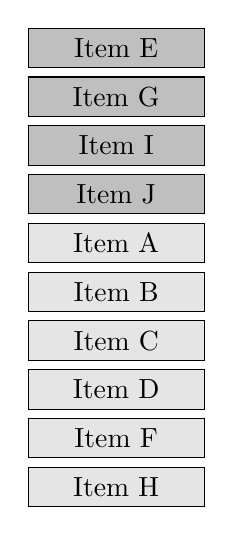
\begin{tikzpicture}[node distance=0.8cm]
        \tikzstyle{item}
	  =[draw, fill=gray!20, rectangle, text width=2cm, 
	  minimum height=0.5cm, text centered]
	
	\node[item,fill=gray!50] (A)
	  {Item E};
	\node[item,fill=gray!50] (B)
	  [below=3pt of A] {Item G};
	\node[item,fill=gray!50] (C)
	  [below=3pt of B] {Item I};
	\node[item,fill=gray!50] (D)
	  [below=3pt of C] {Item J};
	\node[item] (E)
	  [below=3pt of D] {Item A};
	\node[item] (F)
	  [below=3pt of E] {Item B};
	\node[item] (G)
	  [below=3pt of F] {Item C};
	\node[item] (H)
	  [below=3pt of G] {Item D};
	\node[item] (J)
	  [below=3pt of H] {Item F};
	\node[item] (H1)
	  [below=3pt of J] {Item H};
    \end{tikzpicture}
    \caption{\textsc{Sears}' split menu organization with 10 items. The 4 most 
frequently selected items are moved to the top section and displayed in 
alphabetical order.}
    \label{fig:sears_split}
\end{figure}

Split menu provided the missing concept to conciliate both user performance and 
user preference. Indeed \textsc{Sears} and \textsc{Shneiderman} conducted two 
in situ usability 
studies and managed to prove interesting properties: (1) split menu allows to 
enhance user performance only after a short period of one week adjustment, (2) 
split menu allows 17-58\% time savings, (3) 9 out of 13 users expressed 
preference for split menu, (4) 3 out of 13 users expressed no preference and 
(4) 
split menu provides benefits of both frequency ordered and alphabetically 
ordered menus. In conclusion, \textsc{Sears} and \textsc{Shneiderman} proved 
that frequency 
reordering was not sufficient alone. Indeed a \textit{usable} split menu has to 
be 
combined with a traditionally ordered menu and must display the most 
frequently selected items as a \textit{hot list} at the top of this 
traditional menu.\newline

Split menu was widely adopted and implemented in many user interfaces. The most 
renowned split menu is the font menu displayed in Microsoft Word which 
was already used by \textsc{Sears} and \textsc{Shneiderman} to conduct their in 
situ usability studies. However we must wait the early 2000’s to find 
interesting studies about their concrete contextualized efficiency. Paula 
\textsc{Selvidge} \cite{paula} conducted an intensive test to assess split menu 
performance. It was based on 112 tasks to be performed by 73 individuals. She 
proved that split menu was achieving a faster completion time than static menu 
but she also pointed out that they both had the same error rate. Finally she 
identified a clear preference for split menu among participants. James R. 
\textsc{Warren} and Patrick \textsc{Bolton} \cite{warren_bolton} proved that 
split menu was more effective than static menu in the context of ophthalmologic 
diagnoses. They conducted a test with several doctors and found out that a small 
list of 20 diagnoses was mostly used. In this context, a split menu was indeed 
more efficient than a static menu. Mona \textsc{Tom} et al. \cite{mona} proved 
that split menu was also very efficient for automotive mobile multimedia 
applications. Mahamad \textsc{Saipunidzam} et al. \cite{saipu} embedded a split 
menu into a web browser address bar for data entry purposes. They proved that 
(1) it was easier to access Internet and find the desired address through split 
menu and (2) 80\% of participants agreed with the implementation of such a 
split menu in their web browser. In conclusion, many studies confirmed the 
importance and usefulness of split menu to improve both user experience and 
user performance.

\section{Adaptive vs. Adaptable approach}

During the 2000’s, two antagonist notions - respectively called 
\textit{adaptive} and \textit{adaptable} menus - were also prone to discussions 
and researches. Some findings are unclear and highly nuanced but they are still 
worth investigating.\newline

Khalid \textsc{Al-Omar} and Dimitrios \textsc{Rigas} \cite{alomar1} defined the 
concept of \textit{adaptive menu} as \enquote{a system-controlled menu that 
dynamically changes the interface layout and content to each user’s needs}. 
These menus tend to use \textit{graphical} or \textit{spatial techniques} to 
reduce visual search time. A \textit{spatial technique} consists of 
recognizing the most interesting items and copying/moving them for easier 
access. Split menus are based on this notion such that the 
most frequently selected items are moved to the top of the menu. A 
\textit{graphical technique} consists of recognizing the most interesting items 
and then modifying their graphical representation. For example, the most 
frequently selected items could be boldfaced to become catchy for the eyes. 
Both authors defined the concept of \textit{adaptable menu} as \enquote{a 
user-controlled menu that provides techniques which permit the users to adjust 
their layout and content to suit their needs}. Some adaptable menus are said to 
be \textit{coarse-grained} and allow users to move interesting items up or down 
the menu. Others are said to be \textit{fine-grained} and allow users to move 
directly these interesting items to a specific position in the menu. Khalid 
\textsc{Al-Omar} and Dimitrios \textsc{Rigas} finally insisted on a third notion 
called 
\textit{mixed-initiative} which has the ability to combine both adaptable and 
adaptive approaches at the same time. For example, by providing a menu that 
either displays the most frequent or the most recent items in the top section 
and such that this criteria is chosen by the user itself. This type of menu 
can be considered as adaptable and adaptive at the same time because it is 
customized by the system according to the user’s choice. Adaptable, 
adaptive and mixed-initiative menu organizations are depicted by Figure 
\ref{fig:adapt_organizations}.\newline

\begin{figure}[!ht]
    \centering
    \begin{tikzpicture}[node distance=0.8cm]
        \tikzstyle{item}
	  =[draw, fill=gray!20, rectangle, text width=2cm, 
	  minimum height=0.5cm, text centered]
	\tikzstyle{button}
	=[draw, square, text width=0.5cm, minimum height=0.6cm, text centered]
	\tikzstyle{radio_button}
	=[draw, square, text width=0.2cm, minimum height=0.4cm, text centered]
	
	\node[item] (A2)
	  {Item H};
	\node[item] (B2)
	  [below=3pt of A2] {Item A};
	\node[item] (C2)
	  [below=3pt of B2] {Item B};
	\node[item] (D2)
	  [below=3pt of C2] {Item C};
	\node[item] (E2)
	  [below=3pt of D2] {Item D};
	\node[item] (F2)
	  [below=3pt of E2] {Item E};
	\node[item] (G2)
	  [below=3pt of F2] {Item F};
	\node[item] (H2)
	  [below=3pt of G2] {Item G};
	\node[item] (J2)
	  [below=3pt of H2] {Item I};
	\node[item] (H2)
	  [below=3pt of J2] {Item J};
	\node (1)
	  [above=2.3cm of A2] {(1)};
	\node (user)
	  [above=1.8cm of A2] {User-controlled};
	\node (empty)
	  [above=18pt of A2] {};
	\node[button] (up)
	  [above left=3pt and -0.8cm of A2]{$\wedge$};
	\node[button] (down)
	  [above right=3pt and -0.8cm of A2]{$\vee$};
	
	\draw[-latex] (user)--(empty);
	
	\node[item,fill=gray!60] (A)
	  [right=2cm of A2]{Item E};
	\node[item,fill=gray!60] (B)
	  [below=3pt of A] {Item G};
	\node[item,fill=gray!60] (C)
	  [below=3pt of B] {Item I};
	\node[item,fill=gray!60] (D)
	  [below=3pt of C] {Item J};
	\node[item] (E)
	  [below=3pt of D] {Item A};
	\node[item] (F)
	  [below=3pt of E] {Item B};
	\node[item] (G)
	  [below=3pt of F] {Item C};
	\node[item] (H)
	  [below=3pt of G] {Item D};
	\node[item] (J)
	  [below=3pt of H] {Item F};
	\node[item] (H1)
	  [below=3pt of J] {Item H};
	\node (2)
	  [above=2.3cm of A] {(2)};
	\node (syst)
	  [above=1.8cm of A] {System-controlled};
	\node (empty)
	  [above=1pt of A] {};
	  
	\draw[-latex] (syst)--(empty);
	
	\node[item,fill=gray!60] (A3)
	  [right=2cm of A] {Item E};
	\node[item,fill=gray!60] (B3)
	  [below=3pt of A3] {Item G};
	\node[item,fill=gray!60] (C3)
	  [below=3pt of B3] {Item I};
	\node[item,fill=gray!60] (D3)
	  [below=3pt of C3] {Item J};
	\node[item] (E3)
	  [below=3pt of D3] {Item A};
	\node[item] (F3)
	  [below=3pt of E3] {Item B};
	\node[item] (G3)
	  [below=3pt of F3] {Item C};
	\node[item] (H3)
	  [below=3pt of G3] {Item D};
	\node[item] (J3)
	  [below=3pt of H3] {Item F};
	\node[item] (H3)
	  [below=3pt of J3] {Item H};
	\node (3)
	  [above=2.3cm of A3] {(3)};
	\node (user3)
	  [above=1.8cm of A3] {User-controlled};
	\node (empty3)
	  [above=25pt of A3] {};
	\node (empty4)
	  [right=1pt of A3] {};
	\node (syst3)
	  [below right=2pt and -4pt of user3] {System-controlled};
	\node[radio_button] (rec)
	  [above left=3pt and -0.5cm of A3] {};
	\node[radio_button] (freq)
	  [above=3pt of rec] {x};
	\node (freq_text)
	  [right=3pt of freq]{Frequency};
	\node (rec_text)
	  [right=3pt of rec]{Recency};
	  
	\draw[-latex] (user3)--(empty3);
	\draw[-latex] (syst3)|-(empty4);
	  
    \end{tikzpicture}
    \caption{(1) Adaptable, (2) adaptive and (3) mixed-initiative menu 
organizations with a focus on system-controlled and user-controlled features.}
    \label{fig:adapt_organizations}
\end{figure}

Many studies were performed before the work of Khalid \textsc{Al-Omar} and 
Dimitrios 
\textsc{Rigas}. A first controlled lab study compared user performance between a 
static, 
an adaptive and an adaptable split menu. The 
findings were the following: (1) 55\% of the 27 subjects preferred the 
adaptable menu over the adaptive and static ones, (2) the static and adaptable 
split menus were equally performant but allowed a faster selection time than 
the 
adaptive one. A second study involved the traditional Microsoft Word font menu, 
and an adaptable and an adaptive versions of this menu. The experiment proved 
that (1) 65\% of the subjects preferred the adaptable menu, (2) 20\% preferred 
the default font menu and (3) 15\% preferred the adaptive menu. However it is 
important to put these conclusions into perspective because (1) both adaptable 
and adaptive interfaces were very different from the traditional font menu and 
(2) all participants used the adaptable interface before the adaptive approach 
such that they were already used to their own customization choices. A third 
study proved that (1) the adaptable approach was the most performant one, (2) 
adaptive and static split menu were equally performant, (3) 55\% of subjects 
preferred the adaptable approach \textit{if and only if} they received guidance 
to use it efficiently, (4) 30\% of subjects preferred the adaptive alternative 
and (5) 15\% preferred the traditional split menu. In conclusion, the adaptable 
approach seems to be the most preferred and the most performant alternative. 
However the results vary a lot from one study to another in terms of adaptive 
and static menus. Guidance also seems to be an interesting prerequisite to 
enhance user performance and user experience.\newline

Another set of studies restrained their focus on adaptive and static split 
menus. The first study required to perform a set of telephone directory 
searches. The authors proved that the adaptive menu reduced the selection time 
by 35\% and the error rate by 40\% in comparison to the static menu. Moreover 
the adaptive menu was preferred by 69\% of the participants. A second study 
presented different results. Indeed the traditional static approach was 
providing better time performance than the new adaptive one for the first group 
of tasks. It’s only during the second part of the experiment that both menus 
were considered equally performant. In this case it is interesting to point out 
that users preferred the static approach to the adaptive one. In conclusion, it 
seems that the adaptive approach still needs a few tweaks in order to prove a 
concrete usefulness. Notice that both a period of adjustment and guidance 
seem essential for users to become performant with new types of menu 
organization.\newline

In 2005, Teophanis \textsc{Tsandilas} \cite{tsandilas} managed to explain why 
the 
adaptive approach was often disliked by users. He conducted an experiment based 
on 2 different adaptation techniques respectively called \textit{highlighting 
suggestions} and \textit{shrinking non-suggested items}. The first technique 
consisted of highlighting 4 to 8 suggested items based on the user’s cursor 
position. The second one consisted of highlighting 4 to 8 suggested items while 
shrinking the undesired items with a fisheye lens method. Both menu 
organizations are depicted by figure \ref{fig:tsandilas_menus} which 
highlights items A, B, F and H as suggested items. Teophanis \textsc{Tsandilas} 
proved 
that the effectiveness of adaptive techniques may vary along with the accuracy 
of their prediction mechanism. Indeed a low prediction accuracy lead the users 
to untrust the system. And of course user performance vary a lot according to 
this level of accuracy. In conclusion, Teophanis \textsc{Tsandilas} explained 
that 
adaptive mechanisms had to be carefully implemented and tested to 
prove efficient enough.\newline

\begin{figure}[!ht]
    \centering
    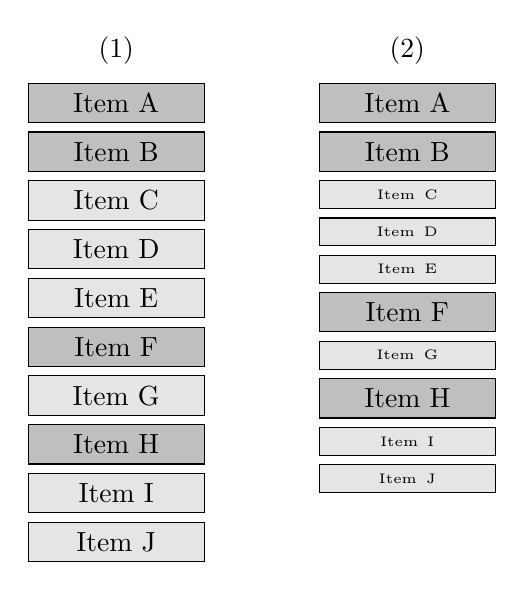
\begin{tikzpicture}[node distance=0.8cm]
        \tikzstyle{item}
	  =[draw, fill=gray!20, rectangle, text width=2cm, 
	  minimum height=0.5cm, text centered]
	\tikzstyle{item-xs}
	  =[draw, fill=gray!20, rectangle, text width=2cm, 
	  minimum height=0.1cm, text centered]
	
	\node[] (1)
	  {(1)};
	\node[item,fill=gray!50] (A)
	  [below=3pt of 1]{Item A};
	\node[item,fill=gray!50] (B)
	  [below=3pt of A] {Item B};
	\node[item] (C)
	  [below=3pt of B] {Item C};
	\node[item] (D)
	  [below=3pt of C] {Item D};
	\node[item] (E)
	  [below=3pt of D] {Item E};
	\node[item,fill=gray!50] (F)
	  [below=3pt of E] {Item F};
	\node[item] (G)
	  [below=3pt of F] {Item G};
	\node[item,fill=gray!50] (H)
	  [below=3pt of G] {Item H};
	\node[item] (I)
	  [below=3pt of H] {Item I};
	\node[item] (J)
	  [below=3pt of I] {Item J};
	  
	\node[] (2)
	  [right=3cm of 1] {(2)};
	\node[item,fill=gray!50] (A2)
	  [below=3pt of 2] {Item A};
	\node[item,fill=gray!50] (B2)
	  [below=3pt of A2] {Item B};
	\node[item-xs] (C2)
	  [below=3pt of B2] {\tiny Item C};
	\node[item-xs] (D2)
	  [below=3pt of C2] {\tiny Item D};
	\node[item-xs] (E2)
	  [below=3pt of D2] {\tiny Item E};
	\node[item,fill=gray!50] (F2)
	  [below=3pt of E2] {Item F};
	\node[item-xs] (G2)
	  [below=3pt of F2] {\tiny Item G};
	\node[item,fill=gray!50] (H2)
	  [below=3pt of G2] {Item H};
	\node[item-xs] (I2)
	  [below=3pt of H2] {\tiny Item I};
	\node[item-xs] (J2)
	  [below=3pt of I2] {\tiny Item J};
    \end{tikzpicture}
    \caption{\textsc{Tsandilas}' menu organizations with 10 items and 
considering that 
items A, B, F and H are the suggested items : (1) highlighting suggestions and 
(2) shrinking non-suggested items.}
    \label{fig:tsandilas_menus}
\end{figure}

In 2010, Khalid \textsc{Al-Omar} and Dimitrios \textsc{Rigas} went even 
further. They conducted 
an experiment based on 5 distinct menu organizations: (1) adaptable menu, (2) 
adaptive split menu, (3) adaptive/adaptable highlighted menu, (3) 
adaptive/adaptable minimised menu and (4) mixed-initiative menu. These new menu 
organizations are depicted by Figure \ref{fig:khalid_menus}. It is interesting 
to notice that the adaptive split menu was divided into 2 top sections. They 
were respectively dedicated to frequency and recency ordering. Each 
organization was respectively tested with a large menu of 29 items and with a 
small menu of 17 items. Both authors found out that user satisfaction was 
affected by the size of the menu. In overall the adaptive/adaptable minimised 
menu was the most preferred approach for the small menu, followed by the 
adaptable and adaptive/adaptable highlighted menus. The worst alternatives were 
the mixed-initiative approach and the adaptive split menu. However the 
mixed-initiative approach was by far the most preferred one for the large menu, 
followed by the adaptive/adaptable minimised interface. Adaptive split menu, 
adaptable and adaptive/adaptable highlighted menus were mostly disliked by the 
participants for the large menu. Therefore Khalid \textsc{Al-Omar} and 
Dimitrios \textsc{Rigas} 
concluded that the \textit{size of personalised content} was a matter of 
concern for 
user satisfaction: (1) users preferred to have less control and receive more 
help from the system for large menus, (2) users preferred when desired items 
were moved to the top section and undesired ones were hidden from the menu and 
(3) the concept of split menu was less efficient for small menus. In other 
words, users prefer adaptable interfaces for small menus because they are more 
likely to customize a small menu than a large one. Indeed a large content 
requires more effort to be understood and used efficiently. Users also liked 
the 
idea of minimising the menu and reducing the number of displayed items. Finally 
both authors made an interesting observation: the recency criteria was not 
used 
by the test participants. Using such a criteria implies to update the menu each 
time a selection is performed. Therefore the menu is constantly being modified 
and it becomes confusing for users.\newline

\begin{figure}[!ht]
    \centering
    \begin{tikzpicture}[node distance=0.8cm]
        \tikzstyle{item}
	  =[draw, fill=gray!20, rectangle, text width=2cm, 
	  minimum height=0.5cm, text centered]
	\tikzstyle{button}
	=[draw, square, text width=0.5cm, minimum height=0.6cm, text centered]
	\tikzstyle{radio_button}
	=[draw, square, text width=0.2cm, minimum height=0.4cm, text centered]
	
	\node[item] (A)
	  {Item B};
	\node[item] (B)
	  [below=3pt of A] {Item A};
	\node[item] (C)
	  [below=3pt of B] {Item C};
	\node[item] (D)
	  [below=3pt of C] {Item D};
	\node[item] (E)
	  [below=3pt of D] {Item J};
	\node[item] (F)
	  [below=3pt of E] {Item F};
	\node[item] (G)
	  [below=3pt of F] {Item G};
	\node[item] (H)
	  [below=3pt of G] {Item H};
	\node[item] (I)
	  [below=3pt of H] {Item I};
	\node[item] (J)
	  [below=3pt of I] {Item E};
	\node[button] (up)
	  [above left=3pt and -0.8cm of A]{$\wedge$};
	\node[button] (down)
	  [above right=3pt and -0.8cm of A]{$\vee$};  
	\node[] (1)
	  [above=1.2cm of A]{(1)};
	
	\node[item,fill=gray!60] (A2)
	  [right=0.5cm of A]{Item B};
	\node[item,fill=gray!60] (B2)
	  [below=3pt of A2] {Item F};
	\node[item,fill=gray!85] (C2)
	  [below=3pt of B2] {Item A};
	\node[item,fill=gray!85] (D2)
	  [below=3pt of C2] {Item H};
	\node[item] (E2)
	  [below=3pt of D2] {Item C};
	\node[item] (F2)
	  [below=3pt of E2] {Item D};
	\node[item] (G2)
	  [below=3pt of F2] {Item E};
	\node[item] (H2)
	  [below=3pt of G2] {Item G};
	\node[item] (I2)
	  [below=3pt of H2] {Item I};
	\node[item] (J2)
	  [below=3pt of I2] {Item J};
	\node[] (2)
	  [above=1.2cm of A2]{(2)};
	
	\node[item,fill=gray!60] (A3)
	  [right=0.5cm of A2]{Item B};
	\node[item] (B3)
	  [below=3pt of A3] {Item A};
	\node[item] (C3)
	  [below=3pt of B3] {Item C};
	\node[item,fill=gray!60] (D3)
	  [below=3pt of C3] {Item D};
	\node[item] (E3)
	  [below=3pt of D3] {Item J};
	\node[item,fill=gray!60] (F3)
	  [below=3pt of E3] {Item F};
	\node[item,fill=gray!60] (G3)
	  [below=3pt of F3] {Item G};
	\node[item] (H3)
	  [below=3pt of G3] {Item H};
	\node[item] (I3)
	  [below=3pt of H3] {Item I};
	\node[item] (J3)
	  [below=3pt of I3] {Item E};
	\node[button] (up)
	  [above left=3pt and -0.8cm of A3]{$\wedge$};
	\node[button] (down)
	  [above right=3pt and -0.8cm of A3]{$\vee$};  
	\node[] (3)
	  [above=1.2cm of A3]{(3)};
	  
	\node[item] (A4)
	  [right=0.5cm of A3]{Item B};
	\node[item] (B4)
	  [below=3pt of A4] {Item D};
	\node[item] (C4)
	  [below=3pt of B4] {Item F};
	\node[item] (D4)
	  [below=3pt of C4] {Item G};
	\node[item] (E4)
	  [below=3pt of D4] {Item A};
	\node[item] (F4)
	  [below=3pt of E4] {Item C};
	\node[button] (down4)
	  [below=3pt of F4] {$\vee$};
	\node[] (4)
	  [above=1.2cm of A4]{(4)};
	  
	\node[item,fill=gray!60] (A5)
	  [right=0.5cm of A4]{Item B};
	\node[item,fill=gray!60] (B5)
	  [below=3pt of A5] {Item D};
	\node[item,fill=gray!60] (C5)
	  [below=3pt of B5] {Item F};
	\node[item,fill=gray!60] (D5)
	  [below=3pt of C5] {Item G};
	\node[item] (E5)
	  [below=3pt of D5] {Item A};
	\node[item] (F5)
	  [below=3pt of E5] {Item C};
	\node[item] (G5)
	  [below=3pt of F5] {Item E};
	\node[item] (H5)
	  [below=3pt of G5] {Item H};
	\node[item] (I5)
	  [below=3pt of H5] {Item I};
	\node[item] (J5)
	  [below=3pt of I5] {Item J};
	\node[] (5)
	  [above=1.2cm of A5]{(5)};
	\node[radio_button] (rec)
	  [above left=3pt and -0.5cm of A5] {};
	\node[radio_button] (freq)
	  [above=3pt of rec] {x};
	\node (freq_text)
	  [right=3pt of freq]{Frequency};
	\node (rec_text)
	  [right=3pt of rec]{Recency};
    \end{tikzpicture}
    \caption{\textsc{Al-Omar} and \textsc{Rigas}' menu organizations with 10 
items : (1) 
adaptable, (2) adaptive split, (3) adaptive/adaptable highlighted, (4) 
adaptive/adaptable minimised and (5) mixed-initiative menus.}
    \label{fig:khalid_menus}
\end{figure}

\section{Responsive menus}
In 2009, Yusuke \textsc{Fukazawa} et al. \cite{fukazawa} focused their 
researches on 
menus for mobile phones, observing an increasing complexity in mobile 
interfaces. They conducted an experiment that last 6 days with 20 participants. 
Each subject was given an additional Windows mobile phone configured with 3 
distinct menu organizations described as \textit{responsive}. A 
\textit{responsive menu} 
is designed with the idea that mobile screens are smaller than desktop 
computers and that menus should therefore be adapted to this constraint. 
\textsc{Fukazawa} et al. developed 3 responsive menu organizations (see 
Figure \ref{fig:fukazawa_menus}). The 
first one was made of 2-column items and was displaying the most important 
items 
at the top. The last two menus were displaying varying item sizes: the more 
important the item was, the bigger it was displayed. Yusuke \textsc{Fukazawa} et 
al. 
observed that 70\% of the participants were both satisfied by the new menu 
organizations and by the prediction function used to identify important items. 
However they noticed that \textit{master users} were showing higher preferences 
for old menus and \textit{novice users} were more satisfied by new menu 
organizations.\newline

\begin{figure}[!ht]
    \centering
    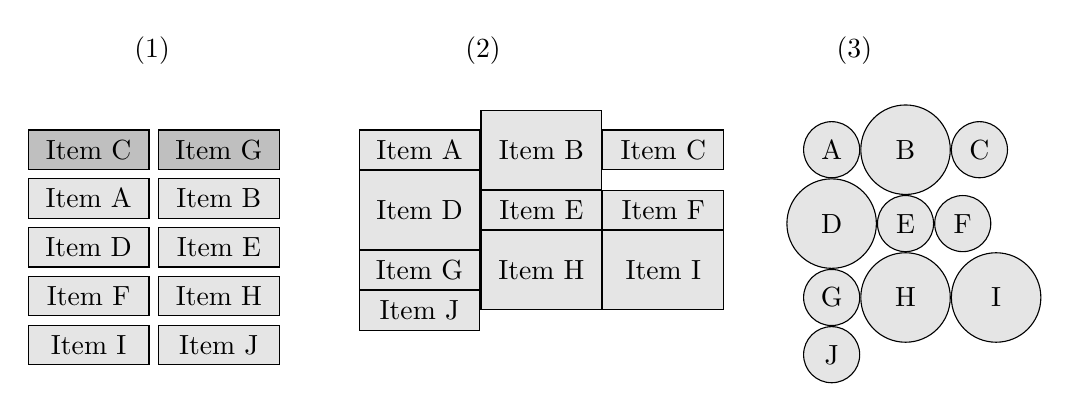
\begin{tikzpicture}[node distance=0.8cm]
	\tikzstyle{item}
	  =[draw, fill=gray!20, rectangle, text width=2cm, 
	  minimum height=0.5cm, text centered]
	  
        \tikzstyle{item_col}
	  =[draw, fill=gray!20, rectangle, text width=1.3cm, 
	  minimum height=0.5cm, text centered]
	\tikzstyle{item_col_xl}
	  =[draw, fill=gray!20, rectangle, text width=1.3cm, 
	  minimum height=1cm, text centered]
	  
	\tikzstyle{item_circle}
	  =[draw, fill=gray!20, circle, text width=0.3cm, text centered]
	\tikzstyle{item_circle_xl}
	  =[draw, fill=gray!20, circle, text width=0.8cm, text centered]
	  
	\node[item_col, fill=gray!50] (A)
	  {Item C};
	\node[item_col] (B)
	  [below=3pt of A] {Item A};
	\node[item_col] (C)
	  [below=3pt of B] {Item D};
	\node[item_col] (D)
	  [below=3pt of C] {Item F};
	\node[item_col] (E)
	  [below=3pt of D] {Item I};
	\node[item_col, fill=gray!50] (F)
	  [right=3pt of A] {Item G};
	\node[item_col] (G)
	  [below=3pt of F] {Item B};
	\node[item_col] (H)
	  [below=3pt of G] {Item E};
	\node[item_col] (I)
	  [below=3pt of H] {Item H};
	\node[item_col] (J)
	  [below=3pt of I] {Item J};
	\node[] (1)
	  [above right=0.7cm and -9pt of A]{(1)};
	  
	\node[item_col] (A2)
	  [right=1cm of F]{Item A};
	\node[item_col_xl] (B2)
	  [right=0pt of A2] {Item B};
	\node[item_col] (C2)
	  [right=0pt of B2] {Item C};
	\node[item_col_xl] (D2)
	  [below=0pt of A2] {Item D};
	\node[item_col] (E2)
	  [right=0pt of D2] {Item E};
	\node[item_col] (F2)
	  [right=0pt of E2] {Item F};
	\node[item_col] (G2)
	  [below=0pt of D2] {Item G};
	\node[item_col_xl] (H2)
	  [right=0pt of G2] {Item H};
	\node[item_col_xl] (I2)
	  [right=0pt of H2] {Item I};
	\node[item_col] (J2)
	  [below=0pt of G2] {Item J};
	\node[] (2)
	  [above right=0.7cm and -9pt of A2]{(2)};
	  
	\node[item_circle] (A3)
	  [right=1cm of C2]{A};
	\node[item_circle_xl] (B3)
	  [right=0pt of A3] { B};
	\node[item_circle] (C3)
	  [right=0pt of B3] { C};
	\node[item_circle_xl] (D3)
	  [below=0pt of A3] { D};
	\node[item_circle] (E3)
	  [right=0pt of D3] { E};
	\node[item_circle] (F3)
	  [right=0pt of E3] { F};
	\node[item_circle] (G3)
	  [below=0pt of D3] { G};
	\node[item_circle_xl] (H3)
	  [right=0pt of G3] { H};
	\node[item_circle_xl] (I3)
	  [right=0pt of H3] { I};
	\node[item_circle] (J3)
	  [below=0pt of G3] { J};
	\node[] (3)
	  [above right=0.7cm and -9pt of A3]{(3)};
	  
	
    \end{tikzpicture}
    \caption{\textsc{Fukazawa}'s menu organizations with 10 items : (1) 
2-column, (2) rectangle-shaped items and (3) circle-shaped items.}
    \label{fig:fukazawa_menus}
\end{figure}

\section{Learning outcomes}
Lots of interesting findings have been highlighted by these previous 
researches. 
First, \textsc{Card} proved that a \textit{meaningful organization} of menu 
items such 
as alphabetical or categorical ordering was beneficial for user experience. 
\textsc{Somberg} later proved that \textit{positionally constant} menus were 
preferred 
by users such that items should not move too much within the menu. He also 
identified that a \textit{period of adjustment} was required to handle 
efficiently new menu organizations. Then \textsc{Sears} and 
\textsc{Shneiderman} managed to find 
the right balance between dynamic and static menus by introducing the concept 
of 
\textit{split menu}. It is a great example that combines almost positionally 
constant menu, frequency-ordering and meaningful organization. Experiments 
conducted before Khalid \textsc{Al-Omar} and Dimitrios \textsc{Rigas} proved 
that 
\textit{adaptable approach} was the most preferred alternative. They also 
proved that both a \textit{period of adjustment} and \textit{guidance} were 
necessary prerequisites for users to understand new menu organizations. 
Teophanis \textsc{Tsandilas} later explained that the \textit{accuracy 
prediction} of 
the adaptive mechanism was critical for the adaptive approach to be performant. 
Finally Khalid \textsc{Al-Omar} and Dimitrios \textsc{Rigas} proved that users 
were showing 
preferences for their \textit{minimised menu} because it was hiding unwanted 
items and therefore displaying less items at the same time. They also proved 
that split menu was less efficient for small menus and highlighted the fact 
that alternatives may be required for small screens. Yusuke \textsc{Fukazawa} et 
al. 
investigated this possibility and implemented \textit{responsive} menus. They 
identified varying reactions between \textit{master} and \textit{novice users}. 
Indeed master users like to have more control and novice users prefer to be 
helped by the system. Master users also showed preferences for traditional menus 
because they were already use to them.

\chapter{Methodology}
The methodology is mainly inspired by the previous researches described in the 
state of the art. A set of 11 hypotheses are described and argued based on the 
learning outcomes of the previous chapter. Then, the experimental method that 
aims to confirm or reverse these hypotheses is deeply reviewed. Finally, the 
related implementation is reported for computer scientists’ interests.

\section{Hypotheses} \label{hypotheses}
A set of 11 hypotheses have been initially formulated. Each hypothesis is based 
on one or several learning outcomes from one or several researchers. The 
objective is to study the field of research even further than the previous 
experiments. The hypotheses will be later confirmed or reversed by the 
experiment. Some new hypotheses may even be formulated afterwards with respect 
to the results of the experiment.

\begin{itemize}
 \item \textbf{H1a:} the split menu reduces the selection time.
 \item \textbf{H1b:} the split menu is preferred 
by users.
\end{itemize}

\textsc{Sears} and \textsc{Shneiderman} proved that a split menu following a 
strict set of 
guidelines could be beneficial for both user experience and user performance. 
Therefore, a menu providing a hot list of items based on frequency reordering 
should indeed reduce selection time and receive a higher user 
preference.

\begin{itemize}
  \item \textbf{H2a:} the minimised menu reduces the selection time.
  \item \textbf{H2b:} the minimised menu is preferred by users.
\end{itemize}

Khalid \textsc{Al-Omar} and Dimitrios \textsc{Rigas} identified a clear user 
preference for their minimised menu. Such a menu hides unwanted items and 
therefore reduces the number of items displayed on the screen. This is very 
related to the \textit{rules of ergonomy} taught by Professor Jean Vanderdonckt 
in his course entitled \enquote{human-computer interaction} at Univeristé 
Catholique de Louvain (BE). One HCI rule called \enquote{rule of thumb} states 
that an interface should display a minimum of 4 items and a maximum of 8. 
Unfortunately, this rule is still neglected by the researchers. The idea is to 
implement a menu which displays a restricted number of items at the same time. 
It should be easier to read and manipulate for users, especially for novice 
ones.

\begin{itemize}
  \item \textbf{H3a:} the responsive menu reduces the selection time.
  \item \textbf{H3b:} the responsive menu is preferred by users.
\end{itemize}

Yusuke \textsc{Fukazawa} studied the effects of menu organization with a 
specific focus towards small mobile screens. He proved that a responsive menu 
organization could be beneficial for user experience. Unfortunately, his work 
must still be argued by further experiments. Since this master thesis aims to 
conceive and design a menu organization for smartphone, it is necessary to 
include his findings in the experimental method. Therefore, a responsive menu 
should be designed and tested.

\begin{itemize}
  \item \textbf{H4a:} novice users show a preference for the adaptive menus.
  \item \textbf{H4b:} master users show a preference for the traditional menu.
\end{itemize}

Yusuke \textsc{Fukazawa} found out that \textit{master users} preferred to have 
more 
control over menu customization and preferred to be less guided by the system. 
Therefore, they showed higher preferences for traditional and adaptable menus 
because they are respectively use to it and user-controlled. Our experiment is 
mainly focused towards adaptive menus and master users should therefore show a 
preference for traditional menu organizations only. At the opposite, 
\textit{novice users} showed higher preferences for adaptive menus which prove 
the system ability to handle menu customization by itself. They should show the 
same preferences during our experiment.

\begin{itemize}
  \item \textbf{H5a:} guidance informations help users to understand how a 
menu 
works.
  \item \textbf{H5b:} guidance informations help users to handle a menu more 
efficiently.
  \item \textbf{H5c:} a period of adjustment helps users to handle a menu more 
efficiently.
\end{itemize}

Khalid \textsc{Al-Omar} and Dimitrios \textsc{Rigas} proved that users needed 
both \textit{guidance informations} and a \textit{period of adjustment} in 
order to handle and understand new menu organizations, especially for adaptable 
menus. The experiment should however provide the same results for adaptive menus 
since they still represent new menu organizations for users. Notice that 
\textsc{Somberg}, and \textsc{Sears} and \textsc{Shneiderman} also observed 
that a period of adjustment was beneficial for user performance during their 
respective experiments.

\section{Experimental method}
The experimental method aims to confirm or reverse the hypotheses. In 
order to achieve this objective, 8 menu organizations have been designed and 
implemented in an Android application developed especially for the 
experiment. This subsection argues the choices performed during the development 
of the experimental method. It also describes its overall operation.

\subsection{Test protocol} \label{test_protocol}
Participants were first asked to answer a preliminary set of sociodemograhic 
questions on a survey paper. In order to prevent users from being distracted 
by a second computer screen, it was decided to use a paper version of the 
survey. It is available at the end of the dissertation, see Appendix 
\ref{survey}. The users were then asked to perform 2 kinds of sessions on the 
Android application. The first sessions were called 
\textit{training sessions} - or \textit{adjustment periods} in reference to 
\textsc{Somberg}' study \cite{somberg}. Each training session last for 2 
consecutive selections and was preceded by guidance informations. For each 
selection, the system randomly chose an item and displayed it on the screen. 
Once the menu was displayed, the participant had to press on the 
required item. Guidance informations were used to help users to understand the 
following menu organization. A second set of sessions was organized after the 8 
training sessions. These new sessions were called \textit{evaluation sessions} 
and last for 10 consecutive selections. An evaluation session was not preceded 
by guidance informations but was followed by a set of questions to answer on 
the survey paper. These questions were used to assess the usability of the menu 
organization and gather user's feedback. During the evaluation sessions, 6 
parameters were recorded for each selection: (1) the the required item, (2) 
its 
position in the menu, (3) the selected item, (4) its position in the menu, (5) 
the selection time and (6) the correctness of the selection.

\subsection{Items}
The items displayed by the Android application have been selected from a 
controlled experiment conducted by \textsc{Findlater} \cite{findlater}. This 
experiment 
used 16 items divided into 4 specific categories. Notice that Khalid 
\textsc{Al-Omar} and 
Dimitrios \textsc{Rigas} considered such a menu as a \textit{small} one during 
their own 
study \cite{alomar1}. Figure \ref{fig:items} depicts the categories of items 
described by \textsc{Findlater} and used during the experiment.\newline

\begin{figure}[!ht]
    \centering
    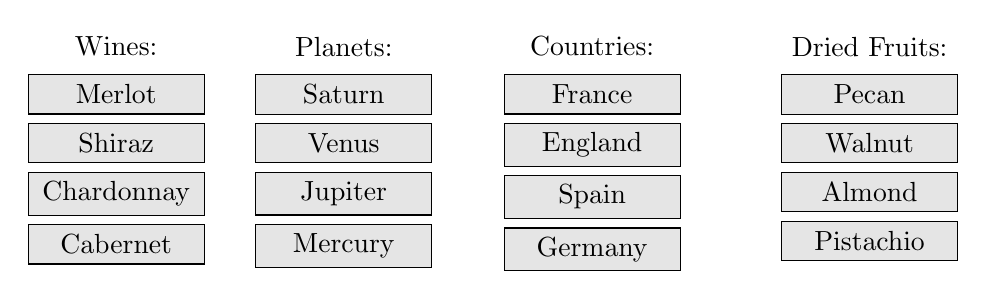
\begin{tikzpicture}[node distance=0.8cm]
        \tikzstyle{item}
	  =[draw, fill=gray!20, rectangle, text width=2cm, 
	  minimum height=0.5cm, text centered]
	
	\node[] (wines)
	  {Wines:};
	\node[item] (A)
	  [below=3pt of wines]{Merlot};
	\node[item] (B)
	  [below=3pt of A] {Shiraz};
	\node[item] (C)
	  [below=3pt of B] {Chardonnay};
	\node[item] (D)
	  [below=3pt of C] {Cabernet};
	  
	\node[] (planets)
	  [right=1.5cm of wines] {Planets:};
	\node[item] (cat11)
	  [below=3pt of planets] {Saturn};
	\node[item] (cat12)
	  [below=3pt of cat11] {Venus};
	\node[item] (cat21)
	  [below=3pt of cat12] {Jupiter};
	\node[item] (cat31)
	  [below=3pt of cat21] {Mercury};
	 
	\node[] (countries)
	  [right=1.5cm of planets]{Countries:};
	\node[item] (F2)
	  [below=3pt of countries] {France};
	\node[item] (D2)
	  [below=3pt of F2] {England};
	\node[item] (A2)
	  [below=3pt of D2] {Spain};
	\node[item] (C2)
	  [below=3pt of A2] {Germany};
	  
	\node[] (dried)
	  [right=1.5cm of countries]{Dried Fruits:};
	\node[item] (F3)
	  [below=3pt of dried] {Pecan};
	\node[item] (D3)
	  [below=3pt of F3] {Walnut};
	\node[item] (A3)
	  [below=3pt of D3] {Almond};
	\node[item] (C3)
	  [below=3pt of A3] {Pistachio};
    \end{tikzpicture}
    \caption{The 4 categories of 4 items described by \textsc{Findlater} and 
used 
during the experiment.}
    \label{fig:items}
\end{figure}

\subsection{Control condition menu}
A control condition menu stands as baseline to perform the comparison between a 
set of menu organizations. For this experiment, a traditional vertical menu 
was chosen to be the control condition menu. It consisted of a 1-column menu 
which displayed the items in categorical order such that wines were grouped 
together, followed by planets, countries and dried fruits in the order 
displayed 
by Figure \ref{fig:items}.
%The control 
%condition menu organization is depicted by Figure \ref{fig:control_menu}.

% \begin{figure}[!ht]
%     \centering
    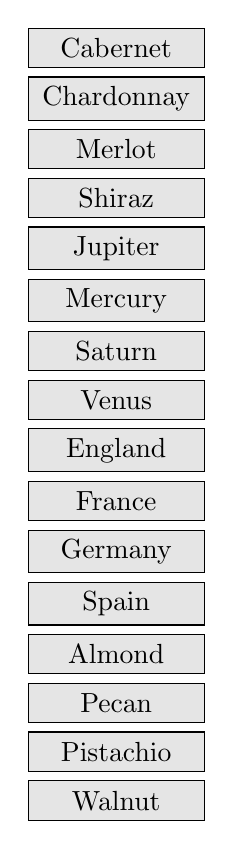
\begin{tikzpicture}[node distance=0.8cm]
        \tikzstyle{item}
	  =[draw, fill=gray!20, rectangle, text width=2cm, 
	  minimum height=0.5cm, text centered]

	\node[item] (A)
	  {Cabernet};
	\node[item] (B)
	  [below=3pt of A] {Chardonnay};
	\node[item] (C)
	  [below=3pt of B] {Merlot};
	\node[item] (D)
	  [below=3pt of C] {Shiraz};
	\node[item] (E)
	  [below=3pt of D] {Jupiter};
	\node[item] (F)
	  [below=3pt of E] {Mercury};
	\node[item] (G)
	  [below=3pt of F] {Saturn};
	\node[item] (H)
	  [below=3pt of G] {Venus};
	\node[item] (I)
	  [below=3pt of H] {England};
	\node[item] (J)
	  [below=3pt of I] {France};
	\node[item] (K)
	  [below=3pt of J] {Germany};
	\node[item] (L)
	  [below=3pt of K] {Spain};
	\node[item] (M)
	  [below=3pt of L] {Almond};
	\node[item] (N)
	  [below=3pt of M] {Pecan};
	\node[item] (O)
	  [below=3pt of N] {Pistachio};
	\node[item] (P)
	  [below=3pt of O] {Walnut};
    \end{tikzpicture}
    \caption{Control condition menu organization with the 16 items described by 
Findlater.}
%     \label{fig:control_menu}
% \end{figure}

\subsection{Split menu}
We followed the guidelines described by \textsc{Sears} and \textsc{Shneiderman} 
in order to 
confirm the hypotheses related to the split menu. Indeed, both authors defined 
a 
strict set of guidelines to design efficient split menus. As explained 
previously, these guidelines are based on 3 preliminary observations: (1) 
users know the name of the item they are looking for, (2) some items are 
more frequently selected than others and (3) these most frequent items are 
ideally not already located at the top of the menu. These preliminary 
observations are met during the experiment because users have to select items 
that are chosen and displayed by the system. \textsc{Sears} and 
\textsc{Shneiderman} developed 3 
guidelines based on these observations: (1) both the hot list and the 
traditional sections should respect the traditional ordering, (2) the hot list 
should not display more than 4 items and (3) the hot list should only display 
the most frequently selected items.\newline

For the experiment purpose, the hot list was decided to hold 3 items as 
\textsc{Findlater} used during his own study \cite{findlater}. The hot list was 
also 
decided to be highlighted. Therefore, the background of the hot list items was 
displayed in a dark blue colour called \textit{primary colour} in the initial 
Android theme.

\subsection{Minimised menu}
Traditional menus display the entire set of items at the same time. The users 
usually require to scroll down the menu to show the last items. Minimised menu 
aims to reduce the number of displayed items. Following the \textit{rule of 
thumb} described in the section \ref{hypotheses}, we designed a menu divided 
into consecutive and distinct \textit{pages}. Each page displays at most 8 
items. Since our initial set of items is made of 16 items, each menu 
organization is divided into 2 pages of exactly 8 items.

\subsection{Responsive menu}
The main objective of a responsive menu is to adapt the menu organization to 
the small size of mobile screens. The idea is to reduce both the size of 
displayed items and the margins in between these items. Sometimes it also 
consists of 
reducing the number of displayed items but we already implemented this 
opportunity with minimised menus. The responsive menu implemented for the 
experiment is designed with 2 columns of items. The first item is displayed in 
the top left column, the second one is displayed in the top right column and so 
on for the next items.

\subsection{Mixed-initiative menus}
Khalid \textsc{Al-Omar} and Dimitrios \textsc{Rigas} defined a 
\textit{mixed-initiative} menu as 
a menu that combines both adaptive and adaptable properties. During the 
experiment, a mixed-initiative menu was a menu organization combining split, 
minimised and/or responsive properties. Therefore 2x2x2 menu organizations have 
been designed to implement all the potential combinations of 
menus. These configurations are described in the following section and 
screenshots from the Android application are provided to better visualize the 
different menu organizations, see Appendix \ref{screenshots}.

\section{Implementation}
An Android application called \textit{Menuz} has been implemented to conduct 
the experiment. The application was responsible for displaying the menus and 
providing their guidance informations. It has also been designed to act as a 
guide during the experiment and therefore to give relevant directives to the 
participants. This subsection describes the architecture and choices performed 
during its implementation. Screenshots of the application are provided by 
Appendix \ref{screenshots}.

\subsection{Application architecture}
The Android application has been developed with \textit{Android Studio}. It is 
divided into 13 activities, 13 related XML layouts and Java classes, and one 
additional Java class for utility purpose. An android activity takes care of 
creating a window. It is first described by a XML layout in which Android 
components are assembled to form its UI. An additional Java class must also be 
implemented for each activity. This class allows to manage the activity 
lifecycle but also to react to user’s actions through listeners. Figure 
\ref{fig:activity} illustrates the concept of activity through the combination 
of an XML layout and a Java class.\newline

\begin{figure}[!ht]
    \centering
    \begin{tikzpicture}[node distance=0.8cm]
        \tikzstyle{file}
	  =[draw, rectangle, text width=2cm, minimum height=3cm, 
	  text centered]
	\tikzstyle{rect_xs}
	  =[draw, rectangle, text width=1.1cm, minimum height=.13cm, 
	  text centered]
	\tikzstyle{rect_xxs}
	  =[draw, rectangle, text width=0.7cm, minimum height=.1cm, 
	  text centered]
	  
	\node[file] (filexml) {};
	\node[] (xml) 
	  [above=3pt of filexml] {activity\_main.xml};
	\node[] (code1) 
	  [below left=9pt and -2.4cm of xml] {\_\_\_\_\_};
	\node[] (code2) 
	  [below left=3pt and -1.45cm of code1] {\_\_\_\_};
	\node[] (code3) 
	  [below left=3pt and -1.7cm of code2] {\_\_\_\_\_};
	\node[] (code4) 
	  [below left=3pt and -1.15cm of code3] {\_\_\_};
	\node[] (code5) 
	  [below left=3pt and -1.4cm of code4] {\_\_\_\_};
	  
	\node[file] (filejava)
	  [right=3cm of filexml] {};
	\node[] (java) 
	  [above=3pt of filejava] {MainActivity.java};
	\node[] (code6) 
	  [below left=9pt and -2.4cm of java] {\_\_\_\_\_};
	\node[] (code7) 
	  [below left=3pt and -1.45cm of code6] {\_\_\_\_};
	\node[] (code8) 
	  [below left=3pt and -1.7cm of code7] {\_\_\_\_\_};
	\node[] (code9) 
	  [below left=3pt and -1.15cm of code8] {\_\_\_};
	\node[] (code10) 
	  [below left=3pt and -1.4cm of code9] {\_\_\_\_};
	
	\node[inner sep=0, outer sep=0, draw=black, fill=black, 
	line width=0.06cm] (empty) 
	  [right=1.5cm of filexml] {};
	\node[] (empty1)
	  [below=1pt of empty] {};
	  
	\node[file] (windowfile)
	  [below=2.5cm of empty] {};
	\node[] (window) 
	  [above=3pt of windowfile] {window};
	\node[] (title)
	  [below=2.9cm of empty] {\_\_\_\_};
	\node[rect_xs] (textinput)
	  [below=3.8cm of empty] {};
	\node[rect_xxs] (button)
	  [below=4pt of textinput] {\_\_};
	
	\draw[-latex, line width=0.1cm] (empty)--(filexml);
	\draw[-latex, line width=0.1cm] (empty)--(filejava);
	\draw[-latex, dashed, line width=0.05cm] (empty1)--(window);
    \end{tikzpicture}
    \caption{An activity takes care of creating a window by combining a XML 
layout which defines its UI and a Java class which handles the activity 
lifecycle and user's actions.}
    \label{fig:activity}
\end{figure}

The entire application architecture is depicted by Figure 
\ref{fig:architecture}. The first activity is called \textit{MainActivity}. It 
welcomes the user and requires him to enter a username before starting the 
experiment. This first window is followed by an activity called 
\textit{IntroductionActivity} which introduces the course of the experiment. 
The 
user then receives the guidance informations of the first menu. Guidance 
informations are provided by an activity called 
\textit{MenuIntroductionActivity}. Its purpose is to introduce 
the new menu organizations to the subjects of the experiment. It leads to a 
fourth activity called \textit{NextSelectionActivity} which chooses a random 
item to be picked by the users. It also contains a selection counter to show 
the progress of the experiment. A selection timer starts when the participant 
presses on the \enquote{ready} button and once the menu has been entirely 
displayed on the screen. Each menu is designed to be a distinct activity. The 
activity is 
stopped when the user has performed a selection and the 
\textit{NextSelectionActivity} is called upon to display the next required item. 
The process is repeated until the 8 training sessions and the 8 evaluation 
sessions have been successfully achieved. Notice that a fifth activity called 
\textit{SurveyRequestActivity} is started at the end of each evaluation session 
to recall the user that he must answer a set of questions on the survey paper. 
During these evaluation sessions, \textit{MenuIntroductionActivity} doesn't 
display guidance informations anymore but acts as an intermediary window to 
announce the start of the next evaluation session. Finally, a class called 
\textit{Utility} has been implemented to allow developers to set up the 
experiment from one single file.\newline

\begin{figure}[!ht]
    \centering
    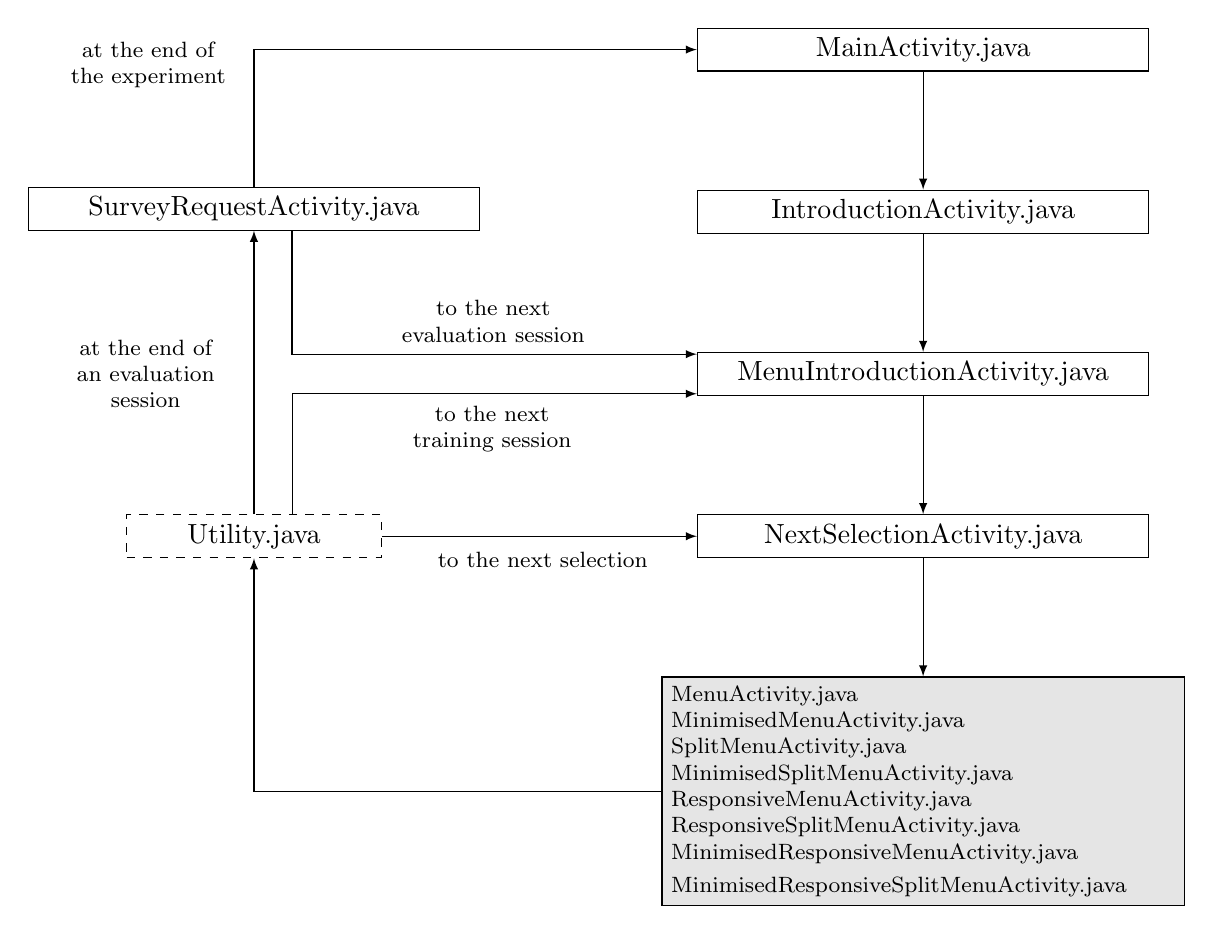
\begin{tikzpicture}[node distance=0.8cm]
        \tikzstyle{item}
	  =[draw, rectangle, text width=5.5cm, 
	  minimum height=0.5cm, text centered]
	\tikzstyle{item_xs}
	  =[draw, rectangle, text width=3cm, 
	  minimum height=0.5cm, text centered]
	\tikzstyle{item_xl}
	  =[draw, rectangle, text width=6.4cm, 
	  minimum height=0.5cm]
	
	\node[item] (main)
	  {MainActivity.java};
	\node[item] (intro)
	  [below= 1.5cm of main]{IntroductionActivity.java};
	\node[item] (menuintro)
	  [below= 1.5cm of intro]{MenuIntroductionActivity.java};
	\node[item] (nextselection)
	  [below= 1.5cm of menuintro]{NextSelectionActivity.java};
	\node[item_xl, fill=gray!20] (menu)
	  [below= 1.5cm of nextselection] 
	  {\footnotesize{MenuActivity.java\\ 
	  MinimisedMenuActivity.java\\
	  SplitMenuActivity.java\\
	  MinimisedSplitMenuActivity.java\\
	  ResponsiveMenuActivity.java\\
	  ResponsiveSplitMenuActivity.java\\
	  MinimisedResponsiveMenuActivity.java\\
	  MinimisedResponsiveSplitMenuActivity.java}};
	 
	\node[item_xs, dashed] (utility)
	  [left= 4cm of nextselection] {Utility.java};
	\node[item] (survey)
	  [above= 3.6cm of utility] {SurveyRequestActivity.java};
	 
	\node[] (end_evalb)
	  [left=6cm of menuintro] {\footnotesize{an evaluation}};
	\node[] (end_evala)
	  [above=-3pt of end_evalb] {\footnotesize{at the end of}};
	\node[] (end_evalc)
	  [below=-3pt of end_evalb] {\footnotesize{session}};
	  
	\node[] (to_nextb)
	  [above left=0cm and 1.3cm of menuintro] 
	  {\footnotesize{evaluation session}};
	\node[] (to_nexta)
	  [above=-3pt of to_nextb] {\footnotesize{to the next}};
	  
	\node[] (to_nextd)
	  [below left=0cm and 1.75cm of menuintro] 
	  {\footnotesize{to the next}};
	\node[] (to_nexte)
	  [below=-3pt of to_nextd] {\footnotesize{training session}};
	  
	\node[] (to_nextc)
	  [below left=-0.2cm and 0.5cm of nextselection] 
	  {\footnotesize{to the next selection}};
	
	\node[] (end)
	  [left= 6cm of main] {\footnotesize{at the end of}};
	\node[] (end b)  
	  [below=-3pt of end]{\footnotesize{the experiment}};
	
	\draw[-latex] (main)--(intro);
	\draw[-latex] (intro)--(menuintro);
	\draw[-latex] (menuintro)--(nextselection);
	\draw[-latex] (nextselection)--(menu);
	
	\draw[-latex] (menu)-|(utility);
	\draw[-latex] (utility)--(survey);
	\draw[-latex] (utility)--(nextselection);
	\draw[-latex] (utility.30)|-(menuintro.185);
	\draw[-latex] (survey.330)|-(menuintro.175);
	\draw[-latex] (survey)|-(main);
    \end{tikzpicture}
    \caption{Application architecture.}
    \label{fig:architecture}
\end{figure}

\subsection{Activities}
This second subsection describes the overal operation and the content of each 
activity and the additional \textit{Utility} class implemented in the Android 
application.

\subsubsection{MainActivity}
\textit{MainActivity.java} is the first activity called at the start of the 
application. The window is made of a \textit{TextView}, an \textit{EditText} 
and a \textit{Button}. The \textit{TextView} is an interface element that 
displays text to the user \cite{android_textview}. In this case, it is 
used to welcome the user to the application. The \textit{EditText} is 
a UI element for entering and modifying text \cite{android_edittext}. It is 
used 
to enter a username that will be saved when the user presses the button. Notice 
that a \textit{cheatcode} can be used to jump directly to a specific menu 
organization. The cheatcode must start with the \enquote{\#} character and must 
be followed by the id of the menu organization. In this case, the participant 
will be redirected to the \textit{MenuIntroductionActivity} which announces the 
start of the corresponding evaluation session.

\subsubsection{IntroductionActivity}
This second activity is started by \textit{MainActivity}. It is made of 5 
\textit{TextView} widgets and a \textit{Button}. Each \textit{TextView} is used 
as a title or as a paragraph and aims to introduce the course of the 
experiment and its overall operation to the user.

\subsubsection{MenuIntroductionActivity}
\textit{MenuIntroductionActivity} is called at the beginning of each session. 
Before a training session, it provides guidance informations about the next 
menu organization. Before an evaluation session, it is only used as an 
intermediary window to announce to the subject that a new evaluation session 
is about to start. The XML layout is made of 3 \textit{TextView} and 1 
\textit{Button}. The third \textit{TextView} is hidden before an evaluation 
session because there is only one sentence to display.\newline

The activity is also responsible to reset the \textit{parameter arrays} and 
the \textit{selection counter}. A \textit{parameter array} is a Java array used 
to store the values recorded during the experiment. There are 6 interesting 
parameters to monitor for the experiment purpose: (1) the required items, (2) 
the positions of the required items, (3) the selected items, (4) the position 
of the selected items, (5) the selection time for each selected item and (6) 
the correctness of the selection. The 6th parameter is not recorded as an 
array. It is measured later by the \textit{Utility} class. 
\textit{MenuIntroductionActivity} must also reset the \textit{selection counter} 
since it is called before the start of a new session. Finally, it must 
increment the \textit{menu counter}.

\subsubsection{NextSelectionActivity}
\textit{NextSelectionActivity} is an activity called before a selection must 
be performed. It is responsible for choosing the next required item, 
displaying this choice on the screen and starting the appropriate menu 
organization when the user presses the \enquote{ready} button. Items are 
selected by following the approach taken by \textsc{Findlater} \cite{findlater} 
: a ZipF 
distribution (Zpifian $R^2=.99$) over 8 randomly chosen items for each menu 
organization to avoid the learning effect between sessions. Zipf's law is an 
empirical law concerning the frequency of words in a language. It was developed 
by the Americain linguist George Kingsley Zipf and refers to the fact that some 
words are more frequently used than others and such that their selection 
frequencies can be approximated with a Zipfian distribution.\newline

The activity is made of 1 \textit{Button} and 4 \textit{TextView}. The 1st 
\textit{TextView} corresponds to the title, the second one to a directive, the 
3rd one is responsible for displaying the required item and the 4th one
consists of a counter which represents the progress of the experiment.

\subsubsection{Activities related to menu organizations}
As explained previously, 2x2x2 menu organizations were implemented for the 
experiment. Each menu organization represents a control condition menu, a split 
menu, a minimised menu, a responsive menu or a mixed-initiative menu. A 
mixed-initiative menu is the result of the combination between one or several 
types of menu among split, minimised and/or responsive. Each menu organization 
was designed to be a distinct activity. Two initial 
methods are required for these activities. The first one, called 
\textit{onCreate()}, is responsible for providing relevant directives in 
order to create the window. It displays the menu according to the XML layout 
and may eventually apply a few modifications if required. This method is the 
most basic function required by an Android activity. The second method, called 
\textit{selectionPerformed()}, is perfomed when a user chooses an 
item in the menu. It is responsible for calling the \textit{Utility} class 
that will save the relevant parameters and redirect the user to the next 
activity.\newline

\textbf{MenuActivity} represents the control condition menu. It is made of 
one column within which all items are displayed vertically. Users require to 
scroll down the menu to see the last items. It comprises the most basic 
implementation of both methods \textit{onCreate()} and 
\textit{selectionPerformed()}.\newline

\textbf{MinimisedMenuActivity} carries a self-descriptive name. It 
represents the minimised menu organization. It consists of a vertical menu 
divided into 2 pages. Each page is made of 2 categories of 4 items and no 
scrolling is required to see the last items of a page. A page is 
also accessible through \enquote{previous/next} arrows respectively located in 
the bottom left and bottom right corner of the menu organization. The previous 
or next arrows are only displayed if respectively a previous or a next page 
is available. Two additional methods have been implemented to handle these 
buttons. They are respectively called \textit{previousProposals()} and 
\textit{nextProposals()}.\newline

\textbf{SplitMenuActivity} represents a split menu organization. It is very 
similar to \textit{MenuActivity}. Indeed, it corresponds to a 
vertical menu but it displays the 3 most frequent items at the top of it. These 
items are highlighted with a blue colour and highlightings are handled by the 
method \textit{onCreate()}.\newline

\textbf{MinimisedSplitMenuActivity} corresponds to the first 
mixed-initiative menu presented to a participant. It combines both 
minimised and split menu properties. Therefore, it consists of a menu 
divided into 2 pages such that each page displays 8 items and the first 
page displays the 3 most frequently selected items at the top of the menu. 
These items are also highlighted with a blue colour and no scrolling is 
required to see the last items of a page. It is implemented with the 
additional methods \textit{previousProposals()} and 
\textit{nextProposals()}. Highlightings are handled by these methods 
and the method \textit{onCreate()}.\newline

\textbf{ResponsiveMenuActivity} represents a responsive menu 
organization. It consists of a menu divided into 2 columns within 
which the items are displayed opposite to each others. This new menu 
organization allows to display all the items on the screen of the smartphone 
used during the experiment. Therefore, no scrolling is required to see the last 
items.\newline

\textbf{ResponsiveSplitMenuActivity} combines responsive and split menu 
properties. It is very similar to \textit{ResponsiveMenuActivity} but 
it displays the 3 most frequently selected items at the top of the menu. These 
items are highlighted with a blue colour and highlightings are handled by the 
method \textit{onCreate()}.\newline

\textbf{MinimisedResponsiveMenuActivity} is a mixed-initiative menu 
that combines minimised and responsive menu properties. It is divided 
into 2 pages such that each page is itself divided into 2 columns 
within which the items are displayed opposite to each other. Each page is made 
of 2 categories of 4 items and is accessible through \enquote{previous/next} 
arrows. The additional methods \textit{previousProposals()} and 
\textit{nextProposals()} have been implemented to handle these buttons. 
Notice that a navigation arrow is only displayed if necessary.\newline

\textbf{MinimisedResponsiveSplitMenuActivity} represents the 
combination of minimised, responsive and split menu properties. 
Therefore, it is very similar to \textit{MinimisedResponsiveMenuActivity} 
but it displays the 3 most frequently selected items at the top of the menu for 
the first page only. These items are highlighted with a blue colour and the 
highlightings are handled by the methods \textit{onCreate()}, 
\textit{previousProposals()} and \textit{nextProposals()}.

\subsubsection{SurveyRequestActivity}
\textit{SurveyRequestActivity} is an activity called at the end of an 
evaluation session by the \textit{Utility} class. It is used to recall the user 
that he must answer a set of questions on the survey paper, or to announce the 
end of the experiment and thank him for its participation. The UI is made of 3 
\textit{TextView} and 1 \textit{Button}. At the end of all evaluation 
sessions, the button redirects the user to the \textit{MainActivity}. 
Otherwise, it redirects the user to the next \textit{MenuIntroductionActivity}.

\subsubsection{Utility}
As described previously, \textit{Utility} is not an Android activity but a 
traditional Java class instead. It is used to set up the experiment from one 
single file. For example, a developer can modify the length of the sessions, 
update the list of items or even change the way parameters are gathered and 
printed. The class is essential for the application and almost all classes call 
one of its methods at some point of their execution.
\chapter{Results}

During the experiment, some interesting properties were assessed using the 
survey paper while other parameters were recorded by the Android application. 
This chapter aims to collect, classify and analyze these records to 
achieve 3 objectives. First, to confirm or reverse the hypotheses, then 
possibly to formulate new hypotheses and finally to assess the usability of 
new menu organizations. As explained earlier, usability is measured with 3 
interesting properties: (1)  effectiveness, (2) efficiency and (3) 
satisfaction. This section first describes the participants who took part to 
the experiment and then analyzes these usability-related properties one after 
the other. The hypotheses are finally discussed at the end of the chapter.

\section{Participants}

The study was conducted with 18 French speaking subjects between 17 and 61 
years old. To avoid bias due to language, the application and the survey 
used during the experiment were translated in French. Moreover, the experiment 
has been conducted with the same smartphone for each participant. The 
smartphone was a Sony Xperia M2 with a 4.8 inches screen. Half the 
participants were men while the other half was women. Parity gender was 
therefore achieved.\newline

The subjects come from various backgrounds that we have grouped in 4 
distinct categories: (1) engineers, (2) art school students/workers, (3) other 
academics, and (5) others. \textit{Engineers} and \textit{art school 
students/workers} were enough to get their own representative 
category. \textit{Other academics} consisted of 1 law student, 1 foreign 
language student, 1 psychology student and 1 physical education student. 
Finally, 2 administrative employees, 1 worker, 1 saleswoman and 1 pupil were 
part of the last category called \textit{others}. Figure \ref{fig:participants} 
(a) depicts the distribution of participants according to their educational 
background. It also highlights the distribution of men and women among these 
categories. Notice that men are mainly representing engineering and artistic 
careers in our participant sample. Women are mostly representing other academics 
and other careers. Unfortunately, the parity gender is not well represented by 
a distribution based on the educational background.

\begin{figure}[!ht]
    
  \begin{subfigure}[t]{.49\textwidth}
  \centering
  \resizebox{\linewidth}{!}{
  \begin{tikzpicture}[baseline]
    \begin{axis}[
      %title={Evolution of student participation for each exercise},
      enlarge y limits=false,
      axis lines*=left,
      %xlabel={Educational background},
      ylabel={\# participants},
      %xmin=1, xmax=4,
      ymin=1, ymax=6,
      xtick=data,
      ytick={1,2,3,4,5,6},
      legend pos=east,
      legend columns=0,
      %xmajorgrids=true,
      ymajorgrids=true,
      grid style=dashed,
      enlargelimits=0.15,
      %histogram related :
      ybar,
      symbolic x coords={engineers, art school, other academics, others},
      nodes near coords,
      xticklabel style={
	inner sep=0pt,
	anchor=north east,
	rotate=45
      }
      ]
      
    \addplot[blue!50!black, fill=blue!55] coordinates
    {(engineers, 4) (art school, 3) (other academics, 1) (others, 1)};   
    \addplot[red!70!black, fill=red!35] coordinates
    {(engineers, 1) (art school, 1) (other academics, 3) (others, 4)}; 
    
    \legend{Men, Women}
    
    \end{axis}
  \end{tikzpicture}}
  \caption{Distribution of participants according to their educational 
background.}
  \label{fig:background}
  \end{subfigure}
  \begin{subfigure}[t]{.49\textwidth}
    \resizebox{\linewidth}{!}{
    \centering
    \begin{tikzpicture}[baseline]
    \begin{axis}[
      %title={Evolution of student participation for each exercise},
      enlarge y limits=false,
      axis lines*=left,
      xlabel={Age group},
      ylabel={\# participants},
      %xmin=1, xmax=4,
      ymin=1, ymax=6,
      xtick=data,
      ytick={1,2,3,4,5,6},
      legend pos=east,
      legend columns=0,
      %xmajorgrids=true,
      ymajorgrids=true,
      grid style=dashed,
      enlargelimits=0.15,
      %histogram related :
      ybar,
      symbolic x coords={<25, 25-40, >40 years old},
      nodes near coords,
      ]
      
    \addplot[blue!50!black, fill=blue!55] coordinates
    {(<25, 5) (25-40, 2) (>40 years old, 2)};   
    \addplot[red!70!black, fill=red!35] coordinates
    {(<25, 4) (25-40, 2) (>40 years old, 3)};
    
    \legend{Men, Women}
    
    \end{axis}
  \end{tikzpicture}}
  \caption{Distribution of participants according to their age group.}
  \label{fig:age_range}
  \end{subfigure}
  \caption{}
    \label{fig:participants}
\end{figure}

Figure \ref{fig:participants} (b) depicts the distribution 
of participants according to their age group. It also highlights gender 
distribution. Most participants were between 18 and 25 but each age group was 
at 
least represented once during the experiment. We were able to form and use the 
3 
following groups of participants during the analysis: (1) <25, (2) 25-40 and 
(3) >40 years old. Parity gender is very well represented among these 
categories. Therefore it can be appropriate to distinguish gender and age groups 
during the analysis.\newline

Participants were also asked to rate their skills with smartphones and 
touch screen technologies. The objective was to differentiate 2 groups of 
subjects: (1) novice and (2) master users. Unfortunately, smartphone users 
and touch screens are becoming more common nowadays and we haven't found 
enough novice users for the experiment. Even subjects without smartphones 
considered themselves rather efficient with touch screens and smartphones. 
Therefore, we will not be able to prove the hypothesis based on novice 
users and their preference for adaptive menus. Figure 
\ref{fig:participants_skills} illustrates the distribution of participants' 
responses about their skills with smartphones and 
touch screens. Notice that a rating ranging from 1 (bad) to 7 (excellent) was 
at their disposal to assess their abilities.

\begin{figure}[!ht]
      \centering
  \begin{tikzpicture}
    \begin{axis}[
      %title={Evolution of student participation for each exercise},
      width=11cm,
      enlarge y limits=false,
      axis lines*=left,
      xlabel={Rating},
      ylabel={\# participants},
      xmin=1, xmax=7,
      ymin=1, ymax=10,
      xtick=data,
      ytick={0,1,2,3,4,5,6,7,8,9,10},
      legend pos=east,
      legend columns=0,
      %xmajorgrids=true,
      ymajorgrids=true,
      grid style=dashed,
      enlargelimits=0.15,
      %histogram related :
      ybar,
      symbolic x coords={1,2,3,4,5,6,7},
      nodes near coords,
      ]
      
    \addplot[green!40!black, fill=green!65] coordinates
    { (1,0) (2,1) (3,2) (4,2) (5,3) (6,1) (7,9)};   
    \addplot[orange!70!black, fill=orange!30] coordinates
    { (1,0) (2,1) (3,1) (4,0) (5,4) (6,3) (7,9)};
    
    \legend{w/ Smartphone, w/ Touch screen}
    
    \end{axis}
  \end{tikzpicture}
  \caption{Distribution of participants according to their own estimations of 
their skills with smartphones and touch screens.}
  \label{fig:age_range}
    \label{fig:participants_skills}
\end{figure}

\section{Effectiveness}
Effectiveness is the first property to evaluate in order to assess the 
usability of a menu organization. According to the Oxford English Dictionary, 
effectiveness can be defined as \enquote{the degree to which something is 
successful in producing a desired result; success} \cite{effectiveness}. In 
1998, effectiveness was defined more precisely by HCI researchers in 
the ISO9241-11 standard which describes it as \enquote{the accuracy and 
completeness of users' 
tasks while using a system} \cite{iso}. Indeed, when using the 
menu of a computer system, a user wishes to fulfill a precise action - e.g. 
saving a document - and must press the related menu item - e.g. the button 
\enquote{save} - in order 
to execute this action. In other words, the effectiveness of a menu 
organization can be assessed by observing its average error rate. A low error 
rate means that users have managed to produce the desired results by pressing 
the correct buttons during the experiment. The control condition menu 
displayed 
by \textit{MenuActivity} can be used to benchmark the effectiveness between 
menu organizations. A lower error rate than \textit{MenuActivity} means that 
the users have managed to produce the desired results more frequently with new 
menu 
organizations.\newline

Figure \ref{fig:errors} (a) depicts the average error rate for each 
menu organization. The control condition menu (1) and the split menu (3) seem 
to be the worst menu organizations in terms of effectiveness. The new menu 
organizations showed better results as users achieved lower error rates when 
using them. Even more interesting, the users did not commit any mistake when 
using the responsive menu (5). However, notice that the worst 
average error rate does not even exceed $3.33\%$. In conclusion, all 
the displayed menu organizations can be considered as greatly effective.

\begin{figure}[!ht]
    
  \begin{subfigure}[t]{.49\textwidth}
  \centering
  \resizebox{\linewidth}{!}{
  \begin{tikzpicture}[baseline]
    \begin{axis}[
      %title={Evolution of student participation for each exercise},
      enlarge y limits=false,
      axis lines*=left,
      xlabel={Menu organization},
      ylabel={Average error rate (\%)},
      xmin=1, xmax=8,
      ymin=1, ymax=10,
      xtick=data,
      %ytick={0,1,2,4},
      legend pos=east,
      legend columns=0,
      %xmajorgrids=true,
      ymajorgrids=true,
      grid style=dashed,
      enlargelimits=0.15,
      %histogram related :
      ybar,
      symbolic x coords={1,2,3,4,5,6,7,8},
      nodes near coords,
      ]
      
    \addplot[orange!70!black, fill=orange!30] coordinates
    {(1,3.3333) (2,0.5556) (3,3.3333) (4,1.6667) (5,0) (6,1.6667) (7,1.1111) 
     (8,0.5556)};
    
    %\legend{Men, Women}
    
    \end{axis}
  \end{tikzpicture}}
  \caption{Average error rate for each menu organization.}
  \label{fig:background}
  \end{subfigure}
  \begin{subfigure}[t]{.49\textwidth}
    \resizebox{\linewidth}{!}{
    \centering
    \begin{tikzpicture}[baseline]
    \begin{axis}[
      %title={Evolution of student participation for each exercise},
      enlarge y limits=false,
      axis lines*=left,
      xlabel={Age group},
      ylabel={Average error rate (\%)},
      %xmin=1, xmax=4,
      ymin=1, ymax=10,
      xtick=data,
      %ytick={1,2,3,4,5,6},
      legend pos=east,
      legend columns=0,
      %xmajorgrids=true,
      ymajorgrids=true,
      grid style=dashed,
      enlargelimits=0.15,
      %histogram related :
      ybar,
      symbolic x coords={<25, 25-40, >40 years old},
      nodes near coords,
      ]
      
    \addplot[blue!50!black, fill=blue!55] coordinates
    {(<25, 2.8) (25-40, 0) (>40 years old, 1.9)};   
    \addplot[red!70!black, fill=red!35] coordinates
    {(<25, 0) (25-40, 1.3) (>40 years old, 2.5)};
    
    \legend{Men, Women}
    
    \end{axis}
  \end{tikzpicture}}
  \caption{Average error rate according to the age group and the gender 
distinction.}
  \label{fig:age_range}
  \end{subfigure}
  \caption{}
    \label{fig:errors}
\end{figure}

Figure \ref{fig:errors} (b) depicts the average error rate according to 
the age group. It also highlights gender distinction and shows that men are 
slightly less effective than women. In general, they commit more mistakes than 
women. However, women tend to commit more and more errors over the years. Older 
participants show the worst average error rate while the intermediary age group 
shows the best average error rate.

\begin{figure}[!ht]
    \centering
\begin{tikzpicture}
    \begin{axis}[
      %title={Evolution of student participation for each exercise},
      enlarge y limits=false,
      enlarge x limits=-1,
      height=6cm,
      width=14.5cm,
      axis lines*=left,
      xlabel={Participant id},
      ylabel={\# errors},
      xmin=1, xmax=18,
      ymin=0, ymax=6,
      xtick=data,
      ytick={0,1,2,3,4,5,6},
      legend pos=east,
      legend columns=0,
      %xmajorgrids=true,
      ymajorgrids=true,
      grid style=dashed,
      enlargelimits=0.15,
      %histogram related :
      ybar,
      symbolic x coords={1,2,3,4,5,6,7,8,9,10,11,12,13,14,15,16,17,18},
      nodes near coords,
      ]
      
    \addplot[orange!70!black, fill=orange!40] coordinates
    {(1,1) (2,0) (3,2) (4,0) (5,0) (6,2) (7,1) (8,5) (9,1) (10,4) (11,1) (12,0)
     (13,0) (14,2) (15,0) (16,2) (17,1) (18,0)};
    
    %\legend{Men, Women}
    
    \end{axis}
  \end{tikzpicture}
  \caption{Number of errors performed by each participant after 80 
selections.}
    \label{fig:errors_participants}
\end{figure}

It is finally interesting to observe more precisely the errors performed during 
the experiment. Figure \ref{fig:errors_participants} 
illustrates the distribution of errors among the subjects of the 
experiment. We can first notice that nearly half the mistakes were 
performed by 2 participants. These subjects made 4 and 5 errors 
which is respectively 4 and 5 times greater than the average number of 
mistakes performed by each participant. A deeper analysis of mistakes 
allowed us to identify 4 types of errors: (1) forgetting, (2) touch screen 
imprecision, (3) inattention and (4) confusion. Some participants complained 
about \textit{forgetting} the required item because it disappeared once the menu 
was displayed. The problem occured 9 times as illustrated by Figure 
\ref{fig:errors_types}. It corresponds to nearly half the mistakes performed 
during the study. The \textit{imprecision} mistake also occured a few times. It 
happened when subjects ended up pressing on a button instead of scrolling down 
the menu, or when they ended up pressing on a button above or below the 
desired item. The \textit{inattention} error occured when 
the hot list of a split menu was updated and users were not attentive enough to 
these changes. Therefore, they ended up pressing on a wrong button. Finally, 
\textit{confusion} happened a few times between the words \enquote{Germany} and 
\enquote{England}, and \enquote{Walnut} and \enquote{Pecan} due to the fact that 
these words are pretty close to each other in french (Allemagne/Angleterre and 
Noix/Noix de Pecan).

\begin{figure}[!ht]
    \centering
\begin{tikzpicture}
    \begin{axis}[
      %title={Evolution of student participation for each exercise},
      enlarge y limits=false,
      enlarge x limits=-1,
      height=6cm,
      width=14.5cm,
      axis lines*=left,
      xlabel={Type of mistake},
      ylabel={\# errors},
      %xmin=1, xmax=4,
      ymin=0, ymax=10,
      xtick=data,
      ytick={0,2,4,6,8,10},
      legend pos=east,
      legend columns=0,
      %xmajorgrids=true,
      ymajorgrids=true,
      grid style=dashed,
      enlargelimits=0.15,
      %histogram related :
      ybar,
      symbolic x coords={forgetting, imprecision, inattention, confusion},
      nodes near coords,
      ]
      
    \addplot[orange!70!black, fill=orange!30] coordinates
    {(forgetting,9) (imprecision,6) (inattention,4) (confusion,3)};
    
    %\legend{Men, Women}
    
    \end{axis}
  \end{tikzpicture}
  \caption{Distribution of errors among the 4 identified types of mistakes.}
    \label{fig:errors_types}
\end{figure}

\section{Efficiency}
Effiency is the second interesting property to observe when assessing menu 
usability. According to the Oxford English Dictionary, efficiency is defined as 
\enquote{the ratio of the useful work performed by a machine or in a process to 
the total energy expended or heat taken in} \cite{efficiency}. In 1998, HCI 
researchers defined the term more rigourously with the ISO9241-11 standard. 
They described it as \enquote{the resources expended by the user in relation to 
the 
accuracy and completeness of goals achieved} \cite{iso}. In other 
words, a computer system is said to be efficient if users manage to reach 
their goals while expending as little resources as possible. Therefore, we 
should 
focus on observing lower selection time for new menu organizations compared to 
the 
control condition menu. It is also relevant to adopt a \textit{productivity} 
approach such that we can observe the ratio of successful selection rate 
(useful output) to average required selection time (input). Figure 
\ref{fig:selectime} (a) depicts the average selection time for 
each menu organization. It shows that all menu organizations reduce the 
selection time in comparison to the control condition menu (1), except for the 
minimised menu (2) which slightly increases this value. The responsive 
menu (5) is once again the most performant one. Figure 
\ref{fig:selectime} (b) illustrates the productivity ratio for each menu 
organization. All menu organizations can be considered as more efficient than 
the traditional menu. The productivity approach also confirms that the 
responsive menu is the most performant one. Indeed, it provides the best 
results 
in terms of effectiveness (lower error rate) and efficiency (lower selection 
time).

\begin{figure}[!ht]
    
  \begin{subfigure}[t]{.49\textwidth}
  \centering
  \resizebox{\linewidth}{!}{
  \begin{tikzpicture}[baseline]
    \begin{axis}[
      %title={Evolution of student participation for each exercise},
      enlarge y limits=false,
      axis lines*=left,
      xlabel={Menu organization},
      ylabel={Average selection time (s)},
      xmin=1, xmax=8,
      ymin=2, ymax=3,
      xtick=data,
      ytick={2,2.2,2.4,2.6,2.8,3},
      legend pos=east,
      legend columns=0,
      %xmajorgrids=true,
      ymajorgrids=true,
      grid style=dashed,
      enlargelimits=0.15,
      %histogram related :
      ybar,
      symbolic x coords={1,2,3,4,5,6,7,8},
      nodes near coords,
      ]
      
    \addplot[orange!70!black, fill=orange!30] coordinates
    {(1,2.497) (2,2.517) (3,2.464) (4,2.260) (5,2.067) (6,2.314) (7,2.351) 
     (8,2.322)};
    
    %\legend{Men, Women}
    
    \end{axis}
  \end{tikzpicture}}
  \caption{Average selection time for each menu organization.}
  \label{fig:background}
  \end{subfigure}
  \begin{subfigure}[t]{.49\textwidth}
    \resizebox{\linewidth}{!}{
    \centering
    \begin{tikzpicture}[baseline]
    \begin{axis}[
      %title={Evolution of student participation for each exercise},
      enlarge y limits=false,
      axis lines*=left,
      xlabel={Menu organization},
      ylabel={Prod. (success rate/selection time)},
      xmin=1, xmax=8,
      ymin=30, ymax=55,
      xtick=data,
      ytick={30,35,40,45,50,55},
      legend pos=east,
      legend columns=0,
      %xmajorgrids=true,
      ymajorgrids=true,
      grid style=dashed,
      enlargelimits=0.15,
      %histogram related :
      ybar,
      symbolic x coords={1,2,3,4,5,6,7,8},
      nodes near coords,
      every node near coord/.append style={
	  /pgf/number format/fixed zerofill,
	  /pgf/number format/precision=1
      }
      ]
      
    \addplot[green!40!black, fill=green!65] coordinates
    {(1,38.707) (2,39.514) (3,39.37) (4,43.515) (5,48.371) (6,42.494)
     (7,42.063) (8,42.834)};
    
    %\legend{Men, Women}
    
    \end{axis}
  \end{tikzpicture}}
  \caption{Productivity ratio for each menu organization.}
  \label{fig:selectime}
  \end{subfigure}
  \caption{}
    \label{fig:selectime}
\end{figure}

Figure \ref{fig:selectime_agegender} depicts the productivity according 
to the age group and highlights gender distinction. It is first 
interesting to notice that younger participants are more productive 
than older ones. In average, men are also more productive than women. We 
observed in the previous section that women are more effective than men 
because they are performing less mistakes. However, men perform selection 
faster than women and therefore their productivity ratio is slightly 
better.

\begin{figure}[!ht]
    \centering
\begin{tikzpicture}
    \begin{axis}[
      %title={Evolution of student participation for each exercise},
      enlarge y limits=false,
      enlarge x limits=-1,
      height=6cm,
      width=14.5cm,
      axis lines*=left,
      xlabel={Age group},
      ylabel={Prod. (success rate/selection time)},
      %xmin=1, xmax=4,
      ymin=30, ymax=55,
      xtick=data,
      ytick={30,35,40,45,50,55},
      legend pos=east,
      legend columns=0,
      %xmajorgrids=true,
      ymajorgrids=true,
      grid style=dashed,
      enlargelimits=0.15,
      %histogram related :
      ybar,
      symbolic x coords={<25, 25-40, >40 years old},
      nodes near coords,
      every node near coord/.append style={
	  /pgf/number format/fixed zerofill,
	  /pgf/number format/precision=1
      }
      ]
      
    \addplot[blue!50!black, fill=blue!55] coordinates
    {(<25,49.155) (25-40, 46.329) (>40 years old, 33.903)};
    \addplot[red!70!black, fill=red!35] coordinates
    {(<25,53.150) (25-40, 45.827) (>40 years old, 31.399)};
    
    \legend{Men, Women}
    
    \end{axis}
  \end{tikzpicture}
  \caption{Productivity ratio according to the age group and the gender 
distinction.}
    \label{fig:selectime_agegender}
\end{figure}

\section{Satisfaction}
Usability is finally and mostly influenced by user satisfaction. Subjects may 
feel productive but uncomfortable with a given menu organization and its 
underlying operation. The survey paper was mainly focused on gathering users' 
thoughts. The idea was to evaluate how each user was personally 
\textit{feeling} 
and \textit{perceiving} each menu. There are 6 interesting sentences from 
the survey paper useful to assess user satisfaction:
\begin{enumerate}
  \item I felt productive using this menu.
  \item I found this menu easy to use.
  \item I think this menu requires some improvement.
  \item I found this menu well integrated into the smartphone.
  \item I noticed some problems with this menu.
  \item I was frustrated by the menu design.
\end{enumerate}
Subjects had to rate each sentence with a value ranging from 1 (disagree) 
to 7 (agree). Figure \ref{fig:satisfaction_ratio} illustrates the average 
satisfaction ratio for each menu organization. First, a satisfaction ratio was 
computed for each participant and for each menu organization. This ratio 
comprised the values expressed by the participant for each sentence and was 
returned on a scale of 7. The 3rd, 5th and 6th sentence values were inversed 
because agreeing with the fact that a menu requires some improvement, contains 
problems or is frustrating to use is negative for user satisfaction. It is also 
interesting to notice that values from 3 participants were considered as 
invalid. Indeed, they responded with the value 7 for each sentence of the 
survey. Finally, the average satisfaction ratio was computed for each menu 
organization in order to gather all ratios into a single one. This final ratio 
proves that subjects were in general mostly satisfied by the menus designed for 
the experiment. The control condition menu was perceived as the most satisfying 
while the responsive split menu (6) and the minimised responsive split menu (8) 
were perceived as the less satisfying menu organizations. The responsive menu 
(5) which showed great effiency and great effectiveness in the previous sections 
also received a very good satisfaction ratio. Figure 
\ref{fig:satisfaction_gender} depicts the average satisfaction ratio for each 
menu organization and it highlights the gender distinction. It shows that men 
were more satisfied than women about new menu organizations. The 
traditional menu (1) received a better satisfaction from women instead.

\begin{figure}[!ht]
    \centering
\begin{tikzpicture}
    \begin{axis}[
      %title={Evolution of student participation for each exercise},
      enlarge y limits=false,
      enlarge x limits=-1,
      height=6cm,
      width=14.5cm,
      axis lines*=left,
      xlabel={Menu organization},
      ylabel={Average satisfaction ratio},
      %xmin=1, xmax=4,
      ymin=1, ymax=7,
      xtick=data,
      ytick={1,2,3,4,5,6,7},
      legend pos=east,
      legend columns=0,
      %xmajorgrids=true,
      ymajorgrids=true,
      grid style=dashed,
      enlargelimits=0.15,
      %histogram related :
      ybar,
      symbolic x coords={1,2,3,4,5,6,7,8},
      nodes near coords,
      ]
      
    \addplot[orange!70!black, fill=orange!30] coordinates
    {(1,6.04) (2,5.45) (3,5.57) (4,5.42) (5,5.82) (6,5.13) (7,5.65) (8,5.16)};
    
    %\legend{Men, Women}
    
    \end{axis}
  \end{tikzpicture}
  \caption{Average satisfaction ratio for each menu organization.}
    \label{fig:satisfaction_ratio}
\end{figure}

\begin{figure}[!ht]
    \centering
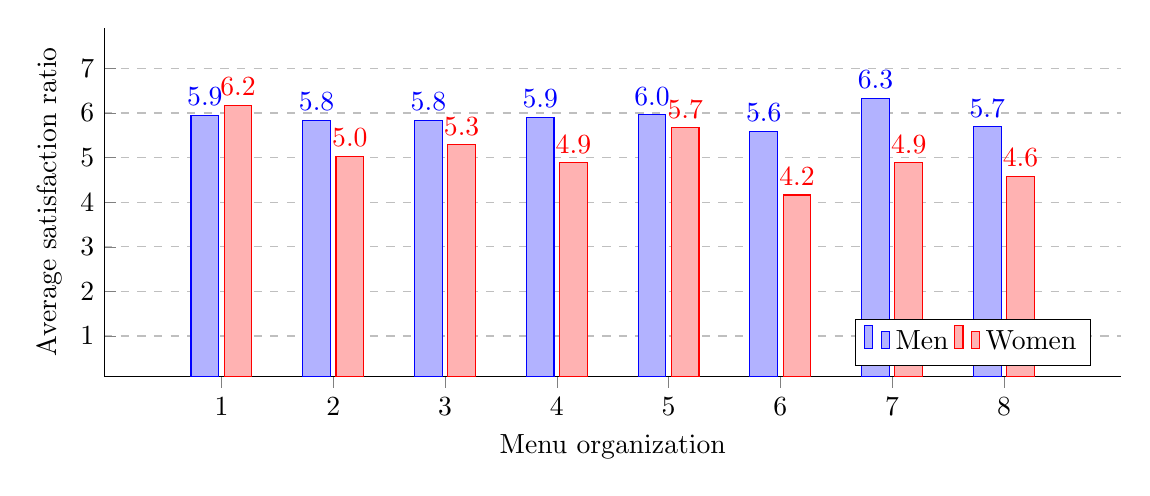
\begin{tikzpicture}
    \begin{axis}[
      %title={Evolution of student participation for each exercise},
      enlarge y limits=false,
      enlarge x limits=-1,
      height=6cm,
      width=14.5cm,
      axis lines*=left,
      xlabel={Menu organization},
      ylabel={Average satisfaction ratio},
      %xmin=1, xmax=4,
      ymin=1, ymax=7,
      xtick=data,
      ytick={1,2,3,4,5,6,7},
      legend pos=south east,
      legend columns=0,
      %xmajorgrids=true,
      ymajorgrids=true,
      grid style=dashed,
      enlargelimits=0.15,
      %histogram related :
      ybar,
      symbolic x coords={1,2,3,4,5,6,7,8},
      nodes near coords,
      every node near coord/.append style={
	  /pgf/number format/fixed zerofill,
	  /pgf/number format/precision=1
      }
      ]
      
    \addplot coordinates
    {(1,5.9375) (2,5.8333) (3,5.8333) (4,5.8958) (5,5.9583) (6,5.5833) 
     (7,6.3333) (8,5.6875)};
    \addplot coordinates
    {(1,6.1666) (2,5.0238) (3,5.2857) (4,4.8809) (5,5.6666) (6,4.16190) 
     (7,4.8809) (8,4.5714)};
    
    \legend{Men, Women}
    
    \end{axis}
  \end{tikzpicture}
  \caption{Average satisfaction ratio for each menu organization according to 
the gender distinction.}
    \label{fig:satisfaction_gender}
\end{figure}

At the end of the experiment, participants were asked to \textit{rank} the menu 
organizations in order of preference and such that a menu ranked at the first 
place was considered as the most preferred menu by the subject. Figure 
\ref{fig:rankings} depicts the average ranking received by each menu 
organization. The traditional (1) and responsive menus (5) were mostly 
preferred by the subjects of the experiment. The responsive minimised split 
menu (8) was by far the less preferred menu. It was ranked by 10 participants as 
the worst menu organization.

\begin{figure}[!ht]
    \centering
\begin{tikzpicture}
    \begin{axis}[
      %title={Evolution of student participation for each exercise},
      enlarge y limits=false,
      enlarge x limits=-1,
      height=6cm,
      width=14.5cm,
      axis lines*=left,
      xlabel={Menu organization},
      ylabel={Average ranking},
      %xmin=1, xmax=4,
      ymin=1, ymax=8,
      xtick=data,
      ytick={1,2,3,4,5,6,7,8},
      legend pos=east,
      legend columns=0,
      %xmajorgrids=true,
      ymajorgrids=true,
      grid style=dashed,
      enlargelimits=0.15,
      %histogram related :
      ybar,
      symbolic x coords={1,2,3,4,5,6,7,8},
      nodes near coords,
      ]
      
    \addplot[orange!70!black, fill=orange!30] coordinates
    {(1,2.7) (2,4.1) (3,4.2) (4,5.6) (5,2.9) (6,4.9) (7,4.9) (8,6.7)};
    
    %\legend{Men, Women}
    
    \end{axis}
  \end{tikzpicture}
  \caption{Average ranking received by each menu organization.}
    \label{fig:rankings}
\end{figure}

\section{Confirming, reversing and updating hypotheses}
The objective of the experiment was to confirm or reverse an initial set of 
11 hypotheses. The results analyzed in the previous sections have led us to 
undertake interesting observations. This section finally aims to confirm, 
reverse and update the initial assumptions based on these observations in order 
to conclude our study.

\subsection{Hypotheses and usability}
In the previous sections, we performed an in-depth analysis of 3 
usability-related properties: (1) effectiveness, (2) efficiency and (3) 
satisfaction. Effectiveness was measured by comparing the average error rate 
between the control condition menu and the new menu organizations. Therefore, 
this property will help us to confirm or reverse hypotheses based on the fact 
that some menu organizations may \textit{reduce the error rate}. The efficiency 
analysis was based on identifying \textit{selection time reduction} and 
eventually \textit{productivity enhancement}. Finally, user satisfaction was 
measured for and between each menu organization. It helped us to identify 
\textit{user preference} for some menu organizations.\newline

Selection time and user preference were already mentioned by the 11 initial 
hypotheses. Two types of hypothesis must now be added up to each 
menu organization. These assumptions are about error rate and productivity 
which were not taken into account at the beginning of our study. These 
additional hypotheses are formulated below:

\begin{itemize}
 \item \textbf{H1c:} the split menu reduces the error rate.
 \item \textbf{H1d:} the split menu enhances the productivity.
 \item \textbf{H2c:} the minimised menu reduces the error rate.
 \item \textbf{H2d:} the minimised menu enhances the productivity.
 \item \textbf{H3c:} the responsive menu reduces the error rate.
 \item \textbf{H3d:} the responsive menu enhances the productivity.
\end{itemize}


\subsection{Split menu}
In 1994, \textsc{Sears} and \textsc{Shneiderman} proved that split menu 
helped to reduce the selection time and received a greater user preference for 
desktop computer system. Unfortunately, our experiment based on 
mobile systems did not show promising results. During the experiment, the split 
menu provided the same average error rate than a traditional menu ($3.33\%$). 
It appears that it also slightly increased the average selection time ($2.52s$ 
instead of $2.5s$ for the control condition menu). Khalid 
\textsc{Al-Omar} and Dimitrios \textsc{Rigas} already experienced the 
same results with their small menu.\newline

In conclusion, the split menu does \textit{not} reduce the error rate, nor the 
selection time in the presence of a mobile system. It was also \textit{not} 
preferred over the traditional menu. Therefore, all the hypotheses based on the 
split menu have to be reversed.

\subsection{Minimised menu}
The minimised menu was meant to help users to identify the desired item 
quicker by reducing the number of displayed items. At first glance, the 
experiment showed promising results. Indeed, the minimised menu provided the 
second lowest average error rate with $0.56\%$ only. Unfortunately, this menu 
organization did not allow to reduce the selection time. The productivity of 
users was slightly increased but still remains unsignificant to be recognized. 
Finally, users were satisfied by the minimised menu organization but did not 
prefer it over the traditional menu.\newline

In conclusion, the minimised menu help users to reduce their error rate. 
However, it is not sufficient to reduce their selection time, nor their 
productivity, and it was not recognized as a preference. Therefore, we are 
only able to confirm one hypothesis:

\begin{itemize}
 \item \textbf{H2c:} the minimised menu reduces the error rate.
\end{itemize}

\subsection{Responsive menu}
Yusuke \textsc{Fukazawa} was the first researcher to publish results based on a 
a responsive menu organization. The idea was to adapt the menu organization to 
the small size of mobile screens. The responsive menu provided great results. 
First, the participants managed to achieve a $0\%$ average error rate by using 
this new 
menu organization. They also achieved the lowest average selection time and 
therefore, the highest productivity ratio. The responsive menu received the 
better satisfaction ratio along with the traditional menu and was preferred 
over all menu organizations.\newline

In conclusion, we managed to prove the 4 hypotheses formulated about responsive 
menus:

\begin{itemize}
 \item \textbf{H3a:} the responsive menu reduces the selection time.
 \item \textbf{H3b:} the responsive menu is preferred by users.
 \item \textbf{H3c:} the responsive menu reduces the error rate.
 \item \textbf{H3d:} the responsive menu enhances the productivity.
\end{itemize}

\subsection{Novice and master users}
Yusuke \textsc{Fukazawa} also noticed that novice and master users usually 
express different preferences regarding new menu organizations. Unfortunately, 
the participants of the experiment were mainly master and frequent smartphone 
users. Therefore, we can only prove the assumptions made on the master 
users and we have to dismiss the assumptions about the novices. Eventhough 
these frequent users expressed a great satisfaction to all menu organizations, 
they mainly ranked the traditional and responsive menus as their favorite 
ones.\newline

In conclusion, we can only confirm and update one hypothesis:

\begin{itemize}
 \item \textbf{H4b:} master users show a preference for the traditional and 
the responsive menus.
\end{itemize}

\subsection{Guidance informations and period of adjustment}
The survey paper was also used to gather users' thoughts about the guidance 
informations and the period of adjustment. There were 3 interesting sentences 
to analyze the impact of these notions on menu usability. Each sentence had to 
be rated on a scale ranging from 1 (disagree) to 7 (agree) for each menu 
organization. These sentences are listed below:

\begin{enumerate}
 \item I found this menu presented as expected.
 \item I needed to learn more this menu.
 \item I needed more guidance informations about this menu.
\end{enumerate}

The 1st and last sentences are helpful to assess the quality of the guidance 
informations provided at the beginning of each training session. Figure 
\ref{fig:guidance} depicts the average rating received for these sentences for 
each menu organization. According to these ratings, the subjects of the 
experiment were very satisfied by the quality of the guidance informations. 
They found menus were all organized as expected and guidance informations were 
sufficient for them to understand new menu organizations.\newline

During the experiment, the participants were first able to train themselves 
with each menu organization for 2 consecutive selections only. Then, they were 
asked if this period of adjustment was long enough according to them. The 
second sentence described above is interesting to evaluate this objective. 
Figure \ref{fig:period} depicts the average rating received for this sentence 
for each menu organization. The results are very prositive. Indeed, users have 
agreed to rate the period of adjustment long enough for all menu 
organizations.\newline

In conclusion, the guidance informations and the period of adjustment have been 
widely appreciated by the participants of the experiment. However we haven't 
tested the experiment without these notions. Therefore, we cannot take proper 
conclusions on the fact that they help users to handle a menu organization more 
efficiently. Since users appreciated the quantity and quality of the provided 
guidance informations, we can only prove the following hypothesis:

\begin{itemize}
 \item \textbf{H5a:} guidance informations help users to understand how a menu 
works.
\end{itemize}

\begin{figure}[!ht]
    
  \begin{subfigure}[t]{.49\textwidth}
  \centering
  \resizebox{\linewidth}{!}{
  \begin{tikzpicture}[baseline]
    \begin{axis}[
      %title={Evolution of student participation for each exercise},
      enlarge y limits=false,
      axis lines*=left,
      xlabel={Menu organization},
      ylabel={Average rating},
      xmin=1, xmax=8,
      ymin=1, ymax=7,
      xtick=data,
      ytick={1,2,3,4,5,6,7},
      legend pos=east,
      legend columns=0,
      %xmajorgrids=true,
      ymajorgrids=true,
      grid style=dashed,
      enlargelimits=0.15,
      %histogram related :
      ybar,
      symbolic x coords={1,2,3,4,5,6,7,8},
      nodes near coords,
      ]
      
    \addplot[orange!70!black, fill=orange!30] coordinates
    {(1,6.7) (2,6.7) (3,6.7) (4,6.5) (5,6.6) (6,6.6) (7,6.7) 
     (8,6.6)};
    
    %\legend{Men, Women}
    
    \end{axis}
  \end{tikzpicture}}
  \caption{Average rating gathered for the sentence \enquote{I found this menu 
presented as expected} for each menu organization.}
  \label{fig:background}
  \end{subfigure}
  \begin{subfigure}[t]{.49\textwidth}
    \resizebox{\linewidth}{!}{
    \centering
    \begin{tikzpicture}[baseline]
    \begin{axis}[
      %title={Evolution of student participation for each exercise},
      enlarge y limits=false,
      axis lines*=left,
      xlabel={Menu organization},
      ylabel={Average rating},
      xmin=1, xmax=8,
      ymin=1, ymax=7,
      xtick=data,
      ytick={1,2,3,4,5,6,7},
      legend pos=east,
      legend columns=0,
      %xmajorgrids=true,
      ymajorgrids=true,
      grid style=dashed,
      enlargelimits=0.15,
      %histogram related :
      ybar,
      symbolic x coords={1,2,3,4,5,6,7,8},
      nodes near coords,
      every node near coord/.append style={
	  /pgf/number format/fixed zerofill,
	  /pgf/number format/precision=1
      }
      ]
      
    \addplot[orange!70!black, fill=orange!30] coordinates
    {(1,1.1) (2,1.6) (3,1.4) (4,1.4) (5,1.3) (6,1.3) (7,1.2) (8,1.3)};
    
    %\legend{Men, Women}
    
    \end{axis}
  \end{tikzpicture}}
  \caption{Average rating gathered for the sentence \enquote{I needed more 
guidance informations about this menu} for each menu organization.}
  \end{subfigure}
  \caption{}
    \label{fig:guidance}
\end{figure}

\begin{figure}[!ht]
    \centering
\begin{tikzpicture}
    \begin{axis}[
      %title={Evolution of student participation for each exercise},
      enlarge y limits=false,
      enlarge x limits=-1,
      height=6cm,
      width=14.5cm,
      axis lines*=left,
      xlabel={Menu organization},
      ylabel={Average rating},
      %xmin=1, xmax=4,
      ymin=1, ymax=7,
      xtick=data,
      ytick={1,2,3,4,5,6,7},
      legend pos=east,
      legend columns=0,
      %xmajorgrids=true,
      ymajorgrids=true,
      grid style=dashed,
      enlargelimits=0.15,
      %histogram related :
      ybar,
      symbolic x coords={1,2,3,4,5,6,7,8},
      nodes near coords,
      ]
      
    \addplot[orange!70!black, fill=orange!40] coordinates
    {(1,1.1) (2,1.4) (3,1.4) (4,1.4) (5,1.3) (6,1.3) (7,1.2) (8,1.3)};
    
    %\legend{Men, Women}
    
    \end{axis}
  \end{tikzpicture}
  \caption{Average rating gathered for the sentence \enquote{I needed to learn 
more this menu} for each menu organization.}
    \label{fig:period}
\end{figure}

\subsection{Mixed-initiative menus}
The experiment was also set up with 3 mixed-initiative menus which combined 
split, responsive and/or minimised properties. The idea was to implement 
complementary menu organizations and benefit from their respective advantages. 
The first results were encouraging as all these mixed-initiative menus 
provided a lower average error rate. The minimised responsive split menu even 
provided the second lowest average error rate with $0.56\%$. Moreover, these 
new menu organizations provided a lower average selection time and thus 
enhanced users' productivity. Unfortunately these mixed-initiative menus did 
not sufficiently satisfied the subjects of the experiment. The minimised 
responsive split menu was even ranked 10 times as the worst menu organization in 
terms of user preference.\newline

In conclusion, we can add and confirm the following hypotheses to our study:

\begin{itemize}
 \item \textbf{H6a:} the minimised split menu reduces the error rate.
 \item \textbf{H6b:} the minimised split menu reduces the selection time.
 \item \textbf{H6c:} the minimised split menu enhances the 
productivity.\newline
 \item \textbf{H7a:} the responsive split menu reduces the error rate.
 \item \textbf{H7b:} the responsive split menu reduces the selection time.
 \item \textbf{H7c:} the responsive split menu enhances the 
productivity.\newline
 \item \textbf{H8a:} the minimised responsive menu reduces the error rate.
 \item \textbf{H8b:} the minimised responsive menu reduces the selection time.
 \item \textbf{H8c:} the minimised responsive menu enhances the 
productivity.\newline
 \item \textbf{H9a:} the minimised responsive split menu reduces the error 
rate.
 \item \textbf{H9b:} the minimised responsive split menu reduces the selection 
time.
 \item \textbf{H9c:} the minimised responsive split menu enhances the 
productivity.
\end{itemize}

\chapter{Conclusion}
Conceiving, designing and testing new menu organizations was a long and tough 
task. First, it was necessary to understand and summarize previous researches. 
It was an essential step to extract the currently available knowledge about 
menu usability. Then, it was essential to formulate an initial set of 
hypotheses in order to guide the development of the experimental method. 
Based on these assumptions and this method, an Android application was 
implemented to conduct the experiment and results were extracted from it. After 
a torough analysis of these results, we were finally able to confirm, reverse 
and update our hypotheses.\newline

The experimental method set up during the study helped us to confirm many 
assumptions. First, we observed that all new menu organizations were beneficial 
in reducing the average error rate, except for the split menu that provided 
the same error rate as the traditional menu. Then, we proved that the 
responsive and the 4 mixed-initiative menus helped users to reduce their average 
selection time and enhance their productivity. Moreover, users showed a higher 
preference rate for the responsive and the traditional menus. Finally, we 
have shown that guidance informations can help users to understand the overal 
operation of a menu organization.\newline

In conclusion, the split menu organization developed by \textsc{Sears} and 
\textsc{Shneiderman} is not the ideal solution for smartphone resolutions. The 
traditional and responsive menus received the highest user preference. The 
responsive menu also proved to be the most performant one in terms of 
usability. Therefore, the responsive menu designed by Yusuke \textsc{Fukazawa} 
with a specific focus towards small touch screens appears to be the most 
promising menu organization for smartphones. Further experiments should focus 
on this novative menu organization.

\section{Further}
Some matters remain unchallenged at the end of this study. Further 
improvements and additional issues remain to be accomplished, improved and 
set to keep enhancing our knowledge base about HCI and menu usability. This 
section aims to enumerate some of these matters.

\begin{itemize}
 \item \textbf{Large menu}: according to Khalid \textsc{Al-Omar} and Dimitrios 
\textsc{Rigas}, our set of menu items should be considered as a \enquote{small 
menu}. They tested new menu organizations with both a small set of 17 items and 
a larger set of 29 items. During their controlled experiment, they identified 
varying preferences between these menus. Therefore, the responsive menu may not 
be the ideal solution with larger menus.
 \item \textbf{Hot list}: according to \textsc{Sears} and 
\textsc{Shneiderman}, the hot list of a split menu should not exceed 4 items. 
During the experiment, we decided to implement a hot list made of 3 items. A 
split menu organization displaying a different hot list length may eventually 
be preferred by users and/or enhance their productivity.
 \item \textbf{Learning effect}: some subjects of the experiment were concerned 
about the learning effect between each session. Indeed, a few ones recognized 
to know the items better after a few evaluation sessions. Therefore, the 
final results may include some sort of bias.
 \item \textbf{Evaluation session}: some menu organizations are now 
acknowledged to be more usable than other ones with smartphones. We should 
conduct a second experiment which targets specifically these menu organizations 
and offers longer evaluation sessions. Indeed, a set of 10 selections for 
each menu seems like a short session in comparison to previous studies.
 \item \textbf{Keystroke menu}: during our research, we implemented another 
type of menu organization called \enquote{keystroke}. It consists of a 
traditional menu overhung with a search bar. This feature allows users 
to type the name of the desired item and watch the menu updated in real time. 
Unfortunately, the conducted experiment was already quite long and we decided 
to set aside this menu organization.
 \item \textbf{Log file}: a final improvement to the Android application would 
be to store each user's actions in a log file for a deeper analysis of their 
behaviours with new menu organizations.
\end{itemize}

\chapter{Abbreviations}
\begin{description}
  \item[HCI]: Human-Computer Interaction.
  \item[IT]: Information Technology.
  \item[LSM]: Louvain School of Management.
  \item[UCL]: Université Catholique de Louvain.
  \item[UI]: User Interface.
  \item[UX]: User Experience.
\end{description}

\bibliographystyle{unsrt}
\nocite{*}
\bibliography{bibliography}
\addcontentsline{toc}{chapter}{Bibliography}

\appendix

\chapter{Survey} \label{survey}
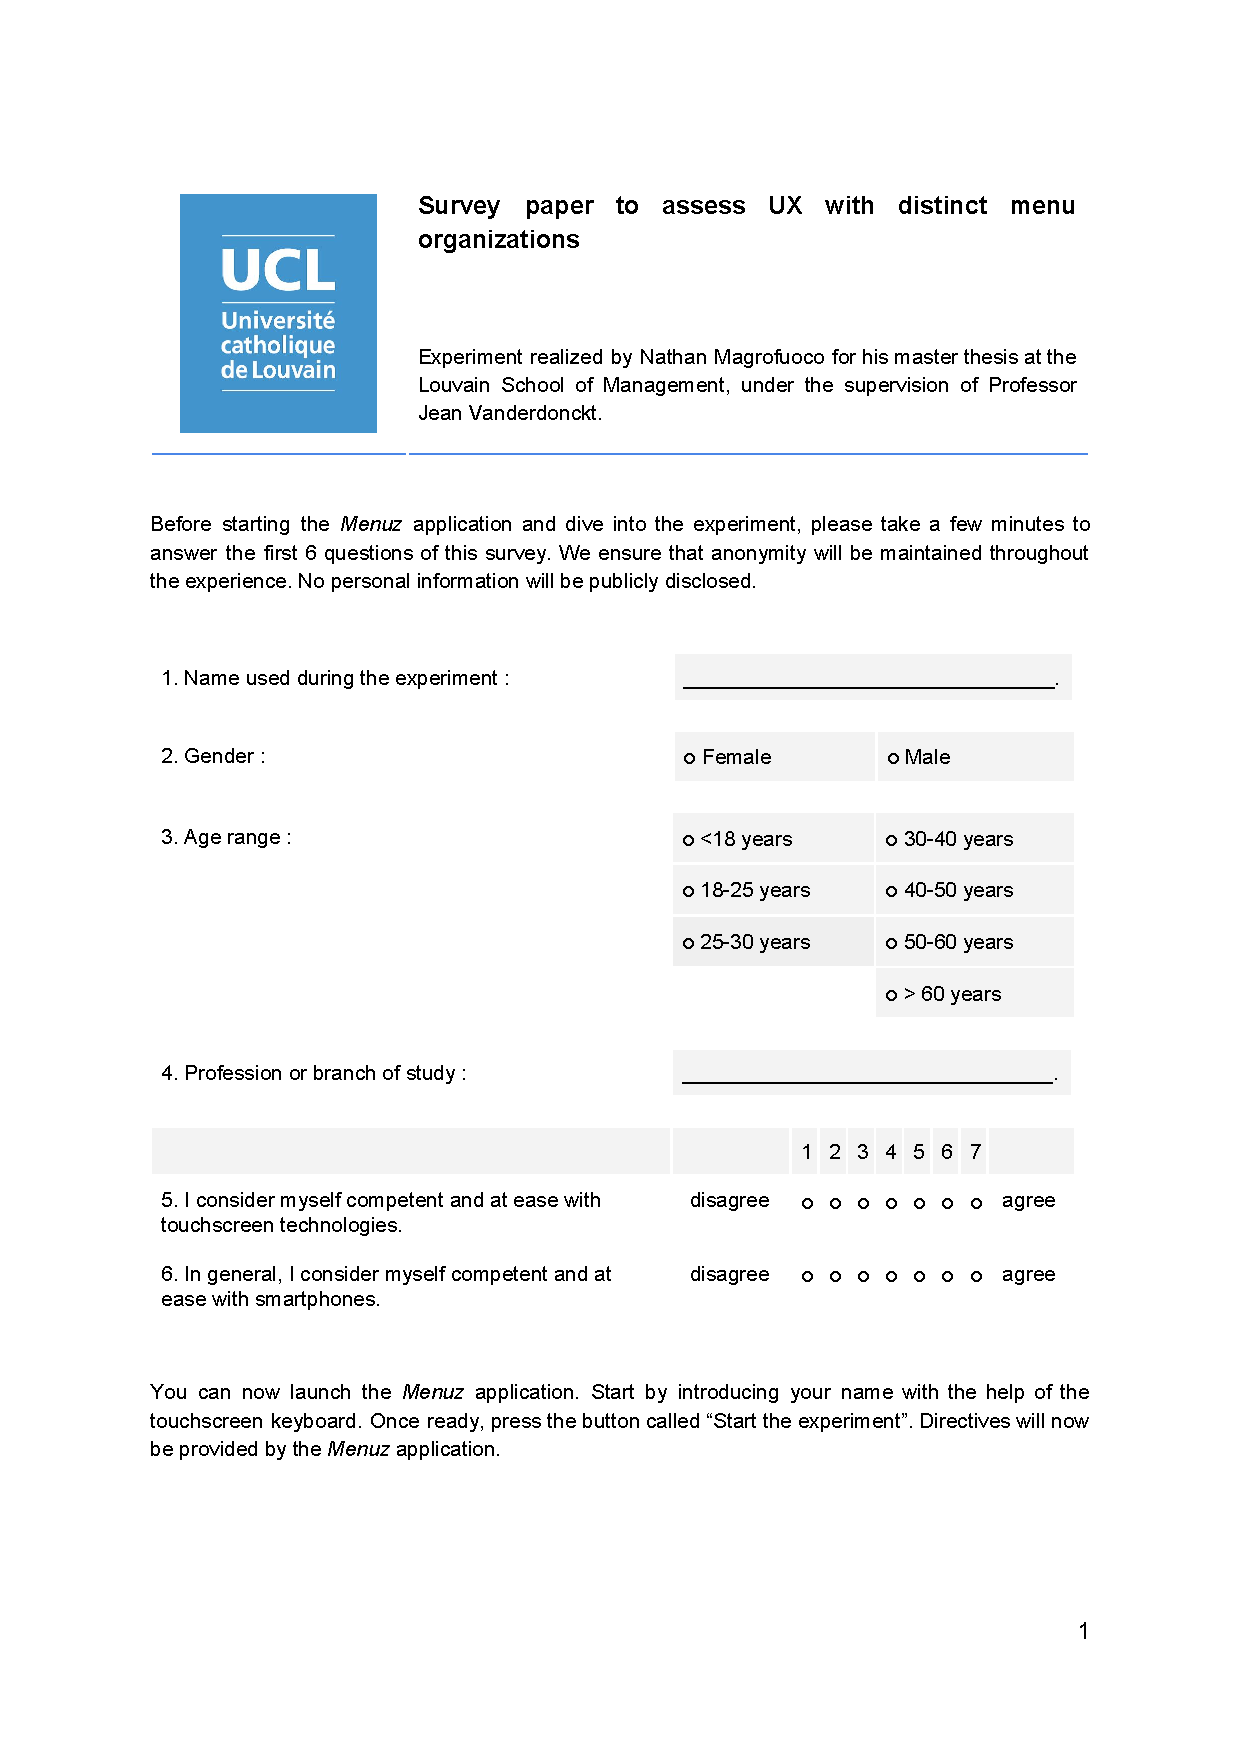
\includepdf[pages={1-},scale=0.85]{img/survey.pdf}

\chapter{Application UI} \label{screenshots}

\newpage

\begin{figure}[!ht]
  \begin{center}
    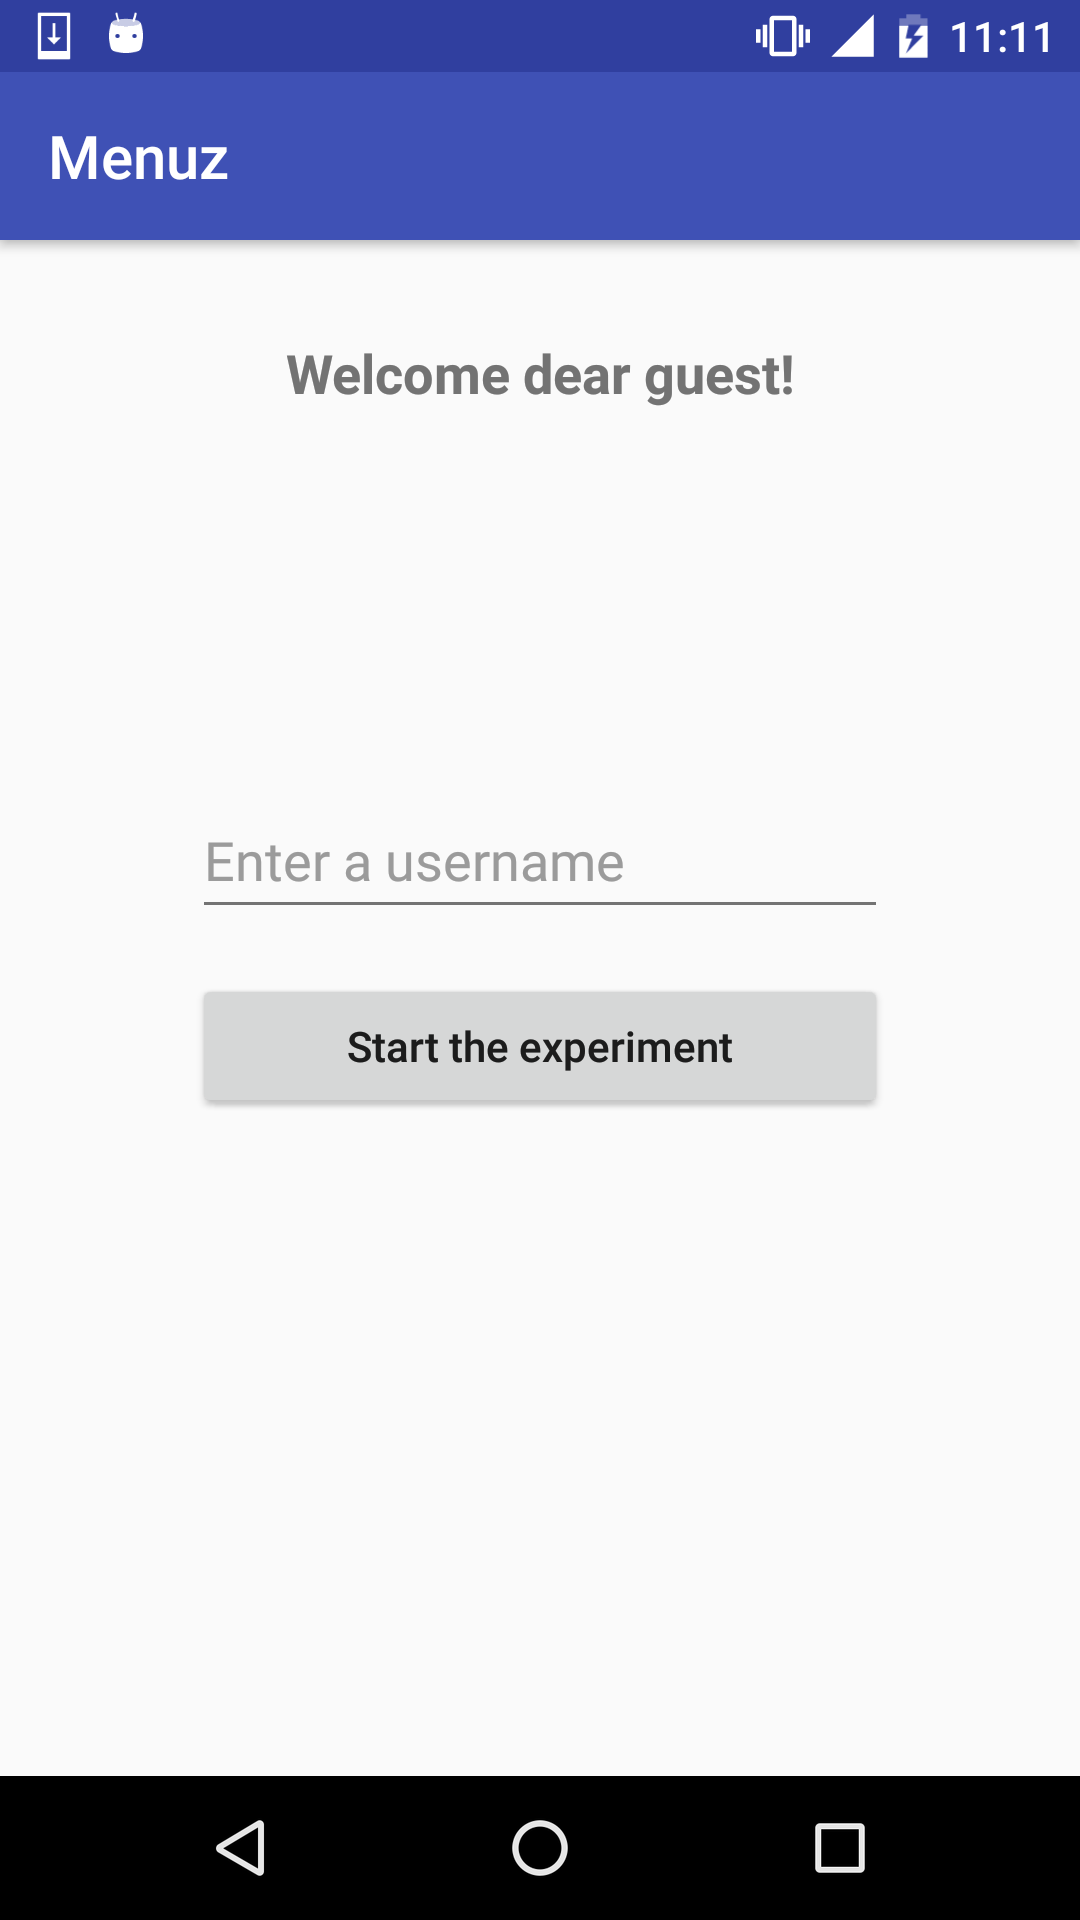
\includegraphics[scale=0.22]{img/main_activity.png}
    \label{fig:main_activity}
    \caption{MainActivity.}
  \end{center}
\end{figure}

\newpage

\begin{figure}[!ht]
  \begin{center}
    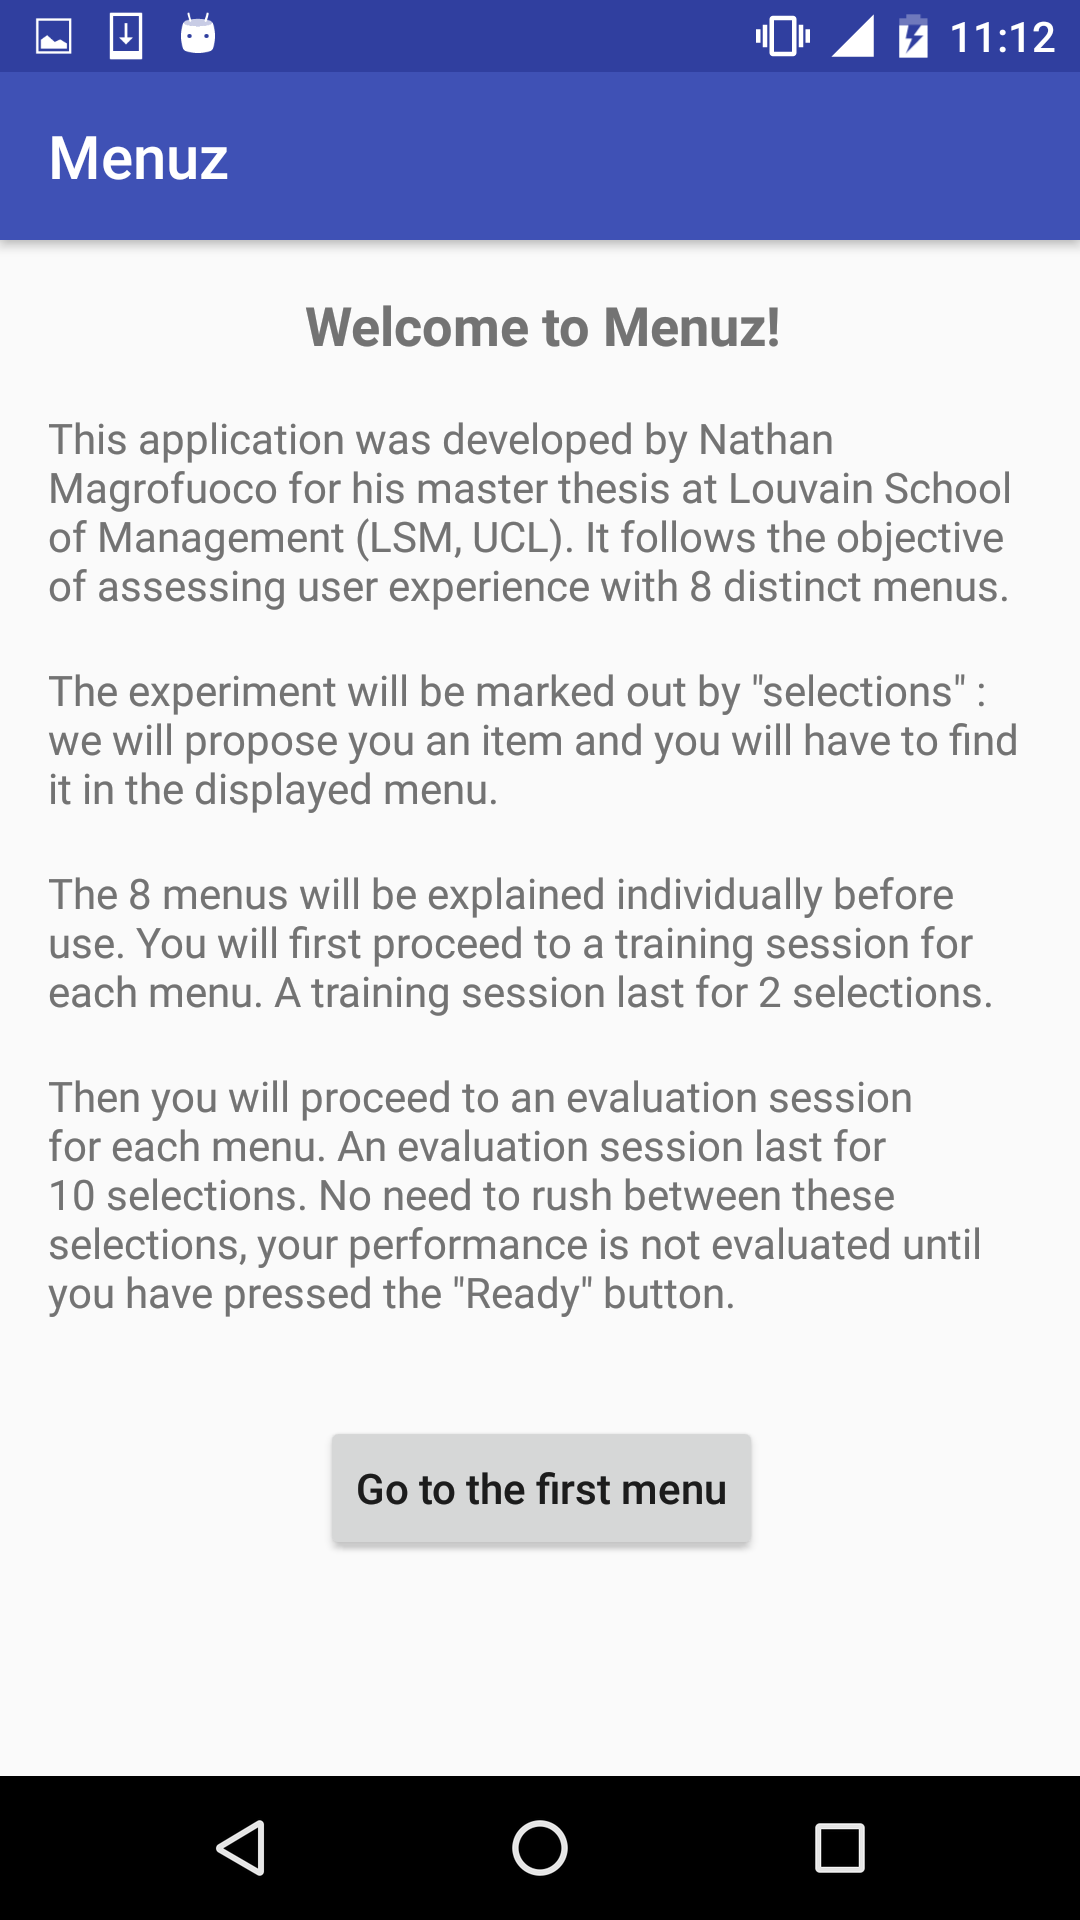
\includegraphics[scale=0.22]{img/intro_activity.png}
    \label{fig:intro_activity}
    \caption{IntroductionActivity.}
  \end{center}
\end{figure}

\newpage

\begin{figure}[!ht]
  \begin{center}
    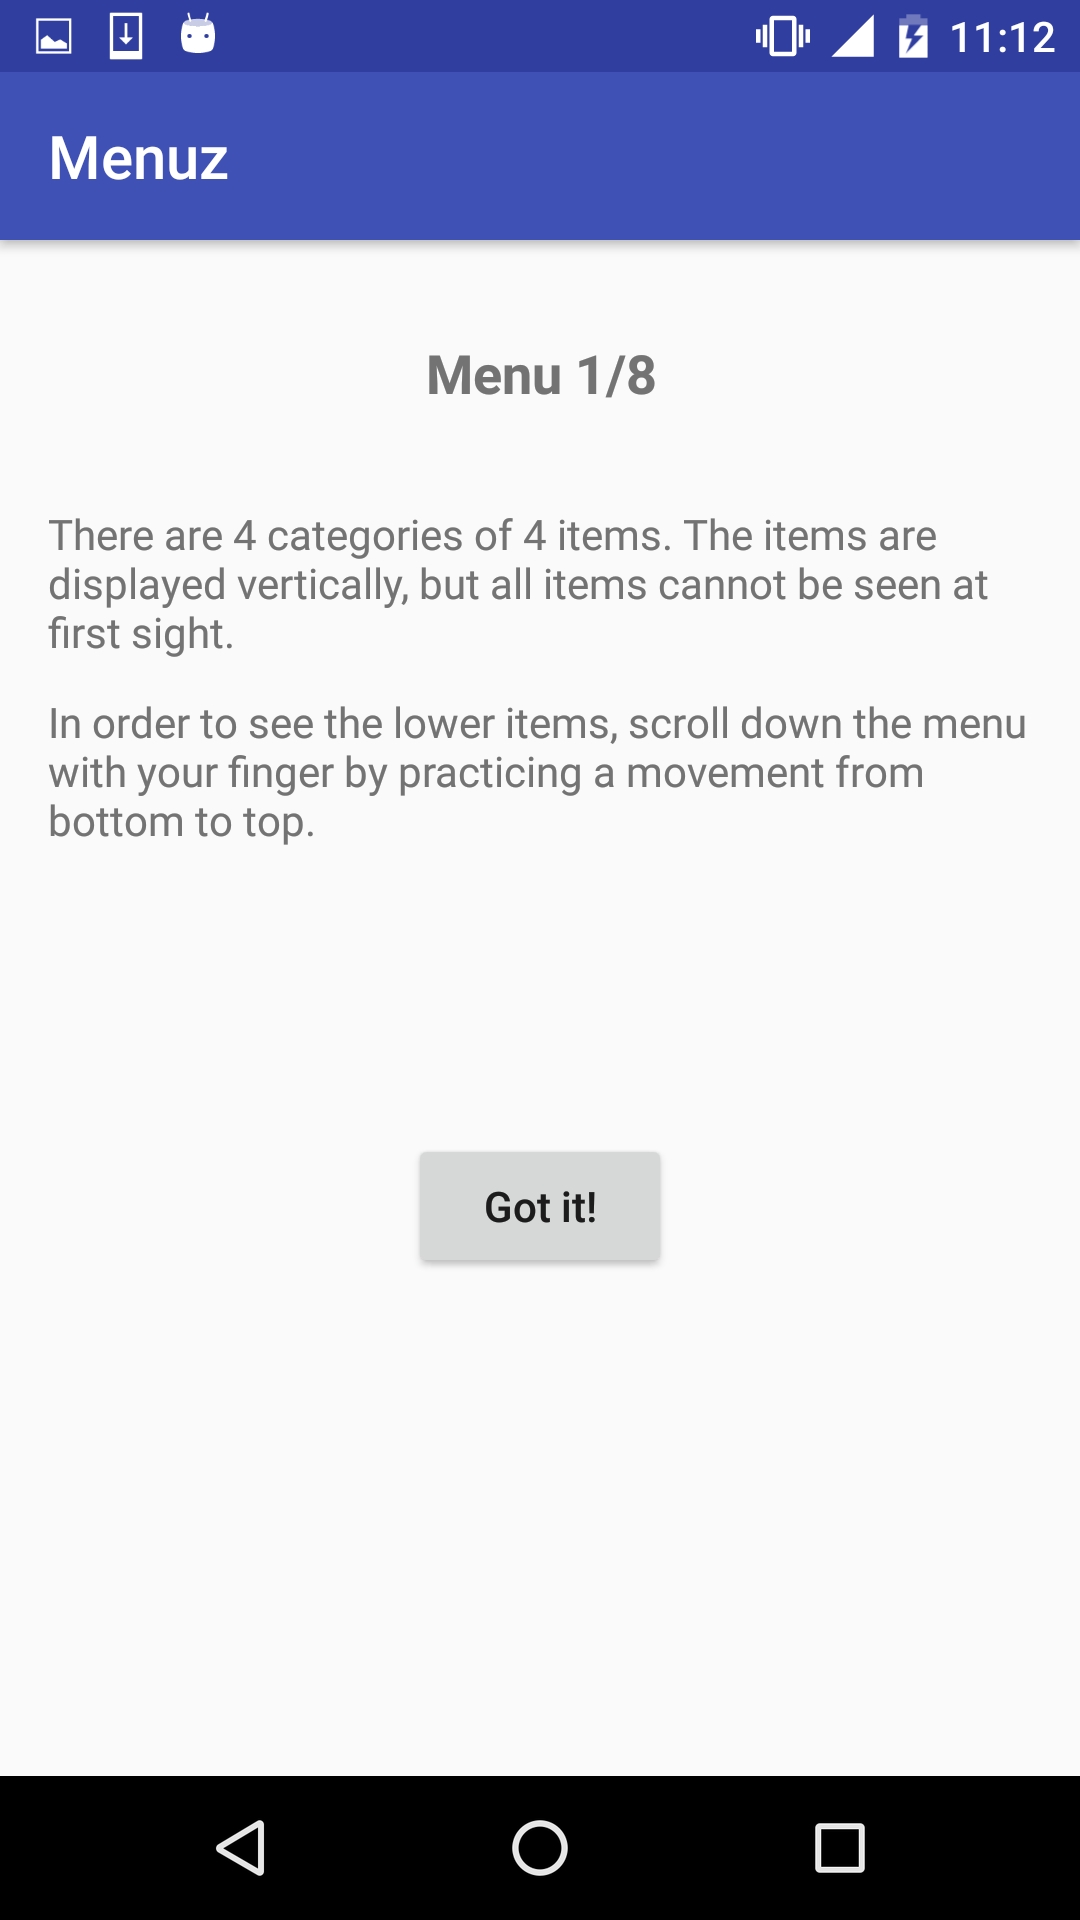
\includegraphics[scale=0.22]{img/menuintro_activity.png}
    \label{fig:menuintro_activity}
    \caption{MenuIntroductionActivity, before the 1st training session.}
  \end{center}
\end{figure}

\newpage

\begin{figure}[!ht]
  \begin{center}
    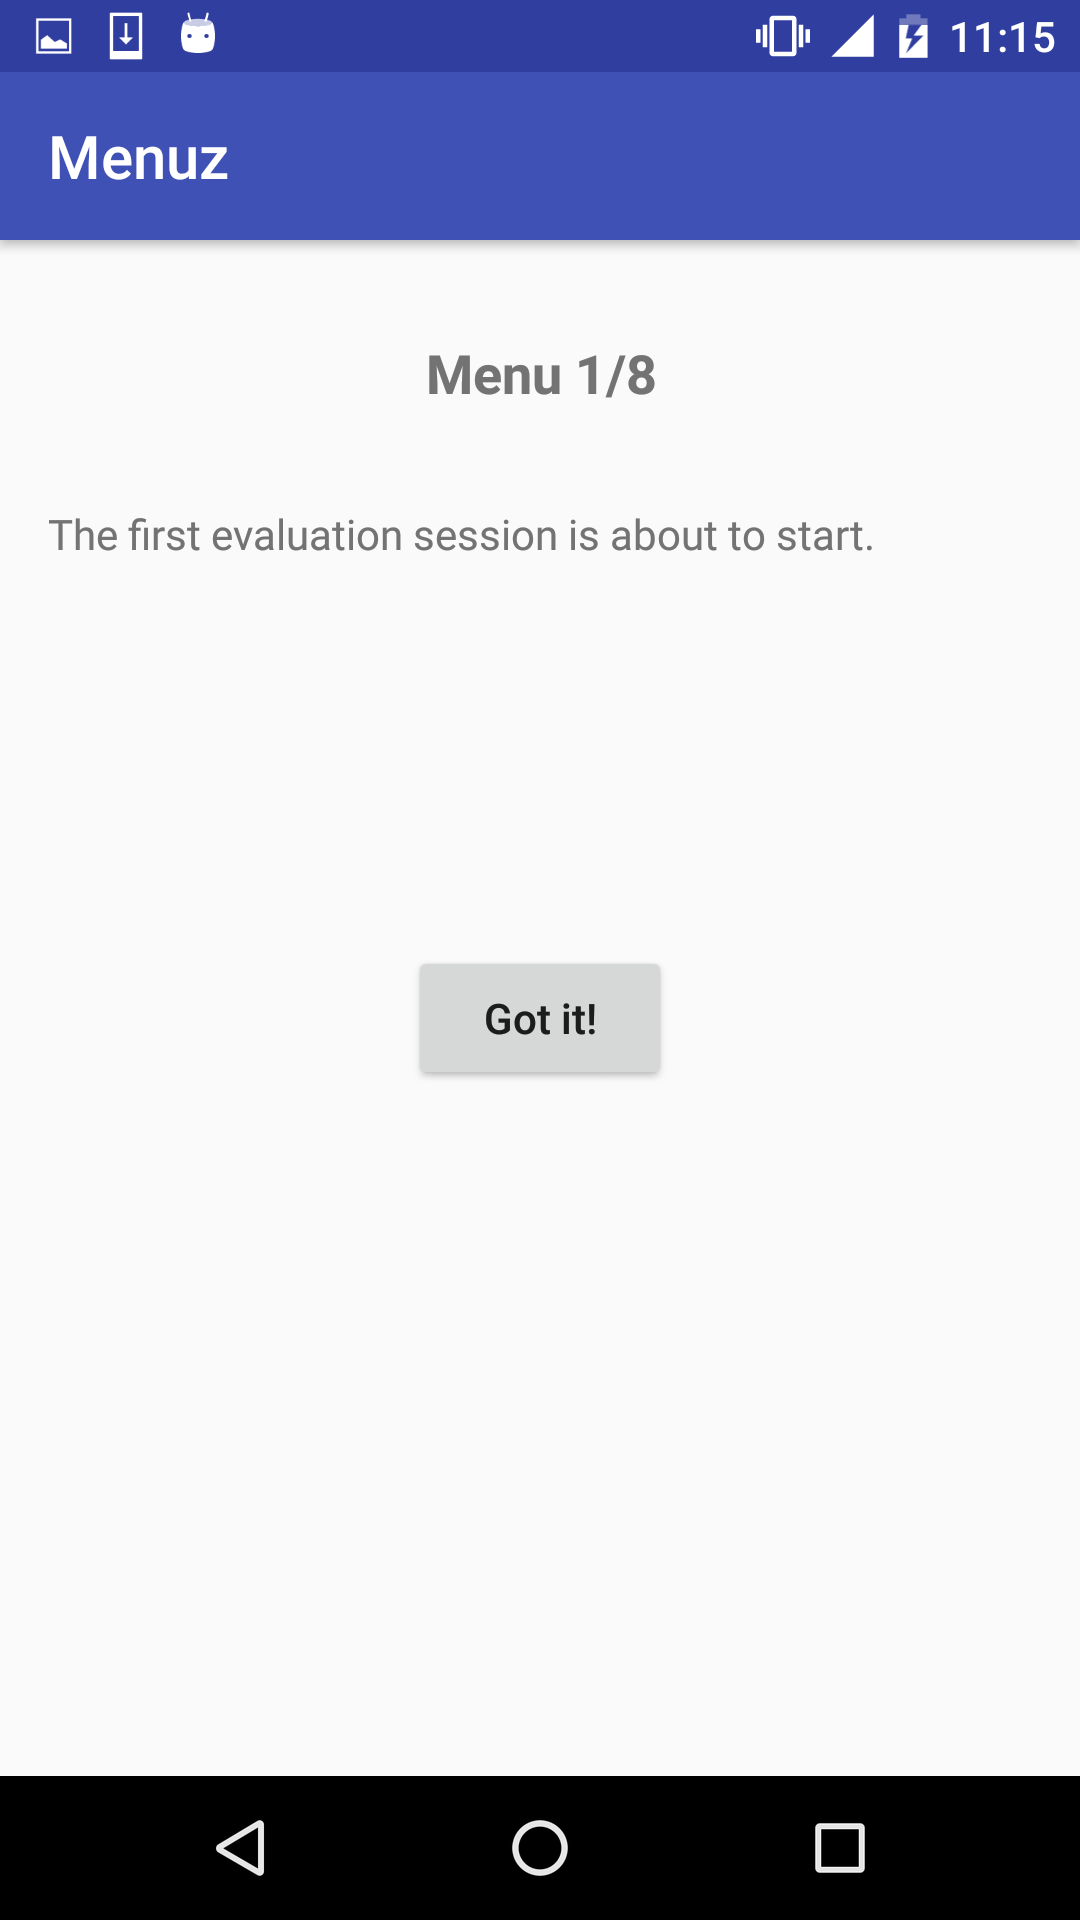
\includegraphics[scale=0.22]{img/menuintro_activityb.png}
    \label{fig:menuintro_activityb}
    \caption{MenuIntroductionActivity, before the 1st evaluation session.}
  \end{center}
\end{figure}

\newpage

\begin{figure}[!ht]
  \begin{center}
    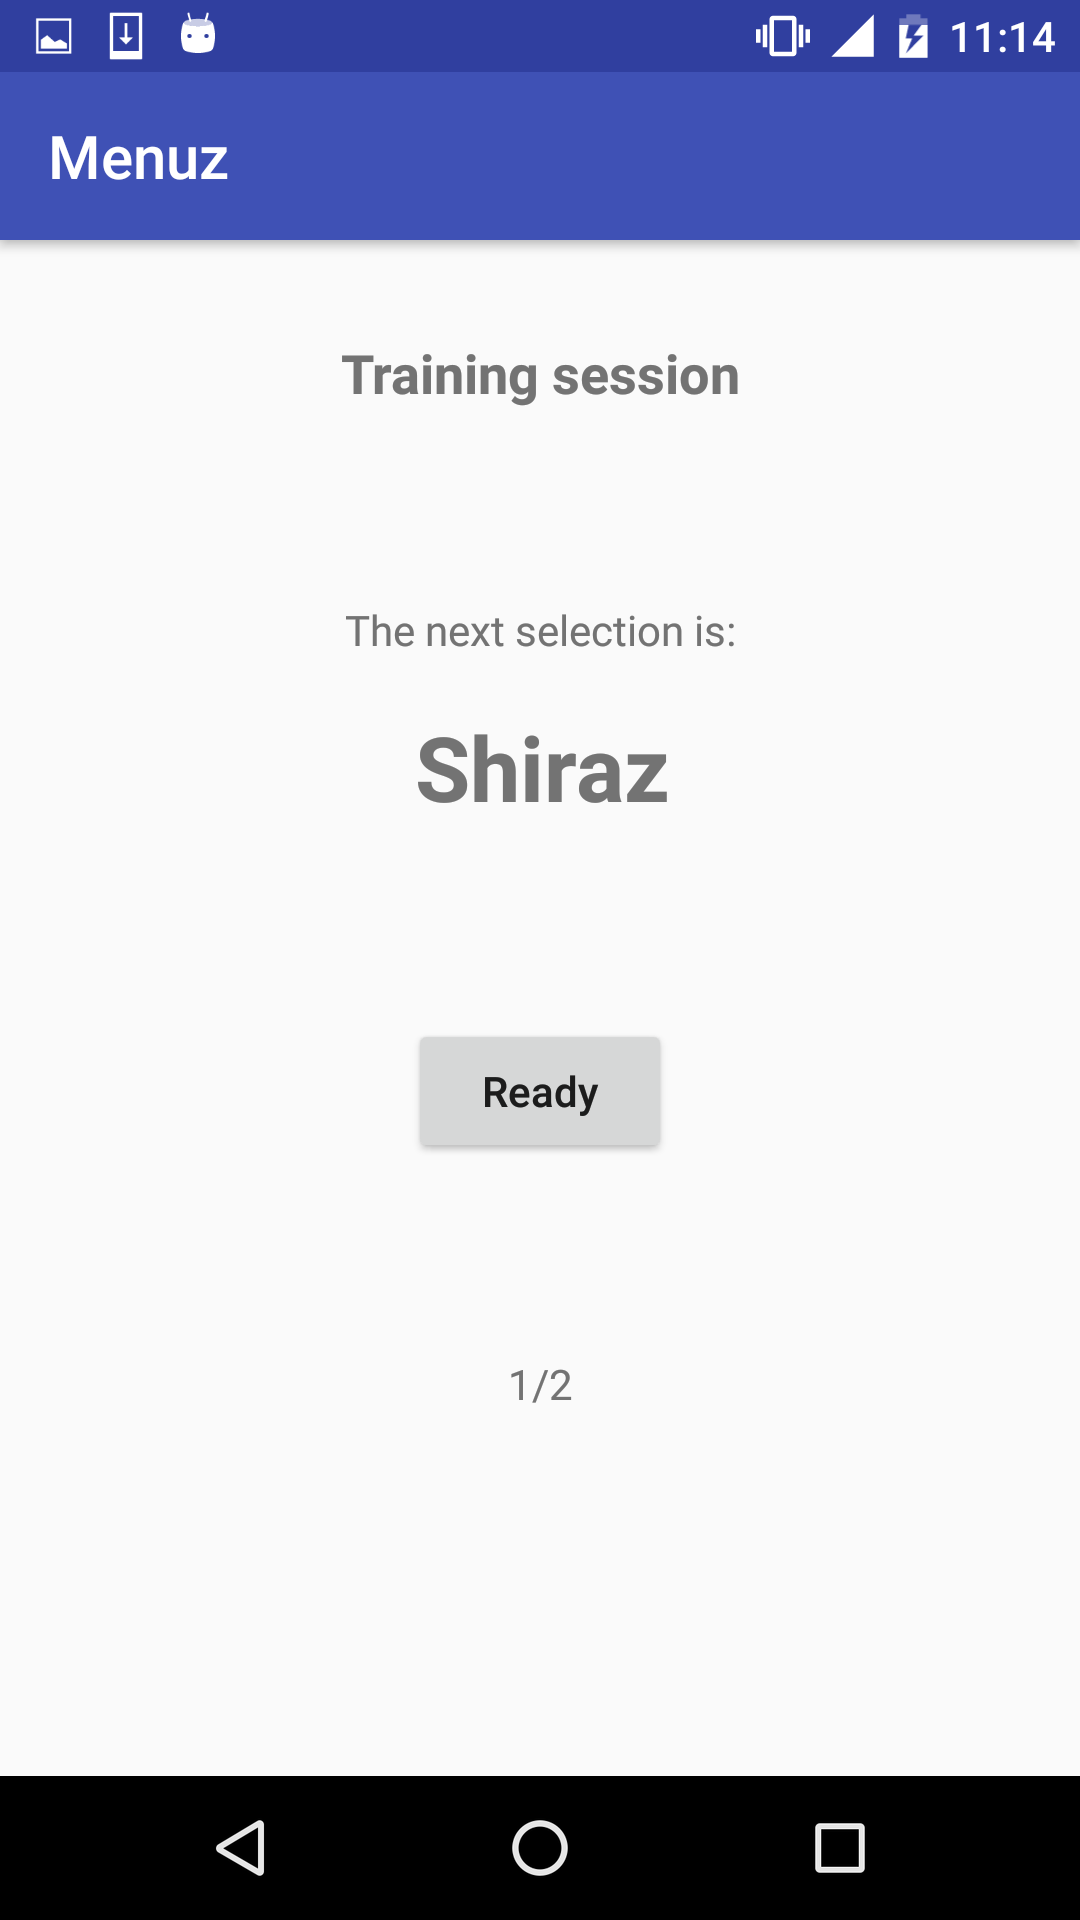
\includegraphics[scale=0.22]{img/nextselect_activity.png}
    \label{fig:nextselect_activity}
    \caption{NextSelectionActivity, during a training session.}
  \end{center}
\end{figure}

\newpage

\begin{figure}[!ht]
  \begin{center}
    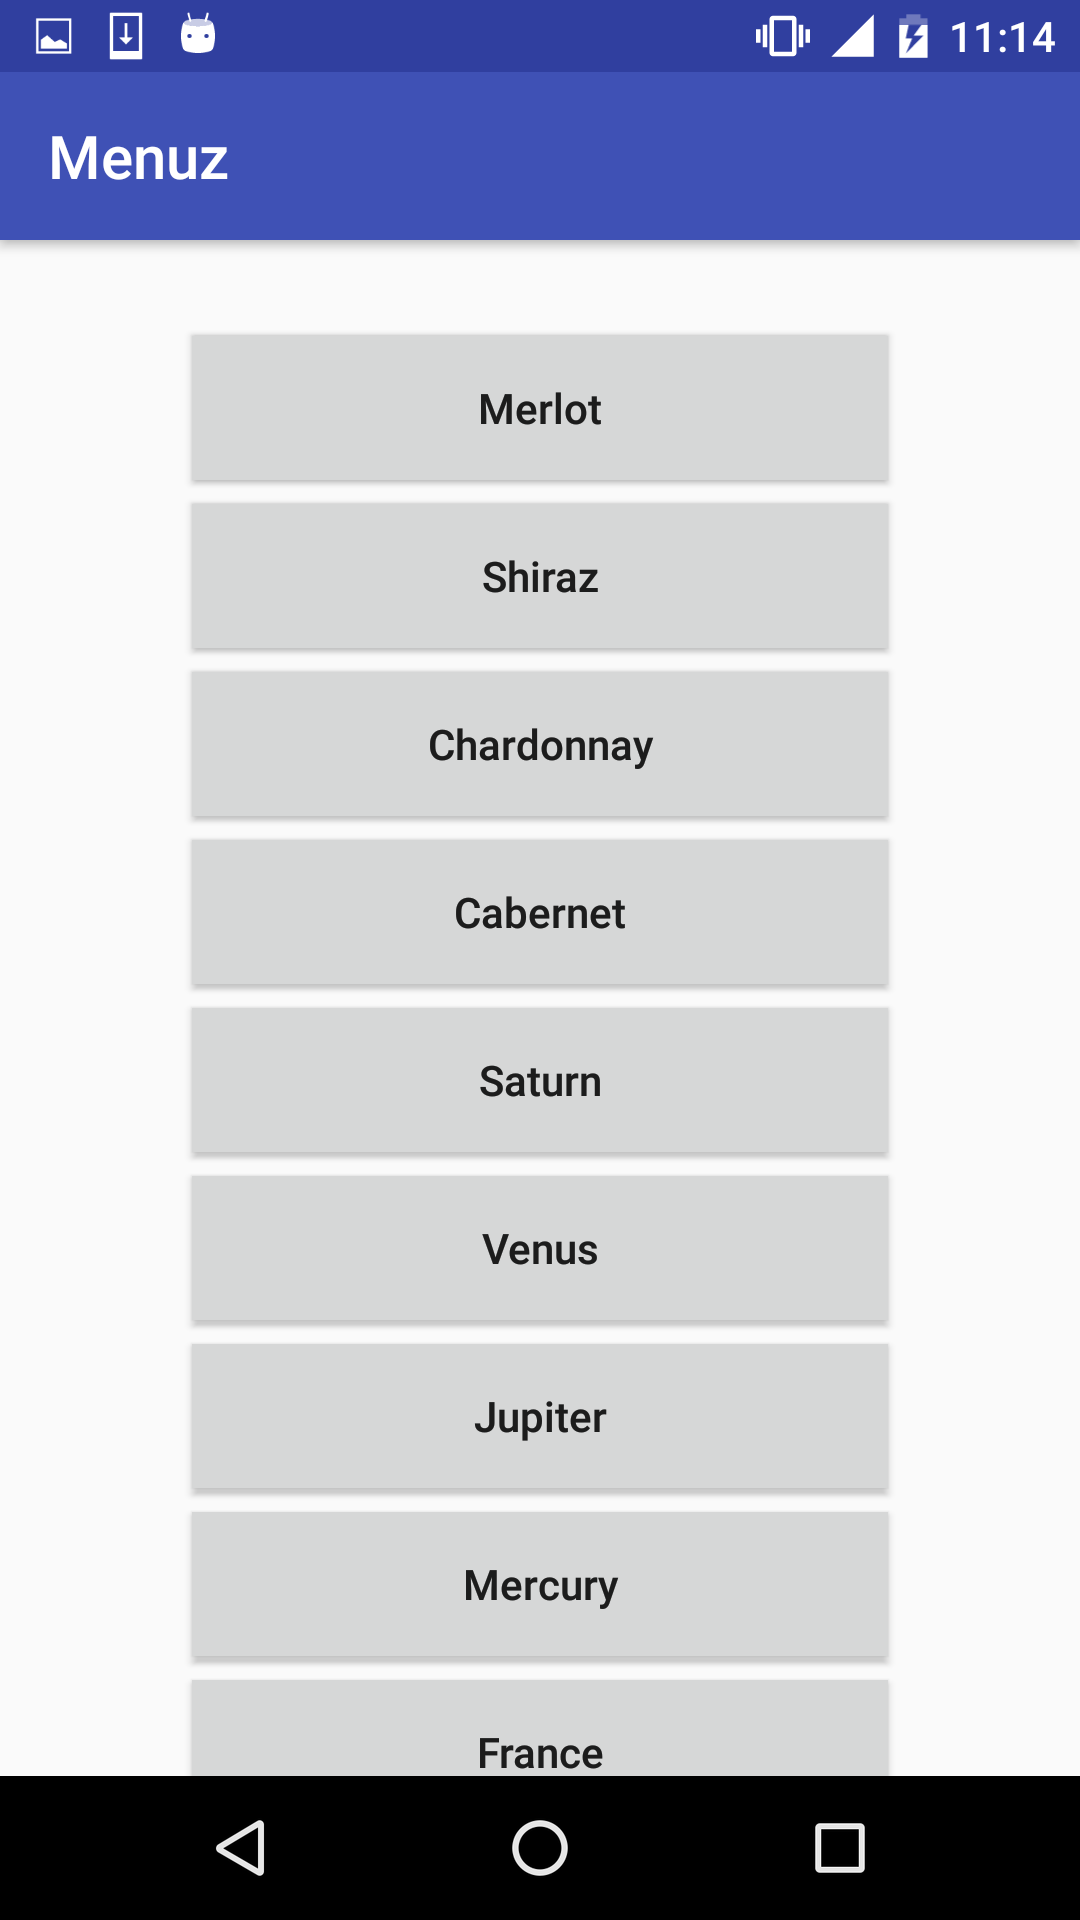
\includegraphics[scale=0.22]{img/menu.png}
    \label{fig:menu}
    \caption{MenuActivity.}
  \end{center}
\end{figure}

\newpage

\begin{figure}[!ht]
  \begin{center}
    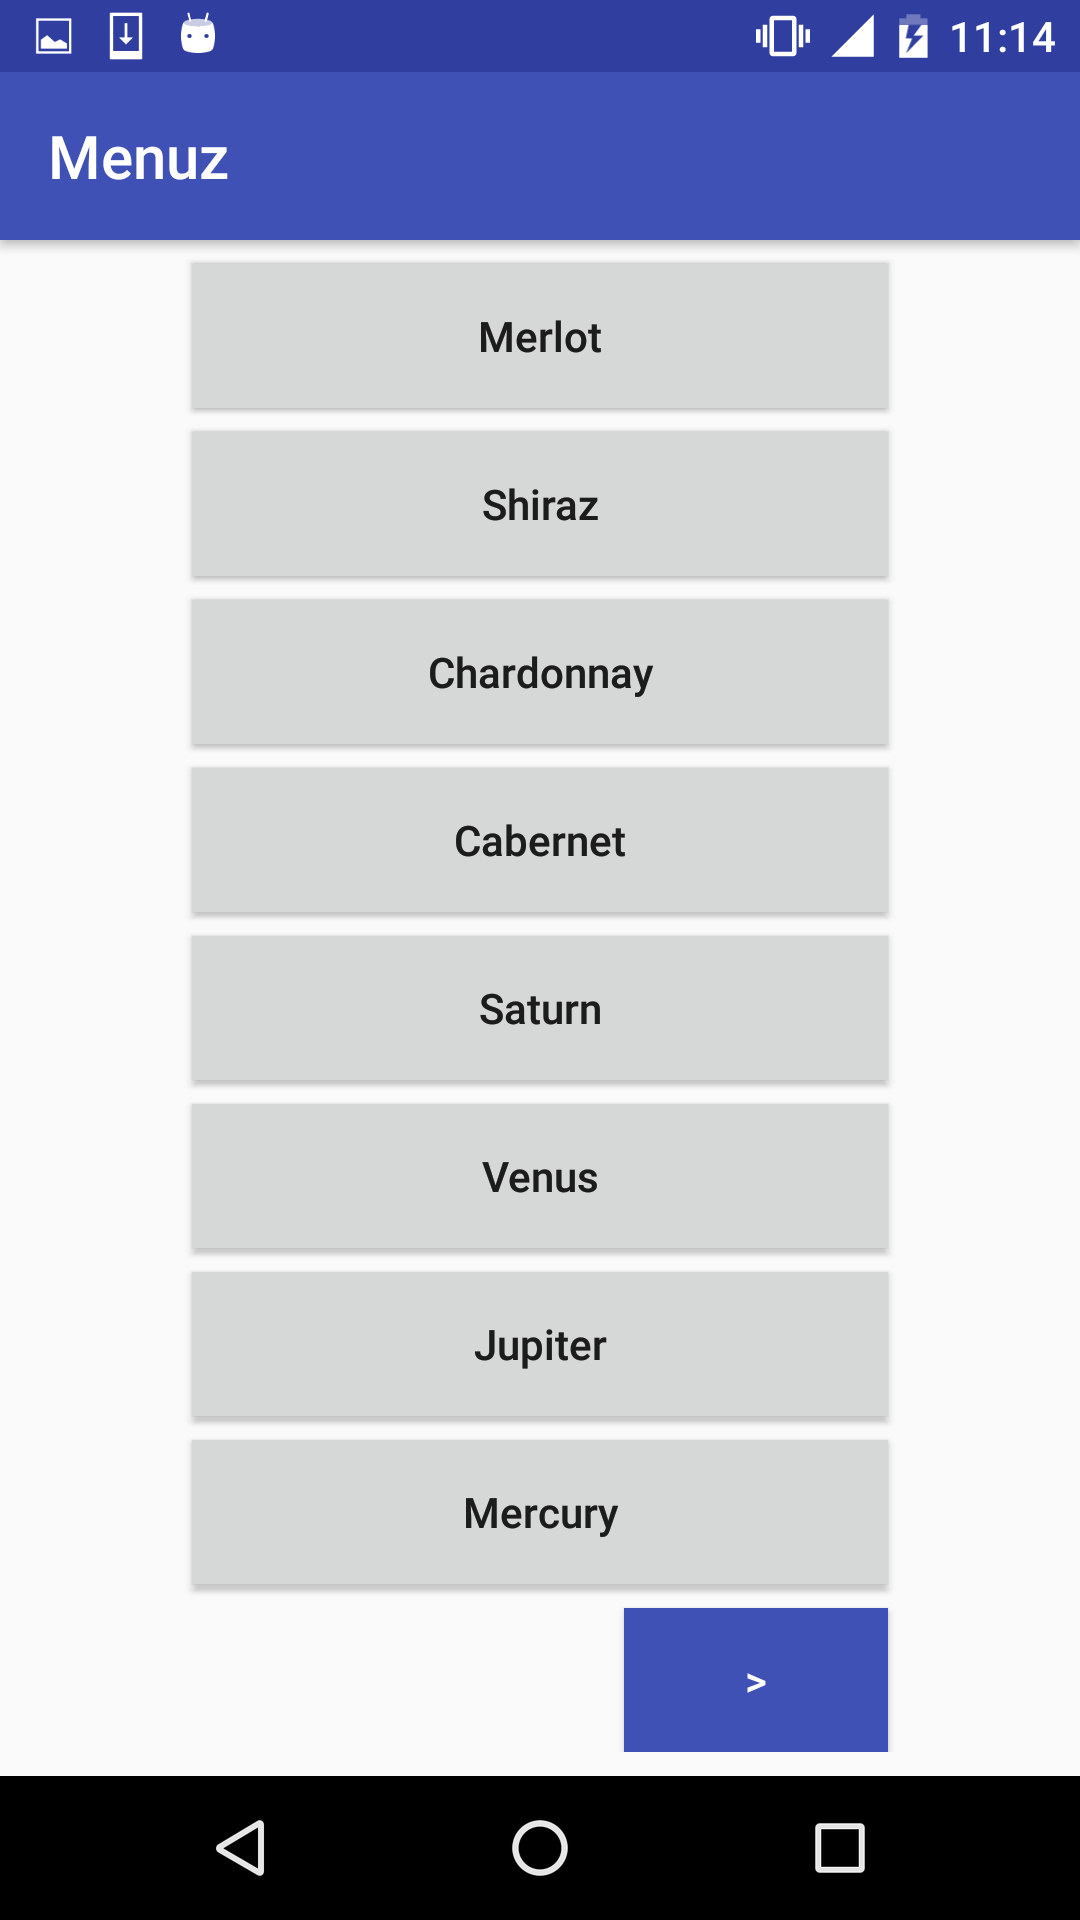
\includegraphics[scale=0.22]{img/mini_menu.png}
    \label{fig:mini_menu}
    \caption{MinimisedMenuActivity.}
  \end{center}
\end{figure}

\newpage

\begin{figure}[!ht]
  \begin{center}
    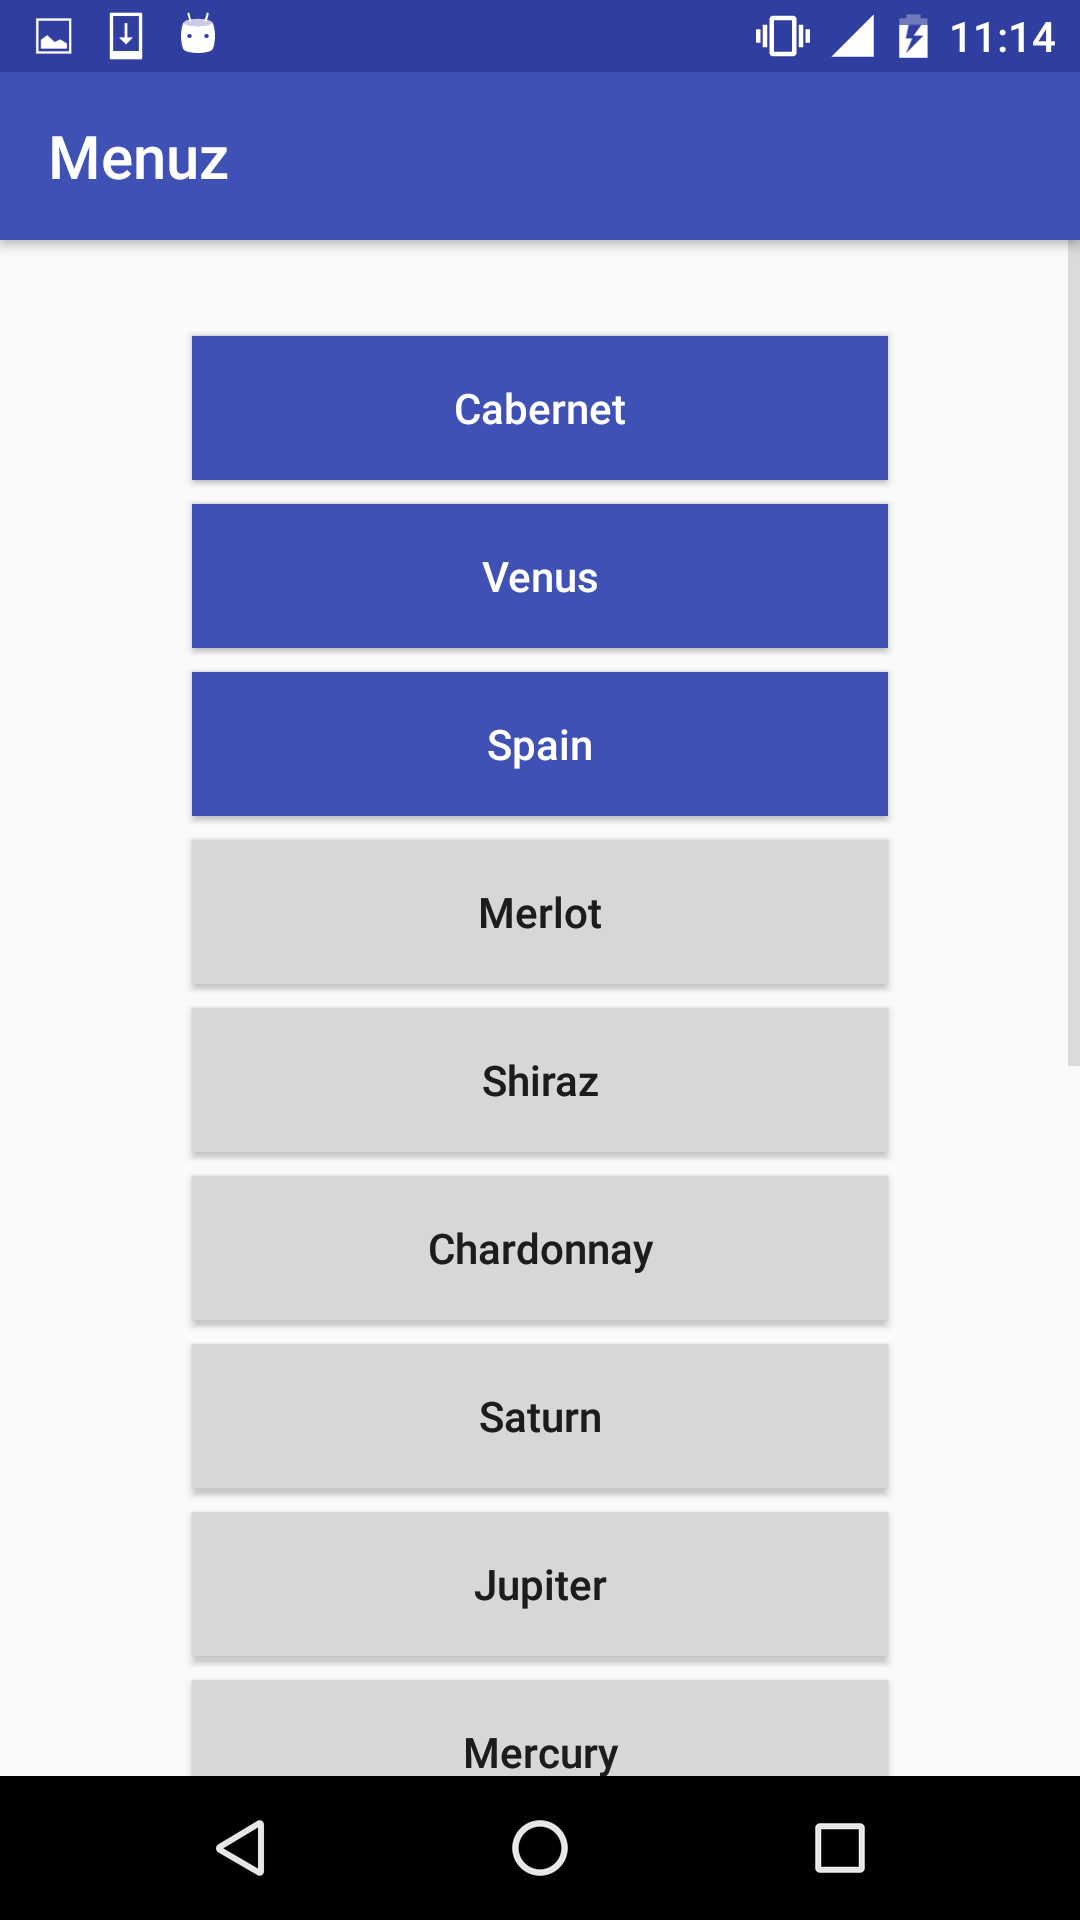
\includegraphics[scale=0.22]{img/split_menu.png}
    \label{fig:split_menu}
    \caption{SplitMenuActivity.}
  \end{center}
\end{figure}

\newpage

\begin{figure}[!ht]
  \begin{center}
    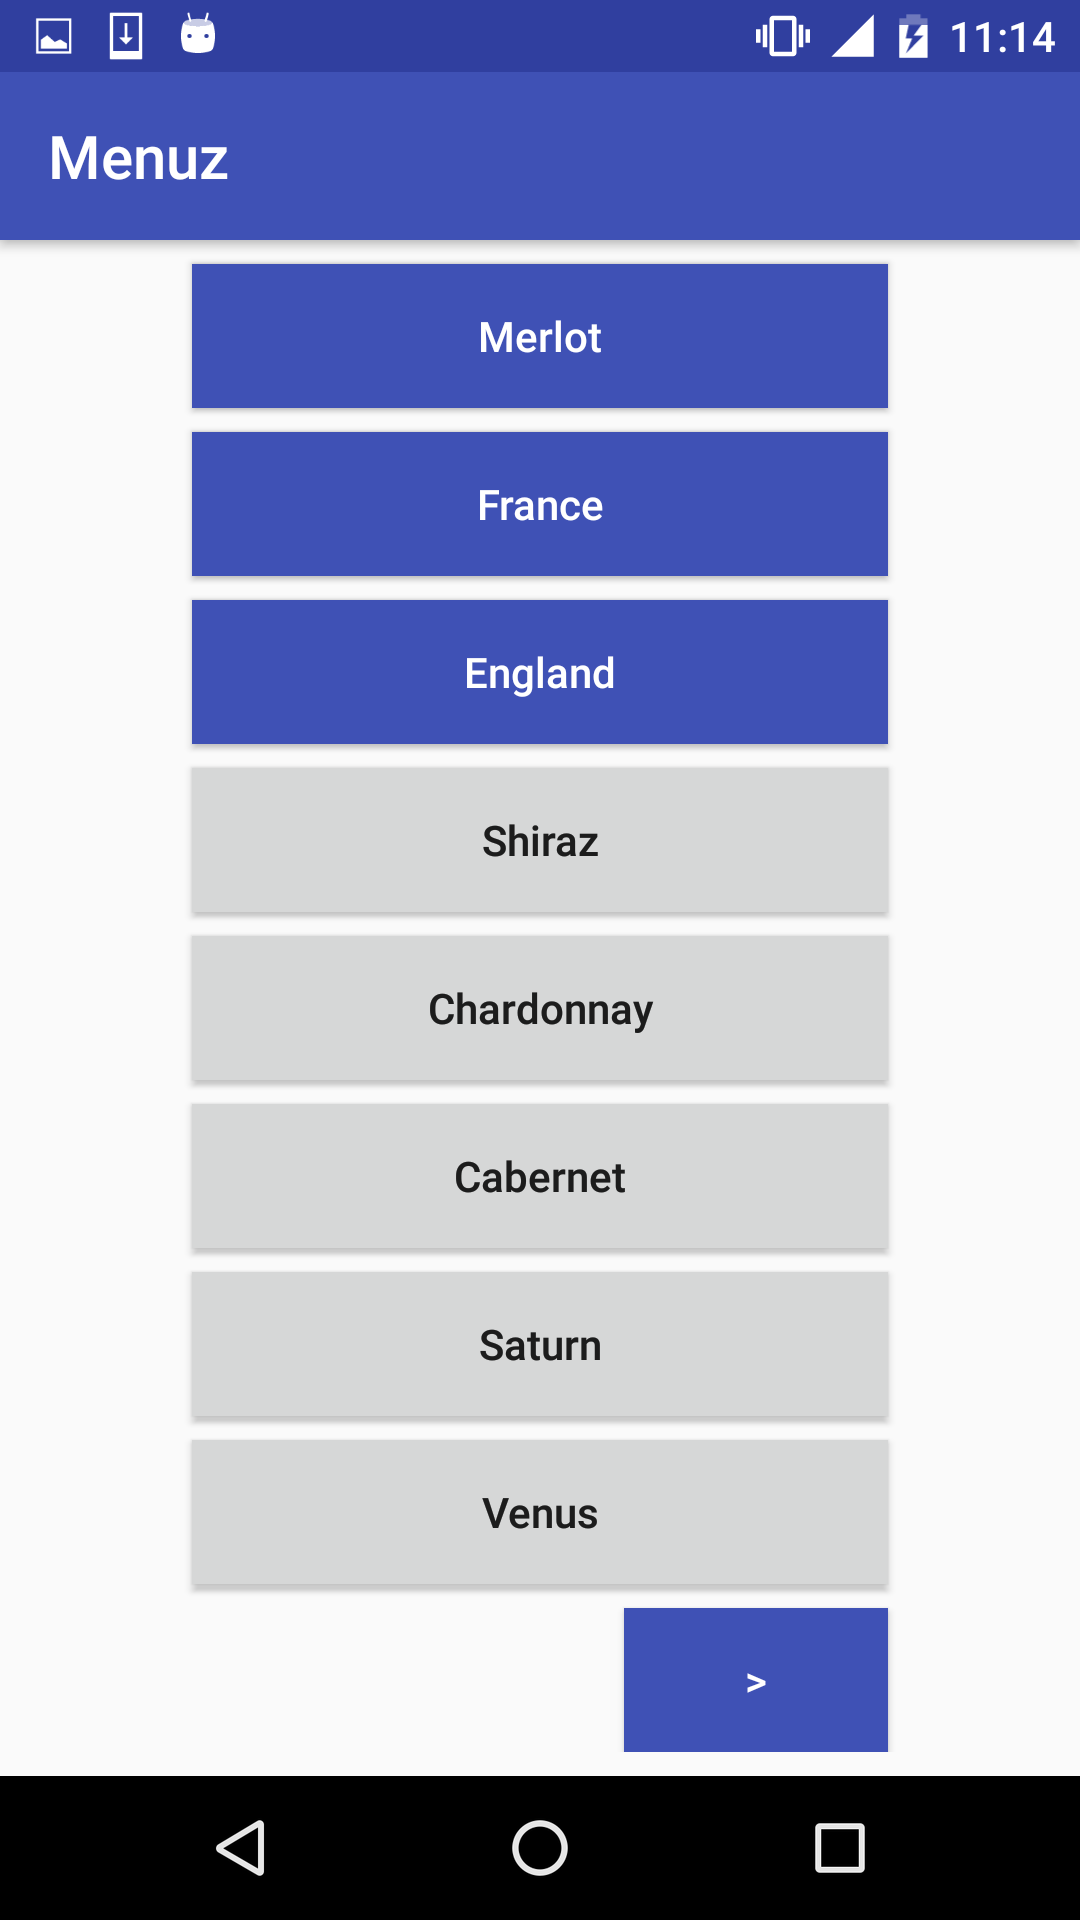
\includegraphics[scale=0.22]{img/minisplit_menu.png}
    \label{fig:minisplit_menu}
    \caption{MinimisedSplitMenuActivity.}
  \end{center}
\end{figure}

\newpage

\begin{figure}[!ht]
  \begin{center}
    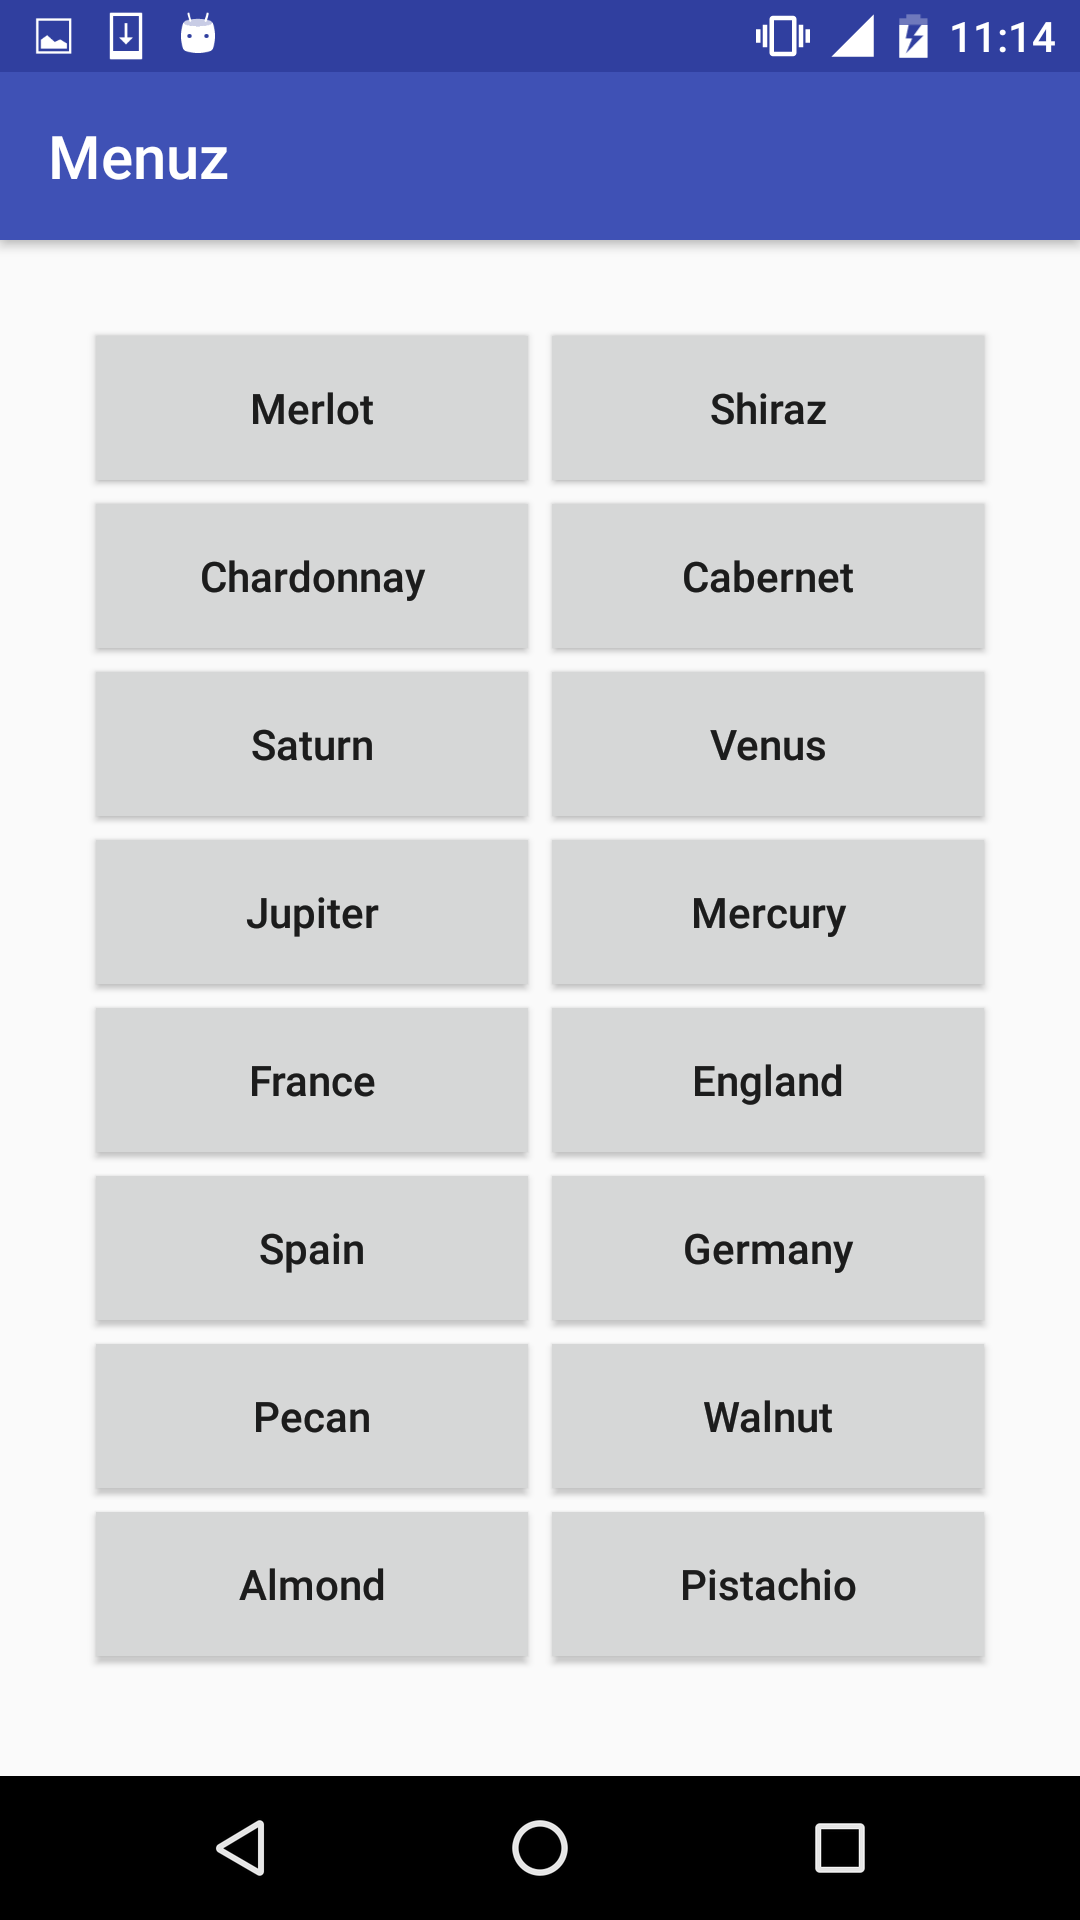
\includegraphics[scale=0.22]{img/resp_menu.png}
    \label{fig:resp_menu}
    \caption{ResponsiveMenuActivity.}
  \end{center}
\end{figure}

\newpage

\begin{figure}[!ht]
  \begin{center}
    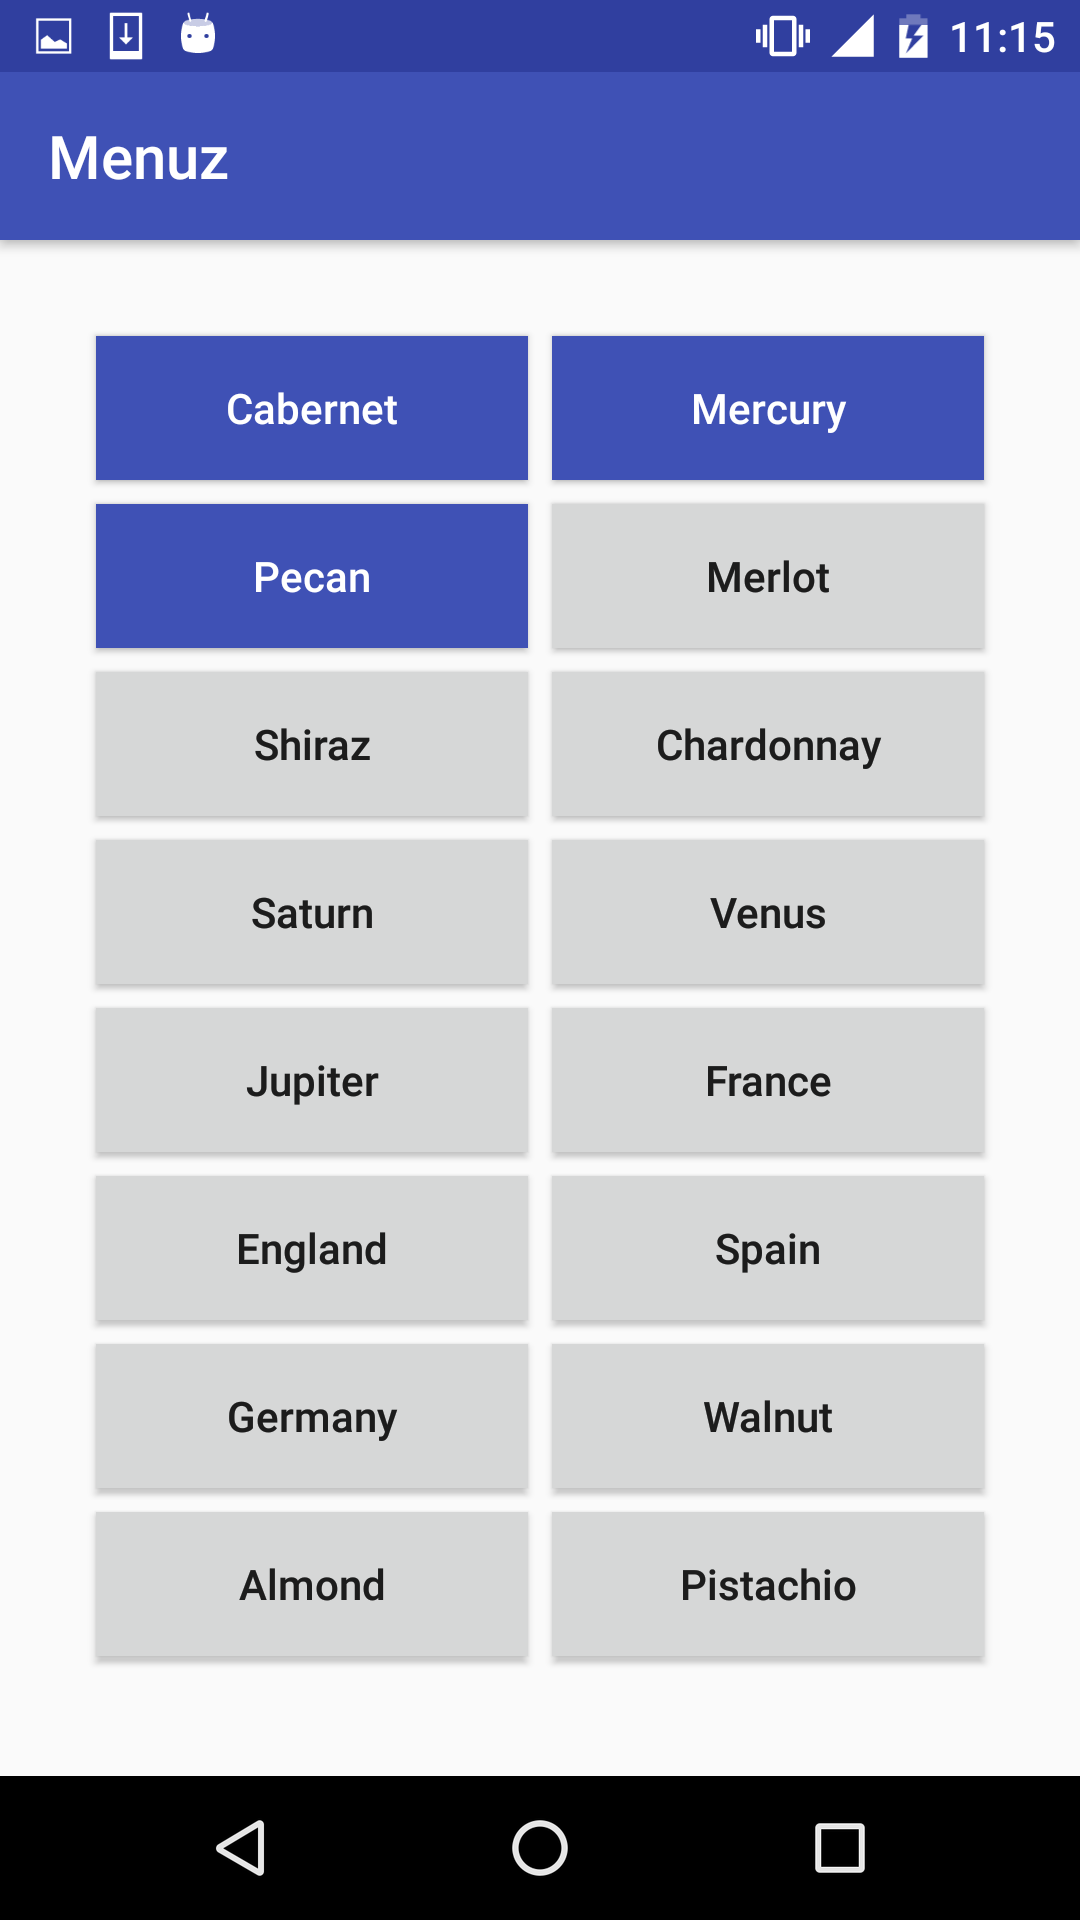
\includegraphics[scale=0.22]{img/respsplit_menu.png}
    \label{fig:respsplit_menu}
    \caption{ResponsiveSplitMenuActivity.}
  \end{center}
\end{figure}

\newpage

\begin{figure}[!ht]
  \begin{center}
    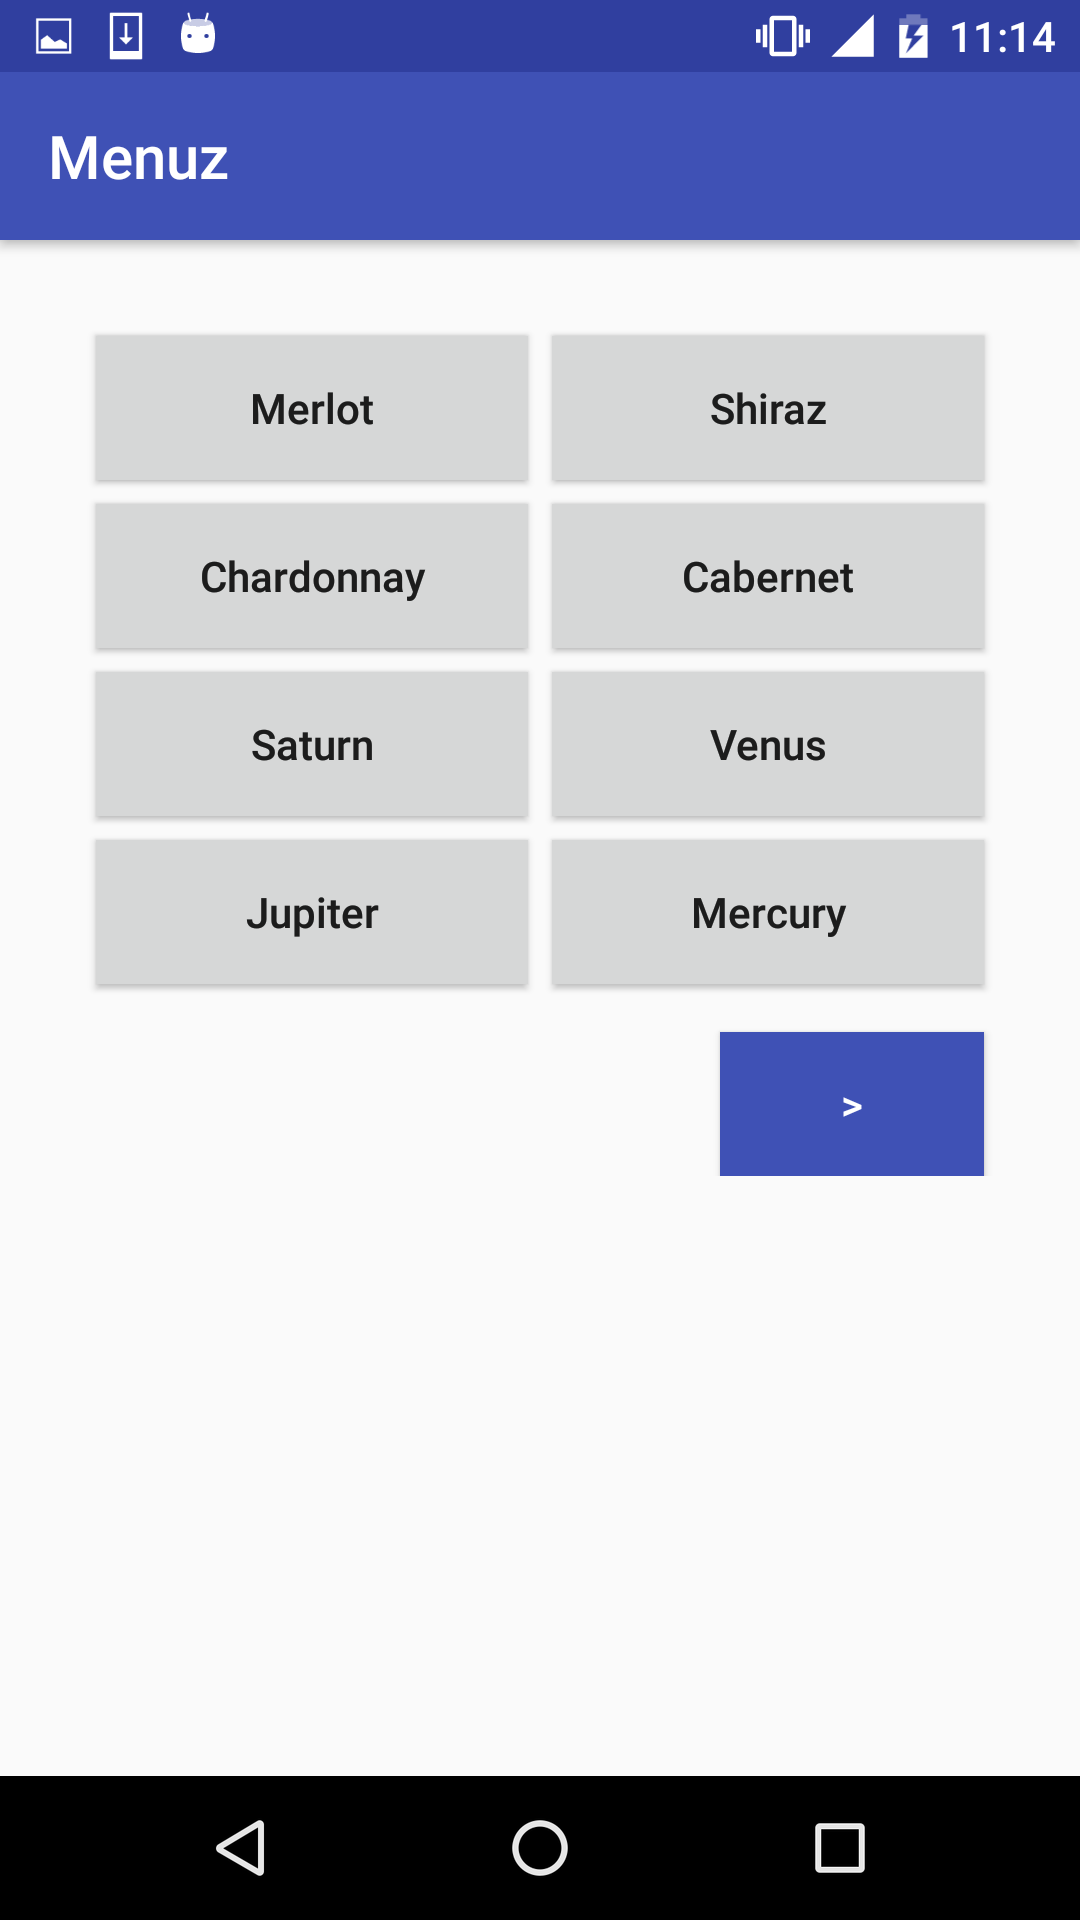
\includegraphics[scale=0.22]{img/miniresp_menu.png}
    \label{fig:miniresp_menu}
    \caption{MinimisedResponsiveMenuActivity.}
  \end{center}
\end{figure}

\newpage

\begin{figure}[!ht]
  \begin{center}
    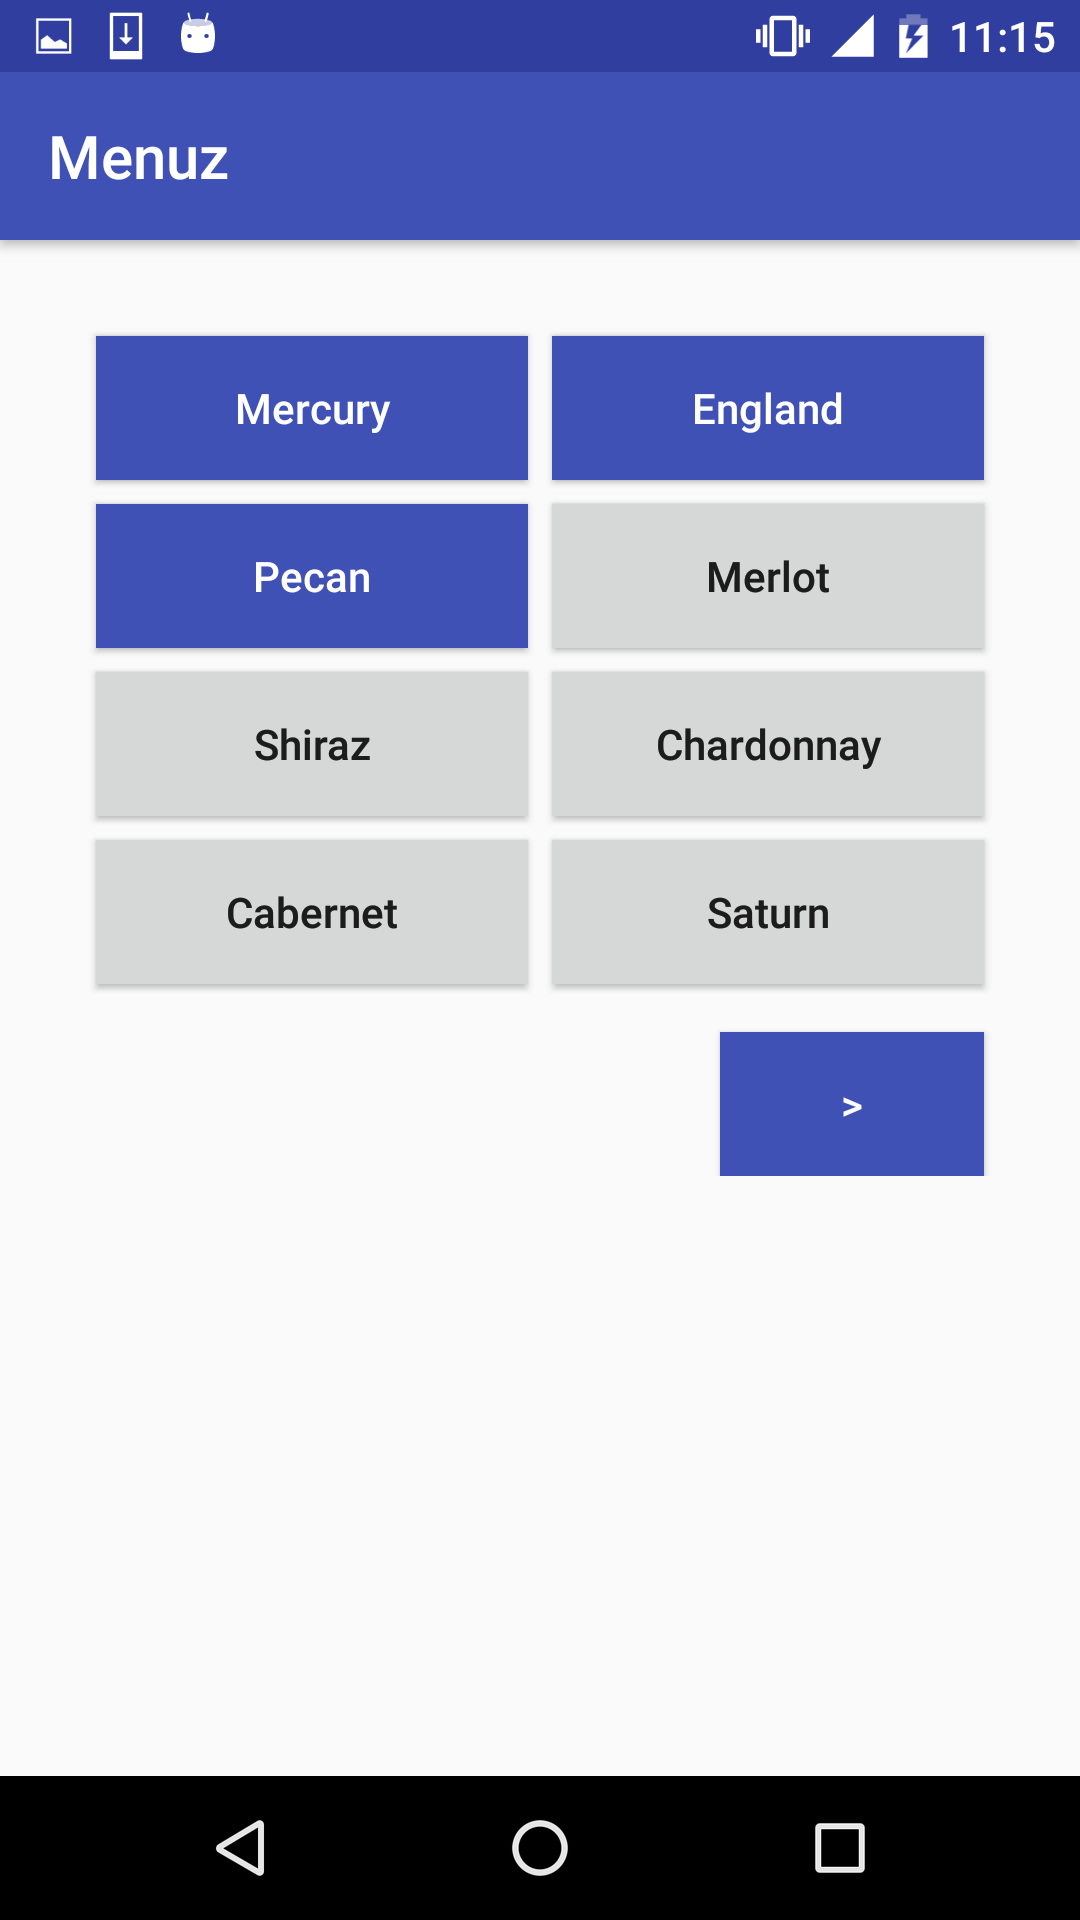
\includegraphics[scale=0.22]{img/minirespsplit_menu.png}
    \label{fig:minirespsplit_menu}
    \caption{MinimisedResponsiveSplitMenuActivity.}
  \end{center}
\end{figure}

\newpage

\begin{figure}[!ht]
  \begin{center}
    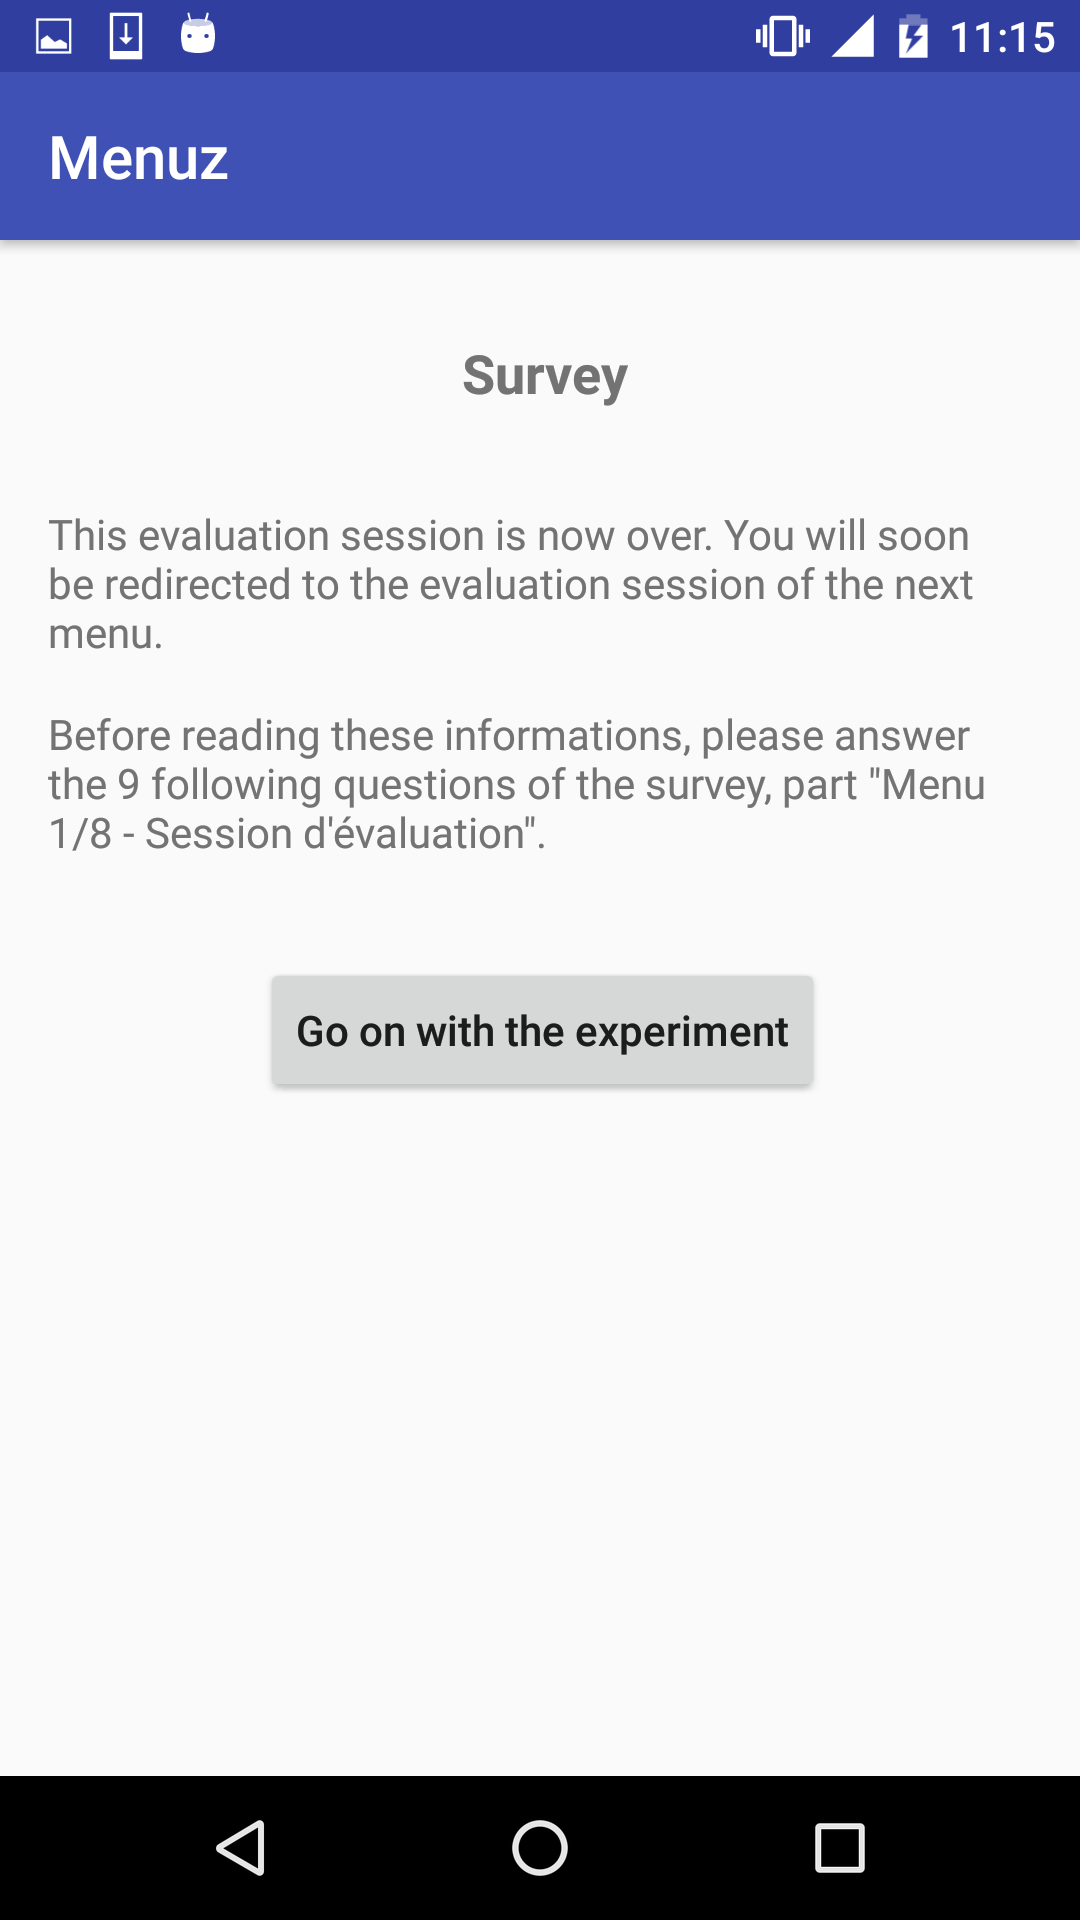
\includegraphics[scale=0.22]{img/survey_activity.png}
    \label{fig:survey_activity}
    \caption{SurveyActivity, at the end of the 1st evaluation session.}
  \end{center}
\end{figure}

\newpage

\begin{figure}[!ht]
  \begin{center}
    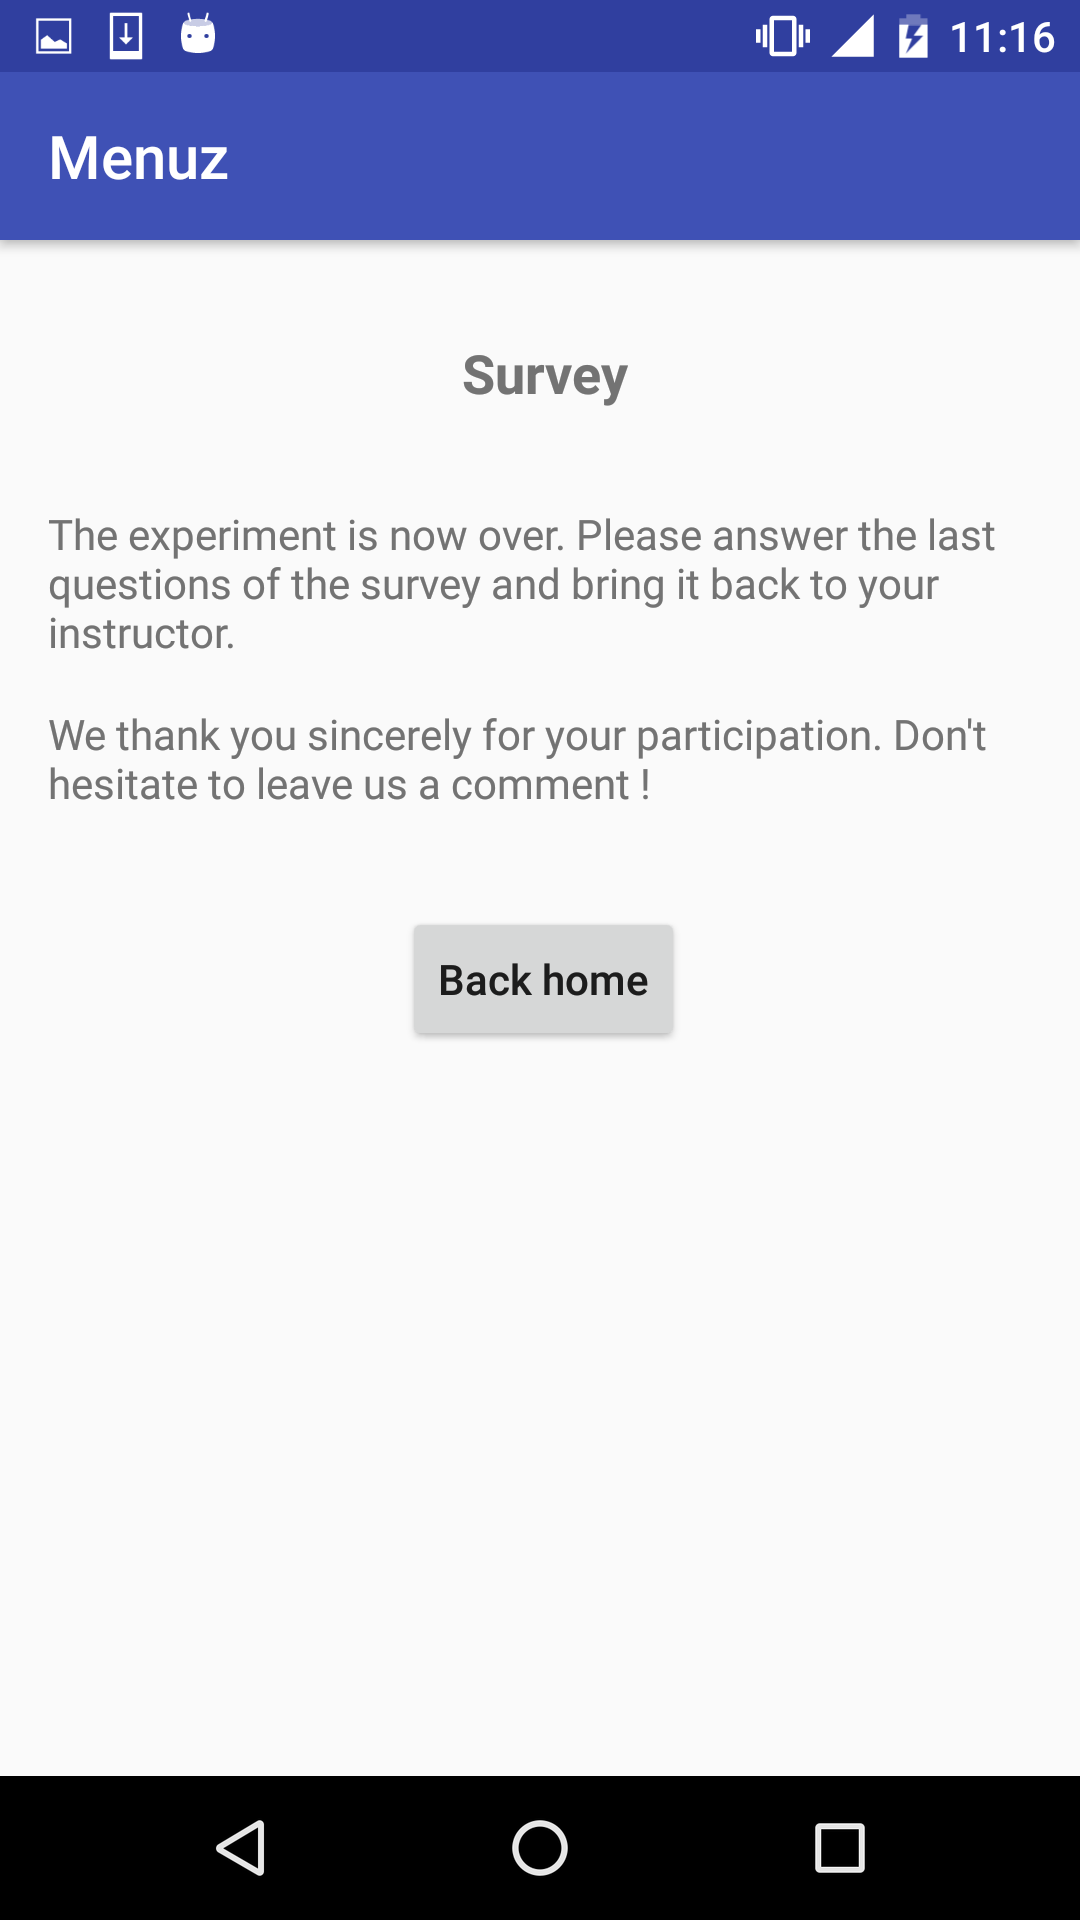
\includegraphics[scale=0.22]{img/survey_activityb.png}
    \label{fig:survey_activityb}
    \caption{SurveyActivity, at the end of the experiment.}
  \end{center}
\end{figure}

\newpage

\chapter{Get the app (How to)}
The Android application developed during the experiment is available as an open 
source repository on GitHub, see github.com/nmagrofuoco/menuz. The 
application is currently implemented in its French version. A readme file is 
available to switch the application to its English version. The repository also 
stores the sources of the dissertation.


\includepdf[pages={3-4}]{cover/cover.pdf}





\end{document}